% diss_lzh main file
%********************************************************
\documentclass[a4paper,BCOR5mm,11pt,headsepline,bibtotoc]{scrbook}



\usepackage[margin={0.2cm,0.2cm}]{caption}
\usepackage[super]{nth}

\usepackage{times,amsmath,epsfig}
\usepackage{amssymb}
\usepackage{amsmath}
\usepackage{amsfonts}
\usepackage[ruled,linesnumbered]{algorithm2e}
\usepackage{graphicx}
%\usepackage{subfig}
\usepackage{caption}
\usepackage{array}
\usepackage{booktabs}
\usepackage{epstopdf}
\usepackage{subcaption}

\usepackage{comment}

\usepackage{listings}
\usepackage{xcolor}

\usepackage{color,soul}
\usepackage{multirow}
%\usepackage[options]{natbib}

\usepackage{CJKutf8}
\usepackage[utf8]{inputenc}
\usepackage{amsthm}
\usepackage{thmtools,thm-restate}
\usepackage{bbm}

\usepackage[hyphens]{url}
\def\UrlBreaks{\do\/\do-}

\colorlet{punct}{red!60!black}
\definecolor{background}{HTML}{EEEEEE}
\definecolor{delim}{RGB}{20,105,176}
\colorlet{numb}{magenta!60!black}

\DeclareMathOperator*{\argmax}{arg\,max} 

\newcommand{\TODO}[1]{{TODO:#1}}
\newcommand{\rima}[1]{\textbf{(Rima: #1)}}

\usepackage{todonotes}

%%\newtheorem{definition}{Definition}
\theoremstyle{definition}
\newtheorem{definition}{Definition}[section]
\newtheorem{theorem}{Theorem}
\newtheorem{lemma}{Lemma}
\newtheorem{proposition}[theorem]{Proposition}
\newtheorem{corollary}[theorem]{Corollary}

\newtheorem{example}{Example}

\usepackage[utf8]{inputenc}
\usepackage[english]{babel}


%\renewcommand{\baselinestretch}{2.0}


\def\proofsketch{\noindent\hspace{1em}{\itshape Proof Outline: }}
%\def\endproofsketch{\hspace*{\fill}~\qed\par\endtrivlist\unskip}

% correct bad hyphenation here
\hyphenation{op-tical net-works semi-conduc-tor}
\newcommand{\hlc}[1]{{\sethlcolor{gray}\hl{#1}}}

%\newtheorem{research}{Research Question}%[chapter]
\declaretheorem[name=Research Question]{research}
\declaretheorem[name=Future Work]{future}
%\newtheorem{hypothesis}{Hypothesis}[chapter]
\declaretheorem[parent=research]{hypothesis}
\newtheorem{contribution}{Contribution}
\declaretheorem[numbered=no]{principal}

\setlength{\parindent}{0pt}
\newcommand{\forceindent}{\leavevmode{\parindent=1em\indent}}
\newcommand{\SubItem}[1]{
    {\setlength\itemindent{15pt} \item[-] #1}
}

\usepackage{listings}
\usepackage{xcolor}

\colorlet{punct}{red!60!black}
\definecolor{background}{HTML}{EEEEEE}
\definecolor{delim}{RGB}{20,105,176}
\colorlet{numb}{magenta!60!black}

\lstdefinelanguage{json}{
    basicstyle=\scriptsize\ttfamily,
    numbers=left,
    numberstyle=\scriptsize,
    stepnumber=0,
    numbersep=8pt,
    showstringspaces=false,
    breaklines=true,
    frame=lines,
    backgroundcolor=\color{background},
    literate=
%     *{0}{{{\color{numb}0}}}{1}
%      {1}{{{\color{numb}1}}}{1}
%      {2}{{{\color{numb}2}}}{1}
%      {3}{{{\color{numb}3}}}{1}
%      {4}{{{\color{numb}4}}}{1}
%      {5}{{{\color{numb}5}}}{1}
%      {6}{{{\color{numb}6}}}{1}
%      {7}{{{\color{numb}7}}}{1}
%      {8}{{{\color{numb}8}}}{1}
%      {9}{{{\color{numb}9}}}{1}
%      {:}{{{\color{punct}{:}}}}{1}
%      {,}{{{\color{punct}{,}}}}{1}
%      {\{}{{{\color{delim}{\{}}}}{1}
%      {\}}{{{\color{delim}{\}}}}}{1}
%      {[}{{{\color{delim}{[}}}}{1}
%      {]}{{{\color{delim}{]}}}}{1},
}

\usepackage{hyperref}
\hypersetup{
    colorlinks,
    citecolor=black,
    filecolor=black,
    linkcolor=black,
    urlcolor=black
}

\usepackage{currvita}
\usepackage{outlines}


\usepackage[ngerman, english]{babel} % Englische und Deutsche Version
% Standard-Dokument mit
%   Papierformat A4
%   Binderand 5 mm
%   Schrift 12-Punkt
%   Linie unter der Kopfzeile
%   Nummern ohne Punkt am Ende
%   Literaturverzeichnis mit Nummer im Inhaltsverzeichnis
%\usepackage{setspace}
%\onehalfspacing
%********************************************************
% Parameters and Counters
\newcounter{def_counter}
%\refstepcounter{def_counter}
% Größe anpassen
%\usepackage{setspace}
%\usepackage{geometry}

\usepackage{graphicx}
%\usepackage{epsfig}
%\usepackage[german]{varioref}

%\usepackage{longtable}
%\usepackage{ltxtable}
\usepackage{boxedminipage}

% Index-Packet
\usepackage{makeidx}

% Wrap-Figures
\usepackage{wrapfig}

% \usepackage{palatino}

% Fonts etc:
% 8-Bit-Fonts
\usepackage[T1]{fontenc}
% Web-Addressen auch mit T1-Encoding
\usepackage[T1]{url}
% und in sf-Font
\urlstyle{sf}

%   zusaetzliche Symbole
\usepackage{textcomp,latexsym,amsfonts}

%   Mac-Umlaute in der Eingabe
%\usepackage[latin1]{inputenc}

% Schlüssel für Literaturverweise anzeigen
% \usepackage{showkeys}

\setlength{\emergencystretch}{20pt} \tolerance=4000

% für Algorithmen
%\usepackage{algorithmic}
%\usepackage[Algorithmus]{algorithm}

% neue deutsche Rechtschreibung
%\usepackage{ngerman}

% korrekte Spaces nach Makros
\usepackage{xspace}

% fuer die aktuelle Zeit
\usepackage{scrtime}

% Literaturverweise mit (Autor Jahr) nach DIN
%\usepackage{natbib}

% Literaturverweise mit pnnamed
\usepackage{pnnamed}


% Für Programm Listings
\usepackage{listings}
% example
%\lstset{language=Java} ...
%\begin{lstlisting}{}
%for(int i=0; i<n; i++)
%    cout << "loop";
%\end{lstlisting}


\makeatletter

% Eigenes Verzeichnis für fixme-Vermerke
\def\listoffixmes{
  \chapter*{Liste von FIXME-Vermerken}
    \@starttoc{fxm}
    }
%\def\listoffixmes{}

% fixme-Vermerk
%%%%\newcommand{\fixme}[1]{\marginpar{\raggedright\small{\bf FIXME:} {\em#1}}}
\newcommand{\fixme}[1]{ %
  \addcontentsline{fxm}{figure}{\thesubsection{} #1} %
  \marginpar{%
    \begin{boxedminipage}{\marginparwidth}%
      {\small%
        {\bf FIXME:}\\%
        {\em  #1}%
        }%
    \end{boxedminipage}%
    }\xspace%
  }

%\newcommand{\fixme}[1]{}

\newcommand{\largefixme}[1]{
  \addcontentsline{fxm}{figure}{\thesubsection{} #1}
  \begin{boxedminipage}{\textwidth}
    {\bf FIXME:}\\
    {\em  #1}
  \end{boxedminipage}
  }

% Anmerkungen von Lektoren
\newcommand{\ysu}[1]{
 \normalfont{\textbf{YSu:} \em #1\/}
}
\newcommand{\sha}[1]{
 \normalfont{\textbf{SHa:} \em #1\/}
}
\newcommand{\rst}[1]{
 \normalfont{\textbf{RSt:} \em #1\/}
}
\newcommand{\sst}[1]{
 \normalfont{\textbf{SSt:} \em #1\/}
}
\newcommand{\gst}[1]{
 \normalfont{\textbf{GSt:} \em #1\/}
}

% Guide Umgebung für die Übersichten am Anfang von
% Kapiteln und Abschnitten
\newcommand{\contendguide}[1]{
\begin{tabular}{lr}
\parbox{2cm}{\includegraphics[width=2cm]{./figs/contendguide.eps}}
& \parbox{10cm}{\setlength{\parskip}{1ex plus0.5ex minus0.2ex} #1}\\
\end{tabular}
}

% Abkürzungen
\newcommand{\methodology}{On-To-Knowledge Methodology}
\newcommand{\kmp}{Knowledge Meta Process}
\newcommand{\kp}{Knowledge Process}

% Description ändern
\renewcommand*\descriptionlabel[1]{\hspace\labelsep
                                \normalfont{\em #1\/} \hskip 1em plus 1em}

% Bezeichner etc. im Text
\newcommand{\code}{\sf}

% Auslassung [...] bei Zitaten
\newcommand{\ausl}{$[\ldots]$\xspace}

% Absatzabstand etwas groesser
\setlength{\parskip}{1ex plus0.5ex minus0.2ex}

% Abstand zweier Listenelemente kleiner
\setlength{\itemsep}{0ex plus0.2ex}

% Keine Absatz-Einrückung
\setlength{\parindent}{0cm}

% description-Umgebung ändern
% \renewcommand{\descriptionlabel}[1]{\hspace{\labelsep}{\em #1}}

% tag for the beginning of a new file
\newcommand{\filetag}[1]{\marginpar{\tiny\bf #1}}

% Drei Ebenen numerieren
\setcounter{secnumdepth}{2} \setcounter{tocdepth}{2}

% Helps LaTeX put figures where YOU want
\renewcommand{\topfraction}{0.9}    % 90% of page top can be a float
\renewcommand{\bottomfraction}{0.9} % 90% of page bottom can be a float
\renewcommand{\textfraction}{0.1}   % only 10% of page must to be text

\makeatother

% Extra-Abstand nach Satzende
\nonfrenchspacing

% Helvetica-Schrift für den Entwurf, später wieder Roman
% \renewcommand{\familydefault}{phv}

% Konzepte, Relationen etc. ...
\def\rel#1{\mbox{\small\textsc{#1}}}
\def\conc#1{\mbox{\textsf{#1}}}
\def\inst#1{\mbox{\small{\texttt{#1}}}}
\def\axiom#1{\mbox{\textit{#1}}}
\def\var#1{\mbox{\textsl{#1}}}
\def\code#1{\mbox{\small{\texttt{#1}}}}
\def\lex#1{\mbox{{\small``\textsf{#1}''}}}
\def\impliedBy{\leftarrow}
\def\slot{\rightarrow\hspace{-1.3ex}\rightarrow}
\def\tslot{\Rightarrow\hspace{-1.3ex}\Rightarrow}
\def\parabold#1{\vspace{2pt}\noindent\textbf{#1}}

% KA Perspective Defs.
\usepackage{concepts}

\newcommand{\cC}{C}
\newcommand{\cL}{\mathcal{L}}
\newcommand{\cR}{R}
\newcommand{\cO}{\mathcal{O}}
\newcommand{\cA}{A}
\newcommand{\cU}{U}
\newcommand{\cS}{S}
\newcommand{\cSC}{\cS_\cC}
\newcommand{\cSR}{\cS_\cR}
\newcommand{\Ref}{\mathit{Ref}}
\newcommand{\RefC}{\Ref_C}
\newcommand{\RefR}{\Ref_R}

\newcommand{\dom}{\mathrm{dom}}
\newcommand{\range}{\mathrm{range}}
\newcommand{\KB}{\mathit{KB}}
\newcommand{\IL}{\mathit{IL}}
%\newcommand{\IR}{\mathit{IR}}
\newcommand{\Lex}{\mathit{Lex}}

%\newcommand{\powerset}{\mathfrak{P}}
\newcommand{\seml}{[\![}
\newcommand{\semr}{]\!]}
\newcommand{\sem}[1]{\seml #1 \semr}


% TM (Trademark)
\def\tm#1{#1\raisebox{1ex}{\fontsize{6}{1}\selectfont\texttt{TM}}}

% Mathe Krams aus dem Web

%\newtheorem{theorem}{Theorem}[section]
%\newtheorem{lemma}[theorem]{Lemma}
%\newtheorem{proposition}[theorem]{Proposition}
%\newtheorem{corollary}[theorem]{Corollary}
%
%\newenvironment{proof}[1][Proof]{\begin{trivlist}
%\item[\hskip \labelsep {\bfseries #1}]}{\end{trivlist}}
%\newenvironment{definition}[1][Definition]{\begin{trivlist}
%\item[\hskip \labelsep {\bfseries #1}]}{\end{trivlist}}
%\newenvironment{example}[1][Example]{\begin{trivlist}
%\item[\hskip \labelsep {\bfseries #1}]}{\end{trivlist}}
%\newenvironment{remark}[1][Remark]{\begin{trivlist}
%\item[\hskip \labelsep {\bfseries #1}]}{\end{trivlist}}
%
%\newcommand{\qed}{\nobreak \ifvmode \relax \else
%      \ifdim\lastskip<1.5em \hskip-\lastskip
%      \hskip1.5em plus0em minus0.5em \fi \nobreak
%      \vrule height0.75em width0.5em depth0.25em\fi}

%********************************************************
% Create the index
\makeindex
%********************************************************
\begin{document}


% Tabellen etwas gr��er
\renewcommand{\arraystretch}{1.25}
\setlength{\parindent}{3em}
\setlength{\parskip}{0.3em}
%********************************************************
% \nocite*
%Nummern anders
%********************************************************
\frontmatter


\titlehead{}

\title{Short Text Categorization by Leveraging Knowledge Bases}
%Leveraging Knowledge Graphs for Text Categorization

\subtitle{%\disssubtitle
	%{\Large Using Standards}
	\vskip 15mm
	\begin{otherlanguage}{ngerman}
		{\normalsize \textmd{
				Zur Erlangung des akademischen Grades eines\\ 
				Doktors der Ingenieurwissenschaften\\
				(Dr.-Ing.)\\
				\vskip 5mm
				bei der Fakult\"at f\"ur Wirtschaftswissenschaften\\ 
				des Karlsruher Instituts f\"ur Technologie (KIT)\\
				\vskip 15mm
				%eingereichte\\
				genehmigte\\
				DISSERTATION\\
			}}
		\end{otherlanguage}
		\vskip 0mm
	}

\author{
	{\normalsize \sffamily von}\\
	Dipl.-Inform. Rima Türker
}
\date{}

\publishers{
  \begin{normalsize}
  \begin{flushleft}
   \begin{tabular}{p{1.2cm}rl}
    & \textbf{Tag der m\"{u}ndlichen Pr\"{u}fung:} & -\\
    & \textbf{Referent:} & Prof. Dr. Harald Sack\\
    & \textbf{Korreferent:} & Prof. Dr. - \\
%    & \textbf{Pr\"{u}fer:} & Prof. Dr. York Sure-Vetter \\
%    & \textbf{Vorsitzende:} & Prof. Dr. Melanie Schienle \\
    \end{tabular}
 \end{flushleft}
%    \textbf{Vorsitzender der Pr\"{u}fungskommission:} \\

    \end{normalsize}
}


%\lowertitleback{\small This document was created on \today{}}

\dedication{To -.}

\maketitle

\maketitle
%********************************************************
% Preface and Acknowledgements
\chapter{Abstract}


%%\chapter{Publications}
\chapter{Foreword}

The contributions presented in this thesis have been published at various workshops, conferences and journals. Firstly, I list the most important publications that directly contribute to this thesis with regard to \emph{semantic annotation}, \emph{semantic search} and \emph{cross-lingual semantics}, as follows:

\forceindent\textbf{Semantic Annotation}
\begin{itemize}
    \item Lei Zhang, Achim Rettinger, Patrick Philipp: Context-Aware Entity Disambiguation in Text Using Markov Chains. In \emph{Proceedings of the 2016 IEEE/WIC/ACM International Conferences on Web Intelligence (WI 2016), Omaha, Nebraska, USA, October 13-16, 2016.}~\cite{wi2016}
%    \textbf{(Long Paper)}
    \item Lei Zhang, Cong Liu, Achim Rettinger: A Topic-Sensitive Model for Salient Entity Linking. In \emph{Proceedings of the 3rd International Workshop on Linked Data for Information Extraction (LD4IE) co-located with the 14th International Semantic Web Conference (ISWC 2015), Bethlehem, Pennsylvania, USA, October 11-15, 2015.}~\cite{DBLP:conf/semweb/ZhangLR15}
%    \textbf{(Long Paper)}
\end{itemize}

\forceindent\textbf{Semantic Search}
\begin{itemize}
    \item Lei Zhang, Achim Rettinger, Ji Zhang: A Probabilistic Model for Time-Aware Entity Recommendation. In \emph{Proceedings of the 15th International Semantic Web Conference (ISWC 2016), Kobe, Japan, October 17-21, 2016.}~\cite{DBLP:conf/semweb/ZhangRZ16a}
%    \textbf{(Long Paper)}
    \textbf{Best Student Research Paper}
    \item Lei Zhang, Thanh Tran, Achim Rettinger: Probabilistic Query Rewriting for Efficient and Effective Keyword Search on Graph Data. In \emph{Proceedings of the VLDB Endowment of the 39th International Conference on Very Large Data Bases (VLDB 2013) Volume 6, Number 14, September 2013.}~\cite{DBLP:journals/pvldb/0007TR13}
%    \textbf{(Long Paper)}
\end{itemize}

\forceindent\textbf{Cross-lingual Semantics}
\begin{itemize}
    \item  Lei Zhang, Achim Rettinger, Ji Zhang: A Knowledge Base Approach to Cross-lingual Keyword Query Interpretation. In \emph{Proceedings of the 15th International Semantic Web Conference (ISWC 2016), Kobe, Japan, October 17-21, 2016.}~\cite{DBLP:conf/semweb/ZhangRZ16}
%    \textbf{(Long Paper)}
    \item Lei Zhang, Michael Färber, Achim Rettinger: XKnowSearch! Exploiting Knowledge Bases for Entity-based Cross-lingual Information Retrieval. In \emph{Proceedings of the 25th ACM International Conference on Information and Knowledge Management (CIKM 2016), Indianapolis, USA, October 24-28, 2016.}~\cite{DBLP:conf/cikm/Zhang16}
%    \textbf{(Demo Paper)}
    \item Lei Zhang, Achim Rettinger: X-LiSA: Cross-lingual Semantic Annotation. In \emph{ Proceedings of the VLDB Endowment of the 40th International Conference on Very Large Data Bases (VLDB 2014), Volume 7, Number 13, August 2014.}~\cite{xlisa}
%    \textbf{(Demo Paper)}
    \item Lei Zhang, Michael Färber, Achim Rettinger: xLiD-Lexica: Cross-lingual Linked Data Lexica. In \emph{Proceedings of the 9th International Conference on Language Resources and Evaluation (LREC 2014), Reykjavik, Iceland, May 26-31, 2014.}~\cite{Zhang2014}
%    \textbf{(Short Paper)}
    \item Lei Zhang, Achim Rettinger, Steffen Thoma: Bridging the Gap between Cross-lingual NLP and DBpedia by Exploiting Wikipedia. In \emph{Proceedings of the NLP{\&}DBpedia workshop co-located with the 13th International Semantic Web Conference (ISWC 2014), Riva del Garda, Italy, October 19-23, 2014.}~\cite{zhang2014btgbcnadbew}
\end{itemize}

In the course of writing this thesis, I have published several other papers, which helped me to shape the focus of the present work. They could be considered as related work:  

\forceindent\textbf{Other Publications}
\begin{itemize}
    \item Lei Zhang, Michael Färber, Andreas Thalhammer, Aditya Mogadala, Achim Rettinger: Exploiting Knowledge Bases for Multilingual and Cross-lingual Semantic Annotation and Search. \emph{The Semantic Web Challenge co-located with the 14th International Semantic Web Conference (SWC 2015), Bethlehem, Pennsylvania, USA, October 11-15, 2015.}~\cite{zhang2015swc} 
    \textbf{2nd Prize Winner}
    \item Lei Zhang, Thanh Tran, Achim Rettinger: A Theoretical Analysis of Cross-lingual Semantic Relatedness in Vector Space Models. In \emph{Proceedings of the 2015 International Conference on The Theory of Information Retrieval (ICTIR 2015), Northampton, Massachusetts, USA, September 27-30, 2015.}~\cite{DBLP:conf/ictir/0007TR15}
%    \textbf{(Long Paper)}
    \item Lei Zhang, Yunpeng Dong, Achim Rettinger: Towards Entity Correctness, Completeness and Emergence for Entity Recognition. In \emph{Proceedings of the 24th International Conference on World Wide Web Companion (WWW 2015), Florence, Italy, May 18-22, 2015.}~\cite{DBLP:conf/www/ZhangDR15}
%%    \textbf{(Short Paper)}
    \item Lei Zhang, Wentao Chen, Thanh Tran, Achim Rettinger: Time-Aware Entity Search in DBpedia. \emph{The Semantic Web: ESWC 2015 Satellite Events, Portorož, Slovenia, May 31 - June 4, 2015.}~\cite{DBLP:conf/esws/0034CTR15}
%    \textbf{(Short Paper)}
    \item Thanh Tran, Lei Zhang: Keyword Query Routing. \emph{IEEE Transactions on Knowledge and Data Engineering (TKDE), Volume 26, Number 2, February 2014.}~\cite{DBLP:journals/tkde/Tran014}
%    \textbf{(Long Paper)}
    \item Lei Zhang, Achim Rettinger: Semantic Annotation, Analysis and Comparison: A Multilingual and Cross-lingual Text Analytics Toolkit. In \emph{Proceedings of the 14th Conference of the European Chapter of the Association for Computational Linguistics (EACL 2014), Gothenburg, Sweden, April 26-30, 2014.}~\cite{DBLP:conf/eacl/ZhangR14}
%    \textbf{(Demo Paper)}
    \item Xavier Carreras, Lluís Padró, Lei Zhang, Achim Rettinger, Zhixing Li, Esteban García-Cuesta, Zeljko Agic, Bozo Bekavac, Blaz Fortuna, Tadej Stajner: XLike Project Language Analysis Services. In \emph{Proceedings of the 14th Conference of the European Chapter of the Association for Computational Linguistics (EACL 2014), Gothenburg, Sweden, April 26-30, 2014.}~\cite{DBLP:conf/eacl/CarrerasP0RLGABFS14}
%    \textbf{(Demo Paper)}
    \item Michael Färber, Lei Zhang, Achim Rettinger: Kuphi - an Investigation Tool for Searching for and via Semantic Relations. \emph{The Semantic Web: ESWC 2014 Satellite Events, Anissaras, Crete, Greece, May 25-29, 2014.}~\cite{DBLP:conf/esws/Farber0R14}
%    \textbf{(Demo Paper)}
    \item 	Achim Rettinger, Lei Zhang, Dasa Berovic, Danijela Merkler, Matea Srebacic, Marko Tadic: RECSA: Resource for Evaluating Cross-lingual Semantic Annotation. In \emph{Proceedings of the 9th International Conference on Language Resources and Evaluation (LREC 2014), Reykjavik, Iceland, May 26-31, 2014.}~\cite{DBLP:conf/lrec/RettingerZBMST14}
%    \textbf{(Short Paper)}
    \item Lei Zhang, Michael Färber, Thanh Tran, Achim Rettinger: Exploiting Semantic Annotations for Entity-based Information Retrieval. In \emph{Proceedings of the ISWC 2014 Posters \& Demonstrations Track a track within the 13th International Semantic Web Conference (ISWC 2014), Riva del Garda, Italy, October 19-23, 2014.}~\cite{DBLP:conf/semweb/0007FTR14}
%    \textbf{(Short Paper)}
    \item Lei Zhang, Achim Rettinger, Michael Färber, Marko Tadic: A Comparative Evaluation of Cross-Lingual Text Annotation Techniques. \emph{Information Access Evaluation. Multilinguality, Multimodality, and Visualization - 4th International Conference of the CLEF Initiative (CLEF 2013), Valencia, Spain, September 23-26, 2013.}~\cite{DBLP:conf/clef/ZhangRFT13}
%    \textbf{(Long Paper)}
    \item Thanh Tran, Lei Zhang, Rudi Studer: Summary Models for Routing Keywords to Linked Data Sources. In \emph{Proceedings of the 9th International Semantic Web Conference (ISWC 2010), Shanghai, China, November 7-11, 2010.}~\cite{DBLP:conf/semweb/TranZS10}
%    \textbf{(Long Paper)}
\end{itemize}


%\begin{itemize}
%    \item  Lei Zhang, Achim Rettinger, Ji Zhang: A Knowledge Base Approach to Cross-lingual Keyword Query Interpretation. In \emph{Proceedings of the 15th International Semantic Web Conference (ISWC 2016), Kobe, Japan, October 17-21, 2016.}~\cite{DBLP:conf/semweb/ZhangRZ16}
%%    \textbf{(Long Paper)}
%    
%    \item Lei Zhang, Achim Rettinger, Ji Zhang: A Probabilistic Model for Time-Aware Entity Recommendation. In \emph{Proceedings of the 15th International Semantic Web Conference (ISWC 2016), Kobe, Japan, October 17-21, 2016.}~\cite{DBLP:conf/semweb/ZhangRZ16a}
%%    \textbf{(Long Paper)}
%    \textbf{Best Student Research Paper}
%    
%    \item Lei Zhang, Achim Rettinger, Patrick Philipp: Context-Aware Entity Disambiguation in Text Using Markov Chains. In \emph{Proceedings of the 2016 IEEE/WIC/ACM International Conferences on Web Intelligence (WI 2016), Omaha, Nebraska, USA, October 13-16, 2016.}~\cite{wi2016}
%%    \textbf{(Long Paper)}
%    
%    \item Lei Zhang, Michael Färber, Achim Rettinger: XKnowSearch! Exploiting Knowledge Bases for Entity-based Cross-lingual Information Retrieval. In \emph{Proceedings of the 25th ACM International Conference on Information and Knowledge Management (CIKM 2016), Indianapolis, USA, October 24-28, 2016.}~\cite{DBLP:conf/cikm/Zhang16}
%%    \textbf{(Demo Paper)}
%    
%    \item Lei Zhang, Michael Färber, Andreas Thalhammer, Aditya Mogadala, Achim Rettinger: Exploiting Knowledge Bases for Multilingual and Cross-lingual Semantic Annotation and Search. \emph{The Semantic Web Challenge co-located with the 14th International Semantic Web Conference (SWC 2015), Bethlehem, Pennsylvania, USA, October 11-15, 2015.}~\cite{zhang2015swc} 
%    \textbf{2nd Prize Winner}
%    
%    \item Lei Zhang, Thanh Tran, Achim Rettinger: A Theoretical Analysis of Cross-lingual Semantic Relatedness in Vector Space Models. In \emph{Proceedings of the 2015 International Conference on The Theory of Information Retrieval (ICTIR 2015), Northampton, Massachusetts, USA, September 27-30, 2015.}~\cite{DBLP:conf/ictir/0007TR15}
%%    \textbf{(Long Paper)}
%    
%    \item Lei Zhang, Cong Liu, Achim Rettinger: A Topic-Sensitive Model for Salient Entity Linking. In \emph{Proceedings of the 3rd International Workshop on Linked Data for Information Extraction (LD4IE) co-located with the 14th International Semantic Web Conference (ISWC 2015), Bethlehem, Pennsylvania, USA, October 11-15, 2015.}~\cite{DBLP:conf/semweb/ZhangLR15}
%%    \textbf{(Long Paper)}
%    
%    \item Lei Zhang, Yunpeng Dong, Achim Rettinger: Towards Entity Correctness, Completeness and Emergence for Entity Recognition. In \emph{Proceedings of the 24th International Conference on World Wide Web Companion (WWW 2015), Florence, Italy, May 18-22, 2015.}~\cite{DBLP:conf/www/ZhangDR15}
%%%    \textbf{(Short Paper)}
%    
%    \item Lei Zhang, Wentao Chen, Thanh Tran, Achim Rettinger: Time-Aware Entity Search in DBpedia. \emph{The Semantic Web: ESWC 2015 Satellite Events, Portorož, Slovenia, May 31 - June 4, 2015.}~\cite{DBLP:conf/esws/0034CTR15}
%%    \textbf{(Short Paper)}
%    
%    \item Lei Zhang, Achim Rettinger: X-LiSA: Cross-lingual Semantic Annotation. In \emph{ Proceedings of the VLDB Endowment of the 40th International Conference on Very Large Data Bases (VLDB 2014), Volume 7, Number 13, August 2014.}~\cite{xlisa}
%%    \textbf{(Demo Paper)}
%    
%    \item Thanh Tran, Lei Zhang: Keyword Query Routing. \emph{IEEE Transactions on Knowledge and Data Engineering (TKDE), Volume 26, Number 2, February 2014.}~\cite{DBLP:journals/tkde/Tran014}
%%    \textbf{(Long Paper)}
%    
%    \item Lei Zhang, Achim Rettinger: Semantic Annotation, Analysis and Comparison: A Multilingual and Cross-lingual Text Analytics Toolkit. In \emph{Proceedings of the 14th Conference of the European Chapter of the Association for Computational Linguistics (EACL 2014), Gothenburg, Sweden, April 26-30, 2014.}~\cite{DBLP:conf/eacl/ZhangR14}
%%    \textbf{(Demo Paper)}
%    
%    \item Xavier Carreras, Lluís Padró, Lei Zhang, Achim Rettinger, Zhixing Li, Esteban García-Cuesta, Zeljko Agic, Bozo Bekavac, Blaz Fortuna, Tadej Stajner: XLike Project Language Analysis Services. In \emph{Proceedings of the 14th Conference of the European Chapter of the Association for Computational Linguistics (EACL 2014), Gothenburg, Sweden, April 26-30, 2014.}~\cite{DBLP:conf/eacl/CarrerasP0RLGABFS14}
%%    \textbf{(Demo Paper)}
%    
%    \item Michael Färber, Lei Zhang, Achim Rettinger: Kuphi - an Investigation Tool for Searching for and via Semantic Relations. \emph{The Semantic Web: ESWC 2014 Satellite Events, Anissaras, Crete, Greece, May 25-29, 2014.}~\cite{DBLP:conf/esws/Farber0R14}
%%    \textbf{(Demo Paper)}
%    
%    \item Lei Zhang, Michael Färber, Achim Rettinger: xLiD-Lexica: Cross-lingual Linked Data Lexica. In \emph{Proceedings of the 9th International Conference on Language Resources and Evaluation (LREC 2014), Reykjavik, Iceland, May 26-31, 2014.}~\cite{Zhang2014}
%%    \textbf{(Short Paper)}
%    
%    \item 	Achim Rettinger, Lei Zhang, Dasa Berovic, Danijela Merkler, Matea Srebacic, Marko Tadic: RECSA: Resource for Evaluating Cross-lingual Semantic Annotation. In \emph{Proceedings of the 9th International Conference on Language Resources and Evaluation (LREC 2014), Reykjavik, Iceland, May 26-31, 2014.}~\cite{DBLP:conf/lrec/RettingerZBMST14}
%%    \textbf{(Short Paper)}
%    
%    \item Lei Zhang, Michael Färber, Thanh Tran, Achim Rettinger: Exploiting Semantic Annotations for Entity-based Information Retrieval. In \emph{Proceedings of the ISWC 2014 Posters \& Demonstrations Track a track within the 13th International Semantic Web Conference (ISWC 2014), Riva del Garda, Italy, October 19-23, 2014.}~\cite{DBLP:conf/semweb/0007FTR14}
%%    \textbf{(Short Paper)}
%    
%    \item Lei Zhang, Achim Rettinger, Steffen Thoma: Bridging the Gap between Cross-lingual NLP and DBpedia by Exploiting Wikipedia. In \emph{Proceedings of the NLP{\&}DBpedia workshop co-located with the 13th International Semantic Web Conference (ISWC 2014), Riva del Garda, Italy, October 19-23, 2014.}~\cite{zhang2014btgbcnadbew}
%    
%    \item Lei Zhang, Thanh Tran, Achim Rettinger: Probabilistic Query Rewriting for Efficient and Effective Keyword Search on Graph Data. In \emph{Proceedings of the VLDB Endowment of the 39th International Conference on Very Large Data Bases (VLDB 2013) Volume 6, Number 14, September 2013.}~\cite{DBLP:journals/pvldb/0007TR13}
%%    \textbf{(Long Paper)}
%    
%    \item Lei Zhang, Achim Rettinger, Michael Färber, Marko Tadic: A Comparative Evaluation of Cross-Lingual Text Annotation Techniques. \emph{Information Access Evaluation. Multilinguality, Multimodality, and Visualization - 4th International Conference of the CLEF Initiative (CLEF 2013), Valencia, Spain, September 23-26, 2013.}~\cite{DBLP:conf/clef/ZhangRFT13}
%%    \textbf{(Long Paper)}
%    
%    \item Thanh Tran, Lei Zhang, Rudi Studer: Summary Models for Routing Keywords to Linked Data Sources. In \emph{Proceedings of the 9th International Semantic Web Conference (ISWC 2010), Shanghai, China, November 7-11, 2010.}~\cite{DBLP:conf/semweb/TranZS10}
%%    \textbf{(Long Paper)}
% 
%\end{itemize}

\chapter{Acknowledgements}



%********************************************************
% Insert Table of Content, List of Figures, List of Tables
\tableofcontents
%\listoffixmes
\listoffigures
\listoftables
%********************************************************
\mainmatter
%********************************************************
% Insert Parts
%\input{part_Introduction}
\chapter{Introduction} \label{cha:introduction}
The World Wide Web also known as Web has become one of the largest global collection of information %interconncete knowledge 
with over 1.5 billion websites\footnote{https://www.internetlivestats.com/total-number-of-websites}. The Web is a global network environment where documents and other Web sources are identified by Uniform Resource Locators (URLs)~\cite{berners1998uri}. The documents are interlinked by hyper links~\cite{jacobs2004architecture} and accessible over the Internet. This global document repository encompasses almost every topic of human interest. The usefulness of Web document access can be seen from the fact that Google processes over 40,000 search queries every second on average, which translates to over 3.5 billion searches per day and 1.2 trillion searches per year worldwide\footnote{https://www.internetlivestats.com/google-search-statistics/}. 

Furthermore, today, billions  of  users$^1$ access and even contribute to this massive information exchange platform. Due to the large number of contributions as well as the digitization of all areas the content of the Web is drastically multiplying~\cite{STCImprovedby}. %Thus, there arouses a necessity of automatic analyzing and processing techniques of such data in order to satisfy a particular need of information~\cite{STTopicMemory}.
As a result, the fields of Natural  Language  Processing (NLP)~\cite{Jurafsky:2009:SLP:1214993} evolves in parallel, which concern the automatic analyzing and processing of natural language documents in order to satisfy a particular need of information. In other words, NLP is a field of computer science, artificial intelligence, and computational linguistics whose techniques are specifically designed to extract meaningful information from natural language documents. Some examples of NLP applications are Spelling and Grammar Checking, Auto  completion, Text Categorization, Text Summarization, Information Retrieval, etc.   Among those applications, text classification is the fundamental one which has been proven to be useful in various applications, such as sentiment analysis, news feed filtering and categorization, etc.~\cite{STTopicMemory}.

%Importance necessity of classification Application
Text categorization (a.k.a text classification) aims to assign one or more predefined classes or categories to natural language documents based on the attributes of the each text document. The textual data can be anything ranging from a phrase, sentences, paragraphs or an entire document. %Due to recent advancement of NLP many researchers are now concerned with developing new applications by exploiting text classification methods Some examples of text classification... 
However, with the rapid growth of online platforms such as Facebook, Twitter, online forums, etc. the Web users are now generating more and more \textit{short text} data. A large body of daily generated content of the Web, such as short text messages,micro blog posts, search queries etc. have become an important form for individuals to share information~\cite{STTopicMemory}. The main characteristic of short text is that the length of the text is very limited which is no longer than 200 characters~\cite{song2014short}. Further, unlike other documents short texts are usually rather ambiguous and sparse. Due to the limited length of the text which is only several to a dozen words~\cite{song2014short} the ambiguity cannot be resolved by depending on the context. Further, since the context is rather limited feature extraction is rather difficult. Such characteristics pose several major challenges to short text categorization tasks. While conventional text classification methods such as Support Vector Machines (SVMs) have demonstrated their success in classifying long and well structured text, as e.g., news articles, in case of short text they seem to have a substandard performance~\cite{STTopicMemory}.


\par Recently, several deep learning approaches have been proposed for short text classification, which demonstrated remarkable performance in this task~\cite{sentiment/aaai/MaPC18,DBLP:conf/emnlp/ChenSBY17}. The two main advantages of these models for the classification task are that minimum effort is required for feature engineering and their classification performance is better in comparison to traditional text classification approaches~\cite{WeaklySupervised}. However, the requirement of large amounts of labeled data remains the main bottleneck for neural network based approaches~\cite{WeaklySupervised}. Acquiring labeled data for the classification task is costly and time-consuming. Especially, if the data to be labeled is of a specific domain then only a limited number of domain experts is able to label them correctly, which makes it a labor intensive task.

In this thesis, we are concerned with
 %For instance, Google processes over 40,000 search queries every second on average which translates to over 3.5 billion searches per day. Maybe also news feed info

\section{Challenges and Tasks} \label{sec:challenges}

\noindent  \textbf{Challenge 1: Requirement of Labeled Training Data.} 
Over the last few years, with the advent of the deep learning techniques, industry,
government, and academia exceedingly have been focused on developing machine leaning based systems. %In fact the Worldwide estimated spend in 2019 on AI based systems \$35.8 billion\footnote{https://www.idc.com/getdoc.jsp?containerId=prUS44911419}. 
Furthermore, recently proposed supervised text classification approaches especially deep nn*ref approaches have demonstrated extremely superior performance in this task. Despite the success of these models they can easily consume million-scale labeled data~\cite{WeaklySupervised}. In other words,
Many classification models suffer from absence of labeled data. Despite the popularity of neural networks  However, due to high cost of human labelling it is hard to obtain training data~\cite{transfer_learning_for_text_Classification}. labelling trainign daa is mot costly snorkel especially when the domain experts are required
In order to overcome the bottleneck of labeled data

\noindent  \textbf{Task 1: Utilizing Knowledge Bases as an External Source.} 
Traditional supervised methods require a significant amount of training data and manually labeling such data can be very time-consuming and costly. To overcome the requirement for labeled data, Knowledge Bases (KBs) can be leveraged to perform short text categorization without using any labeled data. In other words, the semantic relation between the  entities  represented  in  a  short  text  and  the  predefined categories can be utilized to drive the category of the text. Such semantic similarity can be quantified with a help of KB such as Wikipedia which contains entities that are associated with hierarchically related categories.

%\noindent  \textbf{Task 1.2: Utilizing the Semantic Similarity Between the Text and Predefined Labels to Perform the Categorization.} 

\noindent  \textbf{Challenge 2: Limited Context and non-standard characteristics.%\noindent  \textbf{Challenge 2: Learning supervised models without requiring any labeled data as a prerequisite. 
%under weak supervision without requiring any labeled data as a prerequisite.
} With the extensive growth of online platforms people are generating everyday more short text data such as product comments, news title, short text messages, tweets, etc. To be able to make sense of such data many researchers have been focusing on categorizing of short texts~\cite{...}. Usually, the content of the short texts contain rather non-standard terms and noise~\cite{song2014short}. Further, the main characteristics of the short text i.e., limited context, sparsity and ambiguity pose much more challenges to the categorization task. 
%The traditional text categorization models~\cite{...} mostly focused on the categorization of the arbitrary length of documents. 
Thus, to overcome those challenges,it  is  indispensable  to  use  external  sources  such  as  Knowledge  Bases  (KBs)  to enrich and obtain more advanced text representations~\cite{deepShort}.

\noindent  \textbf{Task 2: Enriching text representations by utilizing KBs.} 
The traditional text classification models represent text as a bag-of-words to perform text classification. However in the case of short text where the context is rather limited and the ambiguity is one of the major problems, such approaches that utilize only words often lead to inaccurate results. 
Further, those approaches do not consider the semantic relation between the words. However, entities carry much more information than the words. Especially, when we consider the link structure of KBs the relation between the entities, etc. can represent the text better. Especially, when we consider the structure of the KBs such as entity relations, entities category associations can be extremely helpful to enrich the semantic representation of the short texts.    
%\noindent  \textbf{Task 2.1: Combining different resources to generate labeled training data.} 


%\noindent  \textbf{Task 2.2: Adaption of neural models with pseudo-labeled training data} 

%\noindent  \textbf{Challenge 3: Hierarchically related a large number of labels (patent).} 


%\noindent  \textbf{Task 3.1: -} 

\section{Research Questions} \label{sec:questions}

The principal research question of this thesis is:
\begin{restatable}{research*}{rstqprincipal} \label{q:qprincipal}
\vspace{1em}~\\
\forceindent \textbf{\emph{How to perform short text categorization without requiring any hand-labeled data?}}
\vspace{1em}
\end{restatable}

This broad research question is broken down into four specific research questions, each of which entails an combination of challenges and tasks as stated above and will be addressed in the remainder of this thesis.

\noindent The first two research questions are derived from Challenge 1 \emph{Requirement of Labeled Training Data} and concerns Task 1 \emph{Utilizing Knowledge Bases as an External Source}:

\begin{restatable}{research}{rstqdisambiguation} \label{q:disambiguation}
How can a KB be utilized for short text categorization without requiring any labeled data?
\end{restatable}
\vspace{-0.9em}
\begin{restatable}{research}{rstqsalient} \label{q:salient}
How to capture the semantic relation between text and predefined labels?
\end{restatable}
\vspace{-0.9em}
----


The next two research questions are derived from Challenge 1 \emph{Requirement of Labeled Training Data} and Challenge 2 \emph{Limited Context and non-standard characteristics} and concerns Task 1 \emph{Utilizing Knowledge Bases as an External Source} and Task 2 \emph{Enriching text representations by utilizing KBs}:

\begin{restatable}{research}{rstqrecommendation} \label{q:recommendation}
How can KBs be exploited to create labeled data for supervised methods?
\end{restatable}
\vspace{-0.9em}
\begin{restatable}{research}{rstqrecommendation} \label{q:recommendation}
How to enrich a short text representation by leveraging a KB as an external source?
\end{restatable}
\vspace{-0.9em}



\section{Contributions of the Thesis}

\begin{restatable}{contribution}{Cdisambiguation} \label{c:disambiguation}
A new paradigm for short text categorization, based on a knowledge base
\end{restatable}
\vspace{-0.9em}
\noindent 

\begin{restatable}{contribution}{Csalient} \label{c:salient}
A probabilistic model for short text categorization
\end{restatable}
\vspace{-0.9em}

%Combining different resources to generate labeled training data.
\begin{restatable}{contribution}{Crecommendation} \label{c:recommendation}
An approach to combine resources to generate labeled data which can be used for any arbitrary classification model
\end{restatable}
\vspace{-0.9em}

\begin{restatable}{contribution}{Csearch} \label{c:search}
A method which utilizes knowledge base sources to enhance the semantic representation of short texts  
\end{restatable}
\vspace{-0.9em}


\section{Publications} \label{sec:publications}
\section{Guide to the Reader}

-

\paragraph{\textbf{Part~\ref{part:foundations}}} - 

\begin{itemize}
\item \textbf{Chapter~\ref{cha:introduction}.} -
\item \textbf{Chapter~\ref{cha:foundations_basics}.}
\end{itemize}

\paragraph{\textbf{Part~\ref{part:annotation}}} -



\paragraph{\textbf{Part~\ref{part:search}}} -.

\paragraph{\textbf{Part~\ref{part:cross-lingual}}} -.

\paragraph{\textbf{Part~\ref{part:conclusions}}} concludes this thesis.

\begin{itemize}
\item \textbf{Chapter~\ref{cha:conclusions_conclusions}.} The thesis ends with a summary of the main conclusions and an outlook on future research directions.
\end{itemize}

%\paragraph{\textbf{Part~\ref{part:appendix}}} contains additional material in an \textbf{Appendix}.
\chapter{Foundations} \label{cha:foundations_basics}

This chapter gives an overview of the foundations, both in the fields of text categorization and neural networks and finally briefly introduces some notable knowledge bases.

%\section{Machine Learning Basics}  \label{cha:foundations_basics_ml}
\subsection{Supervised Learning}
\subsection{Unsupervised Learning}
\subsection{Semi-Supervised Learning and Active Learning}
\subsection{Reinforcement Learning}
% \section{Text Categorization} \label{cha:foundations_basics_text_cat}
The problem of \textit{categorization} has been extensively studied in various domains i.e., data mining, machine learning, database, and information retrieval communities with wide range of applications such as document categorization, spam filtering, medical diagnosis~\cite{book_survey_text_class_algorithms}. The main goal of a categorization task is to assign or more class labels to data instance for which the class is unknown. The general categorization task assumes each class label is a predefined categorical value, e.g., \textit{Sports}, \textit{Science}, \textit{Politics}, etc. The problem of text categorization is closely related to such type of a task. In other words, text categorization aims to assign one or more predefined classes or categories to natural language documents based on the attributes of the each text document. It is one of the most fundamental tasks in Natural Language Processing with wide applications such as sentiment analysis, ... %Text categorization finds its applications in variouse domains such as ...
Text classification
has a wide variety of application scenarios, for instance: \newline% explain here the applications
%TODO enumaration here and the KBs
%Short Text Classification: A Survey yo can have a look at it

\textbf{Information retrieval.}
Information retrieval systems and search engines have extensively made use of text categorization techniques~\cite{survey}. The IR task can be formulated as a given user query the task is to retrieve all the relevant documents to the query while retrieving as less relavent documents as possible. It is a crucial task in variaty of domains as it helps to find a quickly finding relavent information within massive natural language text documents which are most of the time highly unstructured. 


\textbf{Document organization.}
A variety of text categorization techniques can be exploited to for document organization in many domains. These include large collection of patent documents, Web content, digital libraries, academic articles. In addition, many companies nowadays required to organize and analyse business information like legal documents, emails, web pages, etc. 

\textbf{Sentiment analysis.}
One of the most common text categorization problems is sentiment analysis. It aims to extract subjective information such as positive or negative or neutral from text documents. For example, it can help business to understand the social sentiment of their brand and adopt the product accordingly.  

\textbf{Spam filtering.}
It is often desirable to determine the spam emails i.e., unwanted, and/or virus-infested emails in order to avoid it from getting into email inboxes. Most of the business email networks use spam filtering systems to protect the system from the many possible risks. The goal of the spam filtering systems is to decide whether a given email spam or not. To this end, binary text categorizations techniques have been extensively utilized.

There exist three main types of text categorization methods types of systems, namely, \textit{manual}, \textit{Rule-based}, \textit{Machine Learning based}. Although often manually labeled documents by human highly accurate, it is the most expensive one among the aforementioned methods. Especially, if the text to be labeled is of a specific domain only several domain experts can categorize such data.pretty slow and expensive. On the other hand, Rule-based systems leverage user defined linguistic rules to perform the categorization task.manually build and maintain
a rule-based system, These rules are designed to utilize the semantic content of the documents to assign relevant categories. Each rule consist of a pattern and the corresponding category~\cite{DBLP:conf/ijcnlp/ChakravarthyJRGB08}. In contrast to aforementioned systems, the machine learning based systems rely on the past observations to make a prediction. In other words, such systems can learn the associations between the content of the documents and the labels by utilizing available training data (pre-labeled). Altough machine learning based systems seem to be the most common, they require large amount of labeled data. Further, not only the size of the data is an issue but also the characteristic of the data is also important to build an successful machine learning based system.  


%semi-supervised and weakly supervised Supervised is too expensive % explain each method in 1 or 2 sentences
In this thesis we focus on where the labeled data is not available

\textcolor{red}{Figure text classification fi from Short Text Classification: A Survey}

An overview of tasks involved in text categorization is shown in Fig In the following sections %explain each step in 1-3 sentence

%classification

%Basic text classification schema explain each step
%Characteristic of Text
%\subsection{Text Categorization}
%Short, long text categorization...

\subsection{Short Text Categorization}
%Short Text Classification: A Survey
%Short Text Understanding Through Lexical-Semantic Analysis
%Combining Knowledge with Deep Convolutional Neural Networks for Short Text Classification
%Example is necessary
The main characteristic of short text is the length of text is very limited which is no longer than 200 characters than~\cite{song2014short}. In other words, unlike normal documents short text consist of from a dozen words to a few sentences~\cite{song2014short}. Due to grow of Web e-commerce and online communica produced such as Web search snippets, forum and chat messages
For example mobile text
tweet length
Due to the availability  successfully categorizing them becomes increasingly important in wide range applications such as ...

Besides its limited length, short texts have other uniqe characteristic 
Sparseness:\\
Immediacy:\\
Non-standardability:\\
Noises and imbalanced distribution:\\
Ambiguity:\\
In the following given example 

%explain short text categorization task
On the other hand, short text categorization similar to arbitrary text categorization (see Sec ) aims to...
Following we give the formal definition of short text categorization task 

Due to the aforementioned main characteristic of short text conventional text categorization models which rely on \textit{weighted word} (see Sec ) cannot perform well. Therefore, designing successful short text categorization system requires additional effort. Unlike arbitrary text categorization systems, short text categorization systems adopt more sophisticated text representation methods. In other words, should be able to capture more semantic and syntactic information from the text. In the related work section we review the state of the art short text categorization approaches which adopt various methods for short text representation. 

\subsection{Text Preprocessing}
%Text Classification Algorithms: A Survey
%HANDBOOK OF NATURAL LANGUAGE PROCESSING
%Text Analytics with Python
%any NLP system,
Most of the time, text data in its raw form is not well structured and contains unnecessary words which do not add any value to the categorization performance. In fact unnecessary words can have adverse effects on system performance. Therefore, for the successful text categorization system the first step is preprocessing which is crucial for many applications. Following we briefly explain the most common text preprocessing techniques:

Text Tokenization: Given a sequence of text text tokenization methods breaks the text into smaller parts called tokens. Often, there are two types of  tokenition systems aims to split the text into sentences or words. Following we give the example of sentence and word tokenization\\

\textbf{Noise removal:} Depending on the type, documents could contain unnecessary special characters like hashtags. Such characters might have negative impact on the categorization performance. Therefore, many NLP applications remove punctuation
and special characters from texts.\\

\textbf{Case conversions:}\\
Text documents might contain inconsistent capitilazation of words. This is can be critical a problem especially for the text categorization systems. For example refer to the same thing. Therefore, it would be inappropriate to regard them as two different words in text analysis. In such case converting all the words to lower case can help to achive consistency in terms of capitalization form of the words. On the other hand this procesess can be problematic for interpretation of some words like (e.g., “US” (United States of America) to “us” (pronoun))~\cite{text_class_survey_2019}. Moreover for different languages such as German it might be even better to retain the capitalization form of the words. Overall, based on the characteristic of a corpus e.g., language the case conversition can be applied.  

\textbf{Removing stop-words:} Depending on the length, text documents include many stop words which do not do not contain important significance. Therefore, many NLP applications remove the stop words before start processing the text data. Stop words are the like common words of a language such as ... which do not add any information to the document that can help to perform better text categorization. Further, another benefit of removing stop words is it helps to reduce the size of the dataset which is critical when dealing with the large scale corpus.

\textbf{Stemming and Lemmatizing:} Text documents could contain different form of same words such as .. Stemming and lemmatizing techniques aim to reduce morphological variation of words. While stemming tries to reduces the inflected words into their base form lemmatizing tries to bring words down to word's lemma form, i.e., dictionary form. Although stemming and lemmatization seem to be closely related there is a main difference. In contrast to lemmatization which aims to correctly identifiying meaning of a word based on its context, stemmer operates on asingle word without considering its context. Further in comparison to lemmatizations stemmers are much easier to implement and they are faster. 

For stemming we give the following example:\\

On the other hand for lemmatization we give the following example:\\


\subsection{Feature Extraction and Selection}
%Machine Learning for Text sec 5.2
%Text Classification Algorithms: A Survey
%Weighted Words (BoW, TFIDF)
%Word Embedding at least mention and explain other section


%Lexical Representations,%Syntactic Representations,%Semantic Representations\\
\subsection{Text Categorization Algorithms}
%Machine Learning for Text
\textbf{Decision Trees and Random Forest:}\\
A Decision tree decomposition of data hychacally in which the division is achieved by numerous decision i.e., conditions on the attributes~\cite{book}. The main goal is to split the data into attribute regions which each represents a class label. Random forests are known to be highly robust and accurate implementation of decision trees. \\
\textbf{Decision Tree Construction:}\\
Decision trees partition the data space tree-like in a top down fashion. Each leaf corresponds to a class label and each predicate of the tree represents a split condition which is similar to feature selection creteria in categorization. Often, in text categorization each split criteria corresponds to frequency of one or more words present in given texts or a presence of absence of a word. The split criteria can use single wheares the one uses multiple attributes called \textit{multivariate split}.
Given a text document starting from root splits are recursively applied and in order to identify the branch to followed in a top down fashion until the relavent leaf node is reached. 

This way of creating a tree could cause \textit{over fitting}. Because even with the randomly labeled training data this way of creating tree will provide 100\% accuracy on the training set. This type of a tree will cause inaccurate predictions on the test set because one cannot expect to learn anything from such training data. As a result the performance of a tree will poor even the characteristic of the test data highly suitable for a cateforizazion task. This problem is tackled by \textit{pruning} of the lower level of the tree therefore, the leafes of the tree may contain multiple class labels. reades detail cite
\textbf{Splitting a Node:}
As an example in the folowing conditional entropy is used as feature selection criteria in which  only the presence or absence of a term in a document is used as the split criterion

Note that The split criteria can use any of the ...

For the given example, the split is tested for each term tj, and the one providing the lowest conditional entropy is selected. The

Once the tree is built, the categorization of a test sample is straightforward. In other words, for each test sample starting from root based ont he split criteria which branch to follow is determined. This proceses repeated in a top-down fashion until eht leaf node is reached.

\textbf{Multivariate Splits:}
In the case Multivariate Splits each split createria has multiple appributes and the distributed(?) representation of docments are used to implement multivariate Splits. Sample \textit{r} (user defined parameter) directions such that Y1 ...Yr
in the d-dimensional vector space and
project all the documents in L along each of these r directions. .... later 

\textbf{Random Forests:}


\textbf{Naive Bayes Classifiers}\\
The naive Bayes classifier is a probabilistic model which is based on a bayes theorem. To facilate the discussin we give the definiation of Bayes theorem as follows:


Naïve Bayes algorithm has been studied extensively  and it is still the one of the standard baseline for text categorization models. The model is a probabilistic generative model which assumes that the given text corpus is generated from a mixture of different classes. The generative process is defines as follows~\cite{aggarwal2018machine}:

1.\\
2.

The outcome of this generative process assumed to be training and test data. Generally, training data is utilized to approximate the parameters of the probabilistic model. Subsequently, the model then is used to estimate the probability of generation of test document from each class. Finally, the each test sample would be labeled with the class which has the highest probability. for naive bayes classification two classed of models, namely, Multivariate Bernoulli Model, Multinomial Model: are being used commonly.

\textbf{The Bernoulli Model}
The presence or absence of each term in the document is being used to model Bernoulli model. The vector representation of documents are sparse binary vectors where the frequency of each term is ignored. Bernoulli probabiities are


The naive bayes model assumes that presence or absence of the various terms are conditionally independent with respect to the given class. This is the main reason why the term \textit{naive} is used to refer this model. Because in real world setting often this assumption is not correct. 
In the training phase the model estimates the maximum likelihood values of the the parameters p(r)
j and r using only the training data. On the other hand, in the testing phase those parameters are utilized to predict the label of a given test document. 

\textbf{Multinomial Model:}\\
\textbf{Nearest Neighbor Classifiers:}\\
The main idea of the model is given a test instance identify the k-nearst neighbours of this point. Then compute number of neighbours that belong to each class. Finally, the class with the largest number of points is returned as a relavent to the given test sample. A straightforward implementation of the nearest-neighbor method requires no training phase yet it requires requires O(n) similarity computation in order to find the k nearest neighbours for each given test instance. However, this complexity problem can be addresed by  utilizing a data structure called an inverted index~\cite{}.

k is a parameter, depending on the training set it is value can be determined. In other words, different values of k can be tried on training sent and the one at which the highest accuracy is achieved on the training data is used. Further, in order the find the optimal value of k the validation set is exploited in a leave-one-out manner.
 
A special case of k nnn algorithm is when the value of k is set to 1. Such a model is lack of robustness i.e., can overfit depending on the training data at hand. However, if the size of the training data sufficiently large then then it can achieve an error anywhere close the Bayes error rate. There are also other ways of avoiding the error that may cause by k set to 1 e.g., weighted nearest neighbors, or adaptive nearest- neighbor classification.  random forests and kernel support vector machines, can be shown to be adaptive nearest-neighbor classifier. In the next sections we explain them. 

\textbf{Weighted Nearest Neighbors:}\\
k-nn performs the cartegorization by relying on the similarity between the instences. In addtion, it can be viewed as a similarity weighted classifier which helps the generlization of it to models like random forests and kernel support vector machines.
%formula:

the similarity value can be considered as weight. Different similarity measures can be utilized e.g., cosine similarity. In the case of cossine simila  seting  K(Z,Xi) to the dot product Z · Xi. Gaussian kernel similarity is alternative similarity measure as:
%formula 5.25

where equals to bandwith. The value of σ can be deermined by using a leave-one-out validation approach.
\\

\\
\textbf{Rule-Based Classifiers:}\\
Rule based classifiers define set of \textit{"if then"} rules where left and right hand sides of it refered as \textit{antecedent}, consequent, respectively. An example form of a rule as follows:\\
\\

The left hand side of the rule, i.e, antecedent contains set of conditions as  

where t is a term and X is a document and each condition refered as conjunct. In such senario a classificatoion performed based on the presence or absence of a words oin documents. If a certain word presents in the document then the rule is triggered or fired, i.e., the condition is satified by the given instance. Once the rule is fired then the class label is generated. Moreover, a rule can be in a form of Qi c where ...

Rule based classifiers similar to other machine learning based classifiers like have training and testing phase. In the training phase based on the training set the set of rules are generated and in the test phase the rules are discovered that are triggered by the given each test instance. In the subsquent sections we briefly introduce some rule generain algorithms.\\

\textbf{Sequential Covering Algorithms:}
The Sequential Covering Algorithms generates rules for each class individually, i.e., at one time based on  Learn-One-Rule procedure. In other words, by treating the class of interest as the positive class and the rest of the classes are the negative the rules are generated iteratively for the positive class. This procedure continues iteratively untill the predetermined error thereshold rate reached. Once the rules are generarted for the positive all the training samples that are covered by the positive class removed from the training set. This procedure continues until the rules are generated for each class.

\textbf{Learn-One-Rule:}\\
In this section we explain the lor procedure by for class c. The basic idea in lor considering only presence of terms as a criteria. Because considering 
absence of terms in documents can cause over-fitting. 
Further, each term which is assoited with the class c then added to the antecedent one by one. The approach start with empty rule. There are several criterion that can be taken into account for including a term to the rule such as accuracy, FOIL’s information gain, likelihood ratio, entropy, etc.
For the sake of simplicity, we will concisely denote a rule such as ...

1. One of the simplest criterions is accuracy based. In other words, given the positive class the terms are added to the antecedent that increases the accuracy. In order to avoid overfitting the accuracy of adding a term to the antecedent defined as follows:
%formula 5.37

2. First Order Inductive Learner FOIL’s information gain is can be an alternative criterion of adding a term to the antecedent
%formula 5.38

The main idea of this measure is to select the rules with the high coverage. 

Note that terms can be included in the rules until the 100\% accuracy achieved on the training set. However, this is absolutely causes an overfitting. Therefore, another approach has to be taken. similar to decison trees antecedent pruning is necessary.\\
%Rule Pruning

\textbf{Generating Rules from Decision Trees:}\\
As explained in sec , each attribute of a decision tree corresponds to a condition. Hence, each predicate in a decision tree can be considered as a rule. Then, for each path in a decision tree the conditions can be conjuncted until the leaf node is reached to generate the rules for the corresponding class. However, since decision trees can contain absence of attributes as a condition, therefore rules can also contain such condition. Finally, the rules are processed and pruned to improved the accuracy with the separate validation set. \\
\textbf{Associative Classifiers:}\\
The basic idea of Associative Classifiers rely on exploiting the association rule mining techniques.
The simple rule is of the form:

where S set of terms and the c is a class label. The set of terms in S, in the antecedent corresponds to the presence of all the terms in a document, only then the rule can be tireggered, i.e., the class label c can be returned. 
\textbf{Prediction:}
The prediction pahase is straightforward. For each test instance a class labeles are identified based on the fired rules. However, the clange occurs when the generated class labels are confilict with eachother. then the simpleset approch is using the use the sum of the confidences of all the fired rules for a particular class.

\textbf{Linear Classification and Regression} (SVM, Logistic Reg,)\\
\textbf{Support Vector Machines:}\\
The basic idea behind svms is to data points belong to 2 classes based on a margin. SVMs first creates two hyperplanes so called \textit{margin hyperplanes} symmetrically on each side of the decision boundary in a way that most points lie on either side of the hyperplanes. Figure shows. 
The decision surface W · X = 0 lies in the middle of the two hyperplanes and it is same distance, i.e., \textit{margin} where W · X =1 and W ·X = −1 . Note that the points that are lying between the margins are penalized and this region reflects the uncertainty points called bounded support vectors. Moreover, two hyperplanes could also touch one or more training data points as shown in Figure and such data points referred to as free support vectors.
The common variation of SVM objective function as follows:
%formula Dual optimization SVM

where...
C is chosen empirically, i.e.,  value that maximizes the accuracy. The points that violate the margin penalized by C and the represent the amount by slack variable. Therefore the main goal of the training function is to minimize  e each ξi. 


\\
\textbf{Logistic Reg:}\\
Logistic regression is a probabilistic model which predicts probabilities of classes instead of classes.
The objective function of lr is defined as follows:
%formula 6,29
And the prediction od a test instance can be performed in two different was as follows:
%Deterministic
%Probabilistic
Often, the probabilistic prediction is and  learned using stochastic gradient descent
stochastic gradient-descent iterations the gradient defined as follows:
%formula 6.30
%formula 6.31
Typically, lr assumes that the dependent variable y is generated from a Bernoulli probability distribution that defined by a function of the feature variables like 

Now the prediction function can be written more generally y
%formula 6.32
Depending on the target variable it is possible to use different type of distribution.
The likelihood of the entire training data set with n pairs of
%formula 6,33

\textbf{Multinomial Logistic Regression and Other Generalizations:}\\
As it has already mentioned before it is possible to generalize the lr model depending on the aplication at hand. Given a k-class problem the dependent variable y is generated as follows:

Then the classes have the probabilitiy distribution as:
%formula 6.34
The loss function then is
%formula 6.35
refered ass cross entropy

Finally, the stochastic gradient- descent steps can be used to update the parameter


\subsection{Evaluation Methods}
%Dataless, Supervised, weakly supervised, Hierarchical ...



\setcounter{secnumdepth}{4}
\section{Neural Networks}  \label{cha:foundations_basics_nn}
This section is organized as follows. In this section first providing a brief history of deep learning ...
\subsection{The Beginnings of Artificial Neural Networks}
%if you like to extend you can add country and the field of the people
Alan Turing who is considered to be the father of computer science laid  the first foundations of artificial intelligence with his paper titled \textit{"Computing machinery and intelligence"} in 1950s. In his paper he introduced the \textit{Turing test} which is a test of a computer's ability to determine whether the it can be regarded as intelligent, and a human evaluator, i.e., \textit{referee} judges the computer's ability. 
In Turing test a referee would have natural language conversations with a person and a computer which is designed to response human-like. If the referee cannot distinguish between the computer and the person then the machine would pass the test and it might be considered as intelligent. Although this idea was proposed decades ago, today Turing test is still used widely as a benchmark in artificial intelligence. 

The second founding event of artificial intelligence was a \textit{Dartmouth Summer Research Project on Artificial Intelligence}, 1956 Workshop. The Workshop lasted six to eight weeks as brainstorming sessions where McCarthy coined the term "artificial intelligence" in 1955. Several important people in the field of artificial intelligence (e.g., John McCarthy, Marvin Minsky, Julian Bigelow, Donald MacKay, and more besides) participated in the workshop.

Neural network history begins, with the seminal paper by Walter Pitts and Warren McCulloch titled \textit{A Logical Calculus of Ideas Immanent in Nervous Activity}\footnote{http://www.cs.cmu.edu/~epxing/Class/10715/reading/McCulloch.and.Pitts.pdf}. The paper describes the idea of the artificial neural networks with relevant definitions which we still rely on them today. They divided the neurons of a network into two groups, the first group is called \textit{peripheral afferents}, i.e., input neurons and the second group is the output neurons. Back then the concept of \textit{hidden layer} was not defined. 

Another hero of deep learning is Frank Rosenblatt an American psychologist. Rosenblatt discovered the \textit{perceptron learning rule} which explains how to update the parameters (weights) of a neural network. Besides his discovery of perceptron,  Rosenblatt also explored several neural network architectures in his book \textit{Principles of Neurodynamics}~\cite{} and
put forward an idea of multilayered networks that are similar to convolutions neural networks today. This is considered the start of the journey towards \textit{deep learning}. Despite of the developments in artificial neural networks,  the book written by Marvin Minsky and Seymour Papert in 1969 caused huge setback. In the book, Minsky and Papert tried to prove that perceptrons are simple linear classifier and has major computational limitations such as XOR function. Further, the book had great impact on discouragement of further development of artificial neural networks. Thereafter, another development which enabled the community to train a neural network with more than one layer, was the discovery of Backpropagation by Rumelhart, Hinton and Williams. 

In early 1990s, some people from AI community shifted towards support vector machines (SVM) due to its performance and simplicity. SVMs mainly developed by psychologists and cognitive scientists. However, two major events which laid the foundations of today's deep neural networks, occurred in the late 1990s, (1) the invention of The long short-term memory by Hochreiter and Schmidhuber in 1997; (2) in 1998 LeCun, Bottou, Bengio and Haffner produced the first convolutional neural network called LeNet-5. Finally, in 2006 Hinton, Osindero and Teh published a paper which introduces deep belief networks (DMB). After this paper a new period of AI began.
\subsection{The Basic Architecture of Neural Networks} 
%book:Neural Networks and Deep Learning, Charu C. Aggarwal
In this section basic architectures of single-layer and multi-layer neural networks have been discussed. Single-layer neural networks are also refered as \textit{perceptrons} which have a output layer and the set of inputs are directly mapped to the output layer%you can say only a node. 
. Moreover, multi-layer neural networks which do not have only input and output layers but also hidden layers. This type of neural networks are also known as \textit{feed-forward networks}. 
%This chapter aims for providing an overview on the
\subsubsection{Single-layer Neural Networks: Perceptron}
\begin{figure*}[t]
\centering
 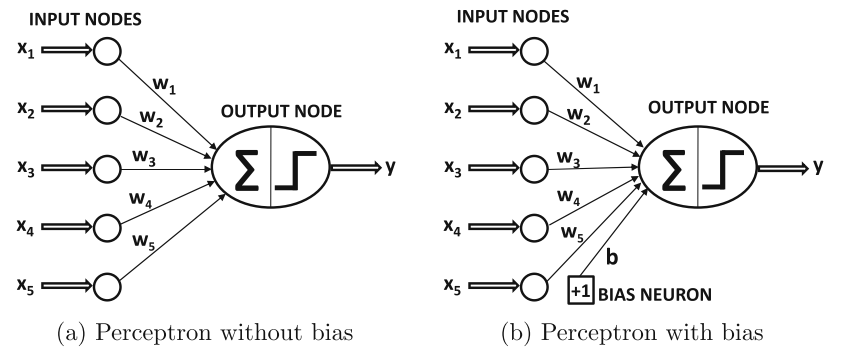
\includegraphics[width=\linewidth]{Figures/fig_perceptron.png}
 \caption{Overview of perceptron architecture. Image extracted from a book~\protect\cite{DBLP:books/sp/Aggarwal18}.}
 \label{fig:perceptron}
\end{figure*} \\
Perceptron is the simplest neural network architecture contains an input layer and output layer which is only a single node. Figure~\ref{fig:perceptron} illustrates a simple perceptron architecture with and without bias neuron. The input layer simply transmits the each individual feature to the output layer by multiplying them with the corresponding weight (e.g., $x_1$ multiplies with $w_1$). Note that since the input layer does not perform any computation, often it is not included in the count of the number of layers in a neural network.

Given a training set where each instance is of a form ($\overline{X}$, $y$) where $\overline{X}=[x_1,x_2,...,x_d]$ denote an input variable with \textit{d}-dimensional features, $b$ is bias and $y$ is an output that $y \in{\{-1, +1\}}$. Let $\overline{W}=[w_1,w_2,...,w_d]$ denote the weight of the edges and the output $\hat{y}$ is computed as follows: \begin{equation}
\hat{y}=sign\{ \overline{W}\cdot \overline{X}+b\} = sign\{ \sum\limits_{j=1}^{d} w_jx_j+b\}
\end{equation}


The sign function maps a real value to either \num{+1} or \num{-1} as $y \in{\{-1, +1\}}$. In other words, the sign function here serves the role of an \textit{activation function}. Depending on the application at hand different type of activation functions such as \textit{logistic regression classifier} can be utilized. The depicted scenario appropriate for binary classification task where the output of the sign function, i.e., \num{-1} or \num{+1} corresponds to a class label. 


The optimization of the perceptron algorithm is performed heuristically and the goal of the algorithm is to minimize the following heuristically motivated loss function with respect to all training instances:

The weights then updated based on the error value as follows:
%Formula 1.3
\begin{equation}
    \nabla L=\sum\limits_{(\overline{X},y) \in D}(y-\hat{y})\overline{X}
\end{equation}
where $D$ denotes the entire training data. Note that the above function is defined over the entire training data. Typically, this type of a neural network is trained by feeding each input data instance $\overline{X}$ one by one to create a prediction $\hat{y}$. Then the weights are updated in each iteration based on the error value $E(\overline{X} = (y-\hat{y}))$ as follows:
%Formula 1.4
\begin{equation}
    \overline{W} \Leftarrow \overline{W} \alpha (y-\hat{y})\overline{X}
\end{equation}
where alfa denoted the learning rate of the neural network. Finally, the weights are updated iteratively until the convergence is reached. 

The introduced perceptron model is a type of linear classifier which defines a linear hyperplane. Therefore, the perceptron model performs well when the data is linearly separable.
%The perceptron algorithm iterates over all the training samples randomly and updates the weights accordingly until convergence is reached.
\subsubsection{Feed Forward Neural Networks}
Feed forward neural networks are multi layer neural networks which contain additional intermediate layers so called \textit{hidden layers} between input and output. The simple architecture of feed forward neural networks is shown in Fig.
In such a network the successive layers feed into one another in the forward direction from input to output. To facilate the discussion first we explain the difference between a shallow neural network and deep neural network. Shallow neural networks contains only one hidden layer and any neural network which contains more than one hidden layer considered as a deep neural network. The given example in Fig is 
a deep feed forward neural network.

\begin{figure*}[h]
\centering
 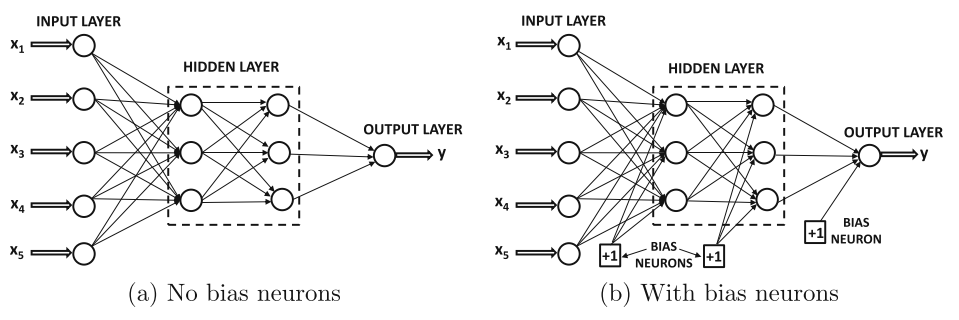
\includegraphics[width=\linewidth]{Figures/fig_ffnn.png}
 \caption{Overview of a simple feed forward neural network architecture. Image extracted from a book~\protect\cite{DBLP:books/sp/Aggarwal18}.}
 \label{fig:perceptron}
\end{figure*}
%In this subsection simple feed forward neural networks (aka shallow neural networks) will be discussed. 

The simple architecture of \textit{3-layer} feed forward neural network (with 2 hidden and output layer) and with/out bias is shown in Fig. %Often the input layer is not counted, The reason of why input layer often not counted because it simply transmits the data without any computation is performed. 
The default architecture of feed forward neural networks (e.g., Fig ) contain a series of fully connected layers, i.e, all the nodes in one layer are connected to those of the next layer. Hence, once the number of layers and nodes in each layer as well as the loss function are defined then the rest of the architecture of the neural network is straight-forward.

Every connection i.e. \textit{edge} between a neuron in a layer and another neuron in the next layer has a weight. Each neuron in all the hidden layers and the output layer gets the input which is the sum of the products of the inputs from the previous layer and respective weights. Further, bias value might also be added to this sum. Then, the activation function is applied to the this sum to produce the output. Note that the number of units in each layer is referred to as the dimensionality of that layer.

Assume the input is \textit{d}-dimensional vector $\overline{x}$ and let $p_1$ denote the number of units in the first hidden layer the weights of the connections between the input layer and the hidden layer are contained in a matrix $W_1$ with size $d\times p_1$. The dimension of the weight matrix $W_r$ between $r$th hidden layer and the $(r+1)$th layer is $p_r\times p_{r+1}$. Finally, assume the output layer contains $o$ nodes, then the final weight matrix is $W_{k+1}$ with a size of $p_k\times o$. Then the input $\overline{x}$ is transformed into the outputs using the following recursive equations~\cite{book}:

\begin{align*}
& \bar{h}_1= \Phi (W_1^{T} \overline{x}) \\
& \bar{h}_{p+1}= \Phi (W_{p+1}^{T} \overline{h}_p), \forall p \in \{1,...,k-1\} \\
& \bar{o}=\Phi (W_{k+1}^{T} \overline{h}_k)
\end{align*}

 \todo[color=green!40]{here explain the formulas e.g., input to hidden }
where $\Phi$ is an activation function like sigmoid. The above equations are general formulation of the forward operation where the given input vectors are transformed into the outputs. It is possible that different layers might use different activation functions, however,  all units in a layer use the same activation function. In such an architecture another common activation functions for the hidden layers is ReLU and for binary outputs is sigmoid function. 
%softmax function outputs with cross-entropy loss for discrete prediction. 
Further, depending on the  goals of the application at hand (e.g., classification or dimensionality reduction), it is possible vary the architecture of the neural network to allow multiple outputs. 

%element-wise fashion to their vector arguments.  some activation functions such as the softmax (which are typically used in the output layers) naturally have vector arguments

%The  arch is shown in Fig explain fig with bias 
%Sin it only transmits the data no computation is performed 


In perceptron the training process is straightforward because the error can be calculate heuristically and the weights updated accordingly. In contrast to perceptron, in the multi-layer neural network the loss is complicated composition function of the weights in earlier layers. For training multi layer neural networks \textit{backpropagation} is a core method which has been widely used to learn such a neural network architecture.
% of learning such a nn architecture.
%backpropagate’ the errors through the layers widely used Backpropagation is a %core method of learning such a nn architecture.
%backpropagate’ the errors through the layers
%widely used algorithm for training feed forward neural networks. 
Such learning process mainly rely on the modification or update of weights and biases during the training process with back propagation. Following Backpropagation algorithm has been very briefly explained and details can be found~\cite{}. 

%In other words, Backpropagation is widely used algorithm for training ffnn. %the learning process in the neurons is simply the modification or update of weights and biases during training with back propagation. 
First we define error function $E(x)$ or cost function which measures the performance of the network as follows:% from other book with y hat
%formula where formulas has no number Introduction to deep learning
\begin{equation}
    E= \frac{1}{2}\sum_{n\in D} (y^{(n)}-\hat{y}^{(n)})^2
\end{equation}


where $n$, $y$, $\hat{y}$ denote the single training sample, target and the output - predicted value of the network, respectively. ... The error function sums error across all the training samples, then the weights are updated accordingly. 

Based on backpropagation the derivative of error function $E$ is taken with respect to $w_i$:
\begin{equation}
    \frac{\partial E}{\partial w_i}=\frac{1}{2}\sum_{n} \frac{\partial y^{(n)}}{\partial w_i} \frac{dE^{(n)}}{y^{(n)}}
\end{equation}

The weight updates are proportional to the error derivations in all training samples and they are added together:
\begin{equation}
    \triangle w_i = - \eta \frac{\partial E}{\partial w_i} = \sum_{n} \eta x_i^{(n)} (y^{(n)} - \hat{y}^{(n)})
\end{equation}
%formula
The details of the derivatives are shown in~\cite{}
Finally, the wights are updated according to the formula below:
%formula page 94
\begin{equation}
   w_{update}= w_{old}-\eta \nabla E
\end{equation}
    
\subsection{Convolutional Neural Networks}
Convolutional neural networks (CNNs) are specialized neural networks for processing grid-structured data, e.g., time series data - 1D grid, image data - 2D grid. Although CNNs can be utilized with various type of data, the majority of the applications are focused on image data. Therefore, in this chapter first general architecture of convolutional neural networks where the input is image data and then application of convolutional neural networks to text categorization task have been described. 

\begin{figure*}[h]
\centering
 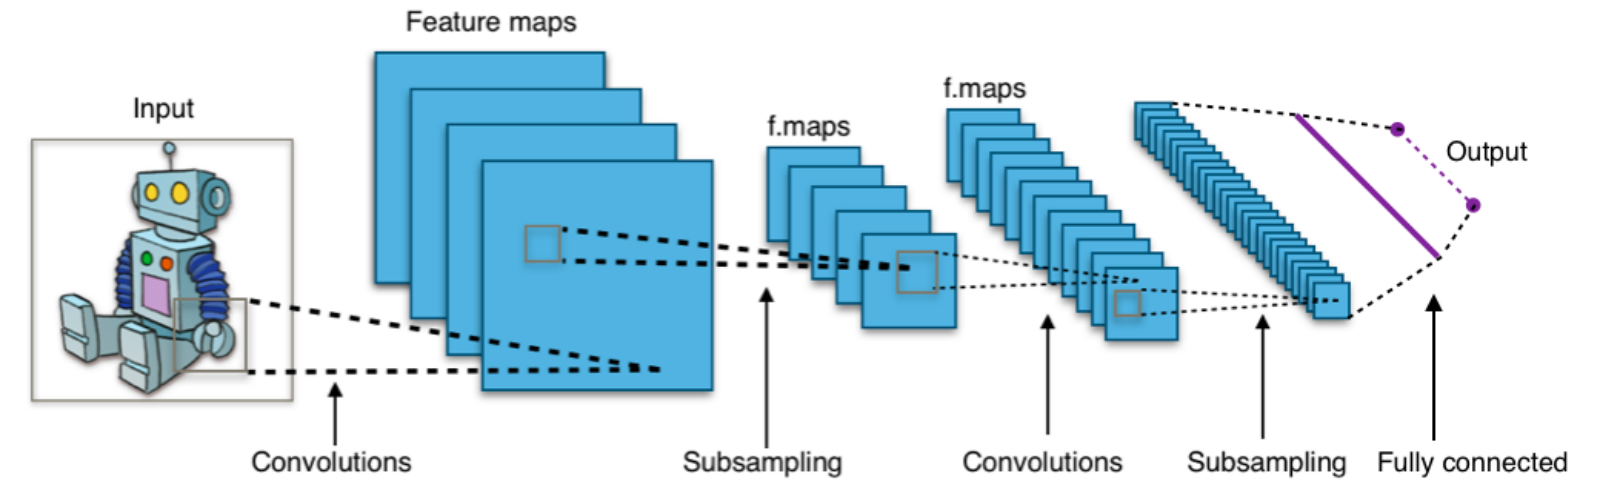
\includegraphics[width=\linewidth]{Figures/fig_cnn.png}
 \caption{Overview of a simple convolutional neural network architecture.}
 \label{fig:perceptron}
\end{figure*}

The convolutional neural networks are similar to the traditional feed forward neural networks, except that the different type of layers are being used. figure depicts basic architectue of a cnn. The most common three layers that present in a standart convolutional neural networks are \textit{convolution}, \textit{pooling},and \textit{ReLU} layer. ReLU is an activation layer which is similarly applied as in the traditional neural networks. Finally, the final layer is often a fully connected layer which maps given inputs into the set of output nodes. Before explaining each layer, first, we examine the input data to the network. As it has already mentioned, we assume that our input is image data. Hence, the input to the convolutional neural network is organized into a 2-dimensional grid structure and each grid value is referred to as \textit{pixels}. Each pixel corresponds to a spatial location within the image. Further, in order to encode the color i.e., red, green, and blue of each pixel multi dimensional array of values at each grid location is being used. Assume that given an image with 32 × 32 spatial dimensions and the depth is 3 , then the overall number of pixels in the image would be 32 × 32 × 3. Moreover, in convolutional neural networks filters or kernels often are organized into 3-dimensional structural units (see Fig. ) which are usually much smaller than those of the layer the filter is applied to. Further, the filter is usually square in terms of its spatial dimension and the depth of it is always same as the layer to which it is applied. 

%intensity of the three primary colors i.e., red, green, and blue then the 
The \textit{convolution operation} places the filter to each possible position in the image and then basically performs the dot product between the filter and the matching grid of the image (which has the same volume with the filter). When performing the convolution operation the filter should be alligned with the filter in way that no portion of the filter is "sticking out" from the borders of the image. The possible dot products defines the dimention of the next layer. The figure illustrates the simple convolution  operation....
%Figure 8.1 or 8.2
\begin{figure*}[h]
\centering
 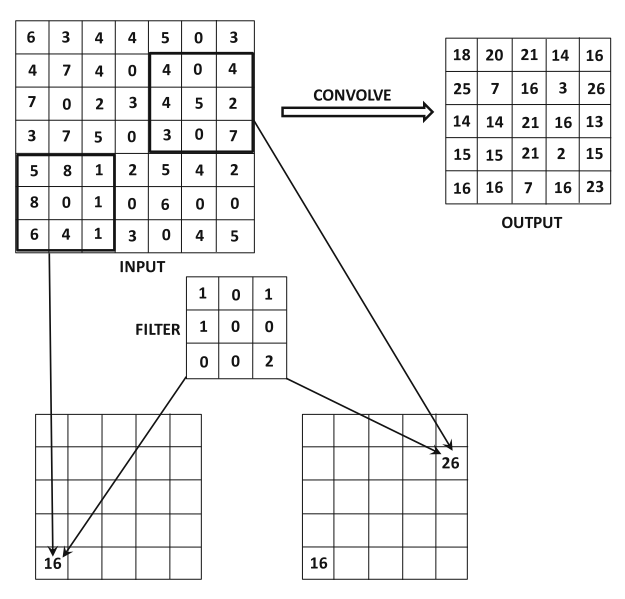
\includegraphics[height=10cm,width=\linewidth]{Figures/fig_cnn_convolution.png}
 \caption{Overview of a simple convolutional neural network architecture.}
 \label{fig:cnn_convolution}
\end{figure*}

The formal definiation of the convolution operation is as folows:

\begin{equation}
\begin{split}
h_{ijp}^{(q+1)} = \sum_{r=1}^{F_q}\sum_{s=1}^{F_q}  \sum_{k=1}^{d_q} w_{rsk}^{(p,q)}h_{i+r-1,j+s-1,k}^{(q)} \forall i \in \{1,...,L_q-F_q +1\}& \\
\forall j \in \{1,...,B_q-F_q +1\}&\\
\forall p \in \{1,...,d_{q+1}\}&
\end{split}
\end{equation}


\subsubsection{Padding}
The convolution operation reduces the size of the (q + 1)th layer in comparison with the size of the qth layer. However, such reduction of the size is not desirable because it tend to cause lose of information.  To avoid such an issue one of the most common way is to use \textit{padding}. In padding operation, first extra added to (Fq \−1)\/2 pixels all around the borders of the feature map, then those pixel values are set to zero as shown in Figure... 

\begin{figure*}[h]
\centering
 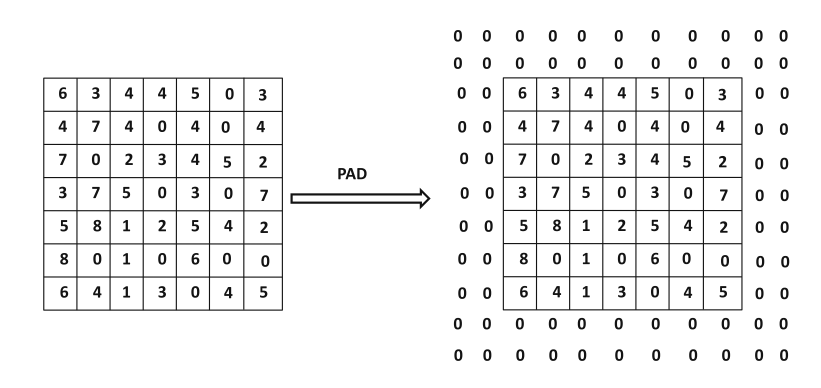
\includegraphics[width=\linewidth]{Figures/fig_cnn_padding.png}
 \caption{Overview of a simple convolutional neural network architecture.}
 \label{fig:cnn_padding}
\end{figure*}

The convolution operation reduces the size of the input volume by (Fq-1). Increasing spatial height and width of the input volume by (Fq-1) with zero padding ensures that the input volume and output volume will have the same size spatially. Since the padded pixel values are zero they do not contribute to the final dot product values. 
%As a result, the convolution operation is performed after pading the input the size of the  
\subsubsection{The ReLU Layer}
The ReLU activation layer is similarly applied as the traditional in a traditional neural network. Often, ReLU layer is not explicitly depicted in architectural representation of the convolutional neural networks. For each of the Lq ×Bq ×dq values in a layer, the ReLU activation function is applied to it to create Lq ×Bq ×dq thereshold values. The dimension of the ReLU applied layer remains the same. Finally, these threshold values are passed to the next layer. %ReLU has a lo of advantages than the other activation functions
\subsubsection{Pooling}
The pooling operation works on a small square grid regions of size Pq x Pq. The pooling operation is performed at the level of each activation map and produces another layer with the same depth. For each square region of size Pq x Pq in an activation map the maximum values are returned and this operation is refered as max pooling. The pooling operation reduces the spatial dimention of the activation map. The example of
\begin{figure*}[h]
\centering
 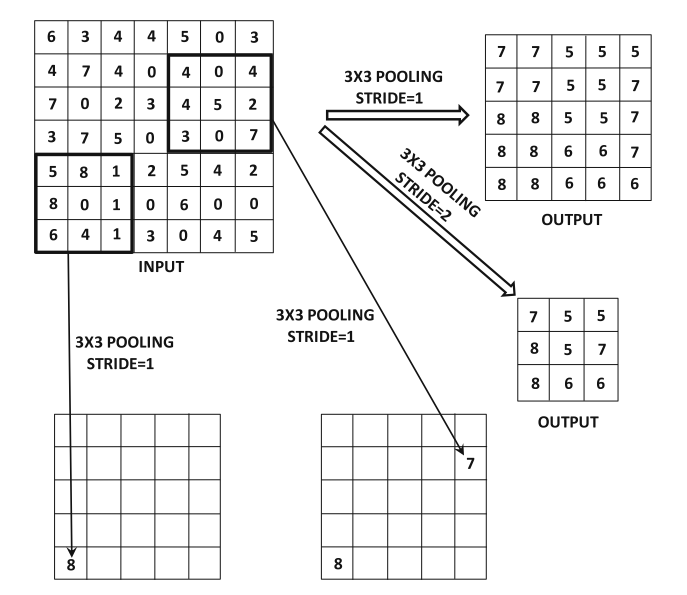
\includegraphics[width=\linewidth]{Figures/fig_cnn_pooling.png}
 \caption{Overview of a simple convolutional neural network architecture.}
 \label{fig:cnn_convolution}
\end{figure*}



There are also other type of pooling such as average-pooling. However, they are rarely used. 
\subsubsection{Fully Connected Layers}
The final spatial layer is connected to a first fully connected layer. This layer is exactly the same as traditional ffnns. Depending on the application at hand the number of the fully connected layers and the activation function output layer  


\subsection{Recurrent Neural Networks}
The recurrent neural networks are derived from  simple ffnn by adding \textit{recurrent} connections on the hidden layer. The rnn can be used in almost any sequential data, however, its use in the text domain is the most common.  
\begin{figure*}[h]
\centering
 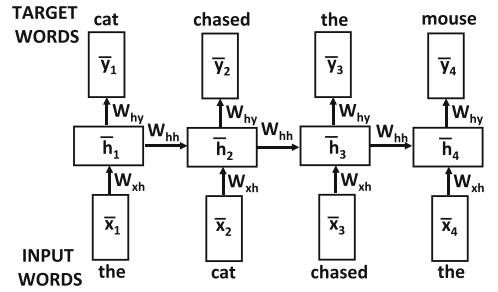
\includegraphics[height=5cm, width=10cm]{Figures/fig_rnn.png}
 \caption{Overview of a simple convolutional neural network architecture.}
 \label{fig:rnn}
\end{figure*}
The simple rnn representation is shown in Figure~\ref{fig:rnn}. This architecture is particularly suited for a language modeling which predicts next word, given the history of the words. One hot coding of words from the given sequence is fed one at a time to the neural network. In other words, this temporal process is same as feeding each word to the inputs at the relevant time-stamps. A time-stamp refers to a position of a word in the sequence. In the given example of a language model the output is a vector of probabilities predicted for the next word. %finish

The input vector at time \textit{t} (e.g., one hot encoded \textit{t}h word of the sequence) is xt, the hidden state is ht and the output yt which is the predicted probabilities of the (t+1)th word. Both input and the output xt and the yt, respectively are d-dimensional vector of a vocabulary of size d. To formulate the entire training processes we consider the simple case in Figure. The hidden state at time \textit{t} as follows:
%formula 7.1
    \begin{equation}
    \overline{h}_t = f(\overline{h}_{t-1},\overline{x}_{t})
\end{equation}
where xt is the input vector and ht-1 is t hidden vector at tme (\textit{t}-1). Further, this function utilizes weight matrices and activation functions. Note that the same weights are used at each time all time-stamps (i.e., sequential elements). 

We define a p×d input-
Why. Then, one can expand Equation 7.1 and also write the condition for the outputs as hidden matrix Wxh,a p × p hidden-hidden matrix Whh,and a d × p h
%formula 7.2
 Here the “tanh” notation is used to denote an activation function, depending on the application at hand different activation functions can be used such as sigmoid,...

The hidden state of the network changes after the input of the each word in the sequence and the weight matrices in different layers are shared to ensure that the same activation function is used at each time-stamp. The particular architecture shown is suited to language modeling. The figure is  language modeling by predicting the next word given the previouse history of words. One hot coding of words are fed one at a time in Fig. relavent time stamp
 

Each time-stamp has an input, hidden unit and output. 

Finally, depending on the application at hand it is possible that input or outputs units to be missing. Example of a sentiment analysis architecture which is a special type of text categorization application is shown in Fig . In sequence classification application such as sentiment analysis we need only one output label which corresponds to the class of the given sequence. 

\subsection{Neural Language Models}
The idea of understanding natural language text data by intelligent systems has been a goal of variety fields in Artificial Intelligent. Hence, it is crucial to represent text data in a form that the machine learning algorithms can process it automatically.  %require a certain representation of text data to be able to process and make sense of it. 
The raw representation of text which consist of set of words cannot be directly processed by the machine learning systems~\cite{srinivasan2017guide}. One of the common ways to represent text is %through 
in a form of a sparse and high dimensional discrete vector. There are several methods such as one hot encoding, bag of words, etc. can be exploited to obtain the such text representations. However, such models have two main disadvantages. First, the dimension of the vectors is high that is specified by the number of words present in vocabulary.  Secondly, to form the vectors the semantic relation between the words are not taken into account.  Besides, such models often lead to inaccurate results on new and rare words. 

%The Vector Space Model (VSM) is one of the most successful and widely used approach to represent text documents~\cite{survey_word_embeddings}. The vector space model originally deveoped for an infomration retriaval system. There are various ways of building VSMs such as ... 
Motivated by the aforementioned challenges of text representations, \textit{word embedding} models have emerged as an important field of research in many NLP tasks~\cite{survey_word_embeddings}. Word embedding models aim to generate low dimensional vector representation of words by preserving syntactic and semantic word relationships. In other words, semantically similar words are placed close to each other in the vector space. Figure~\ref{} illustrates two dimensional projection of word vectors from Skip-Gram which is one of the most prominent word embedding models proposed by . 
\begin{figure*}[t]
 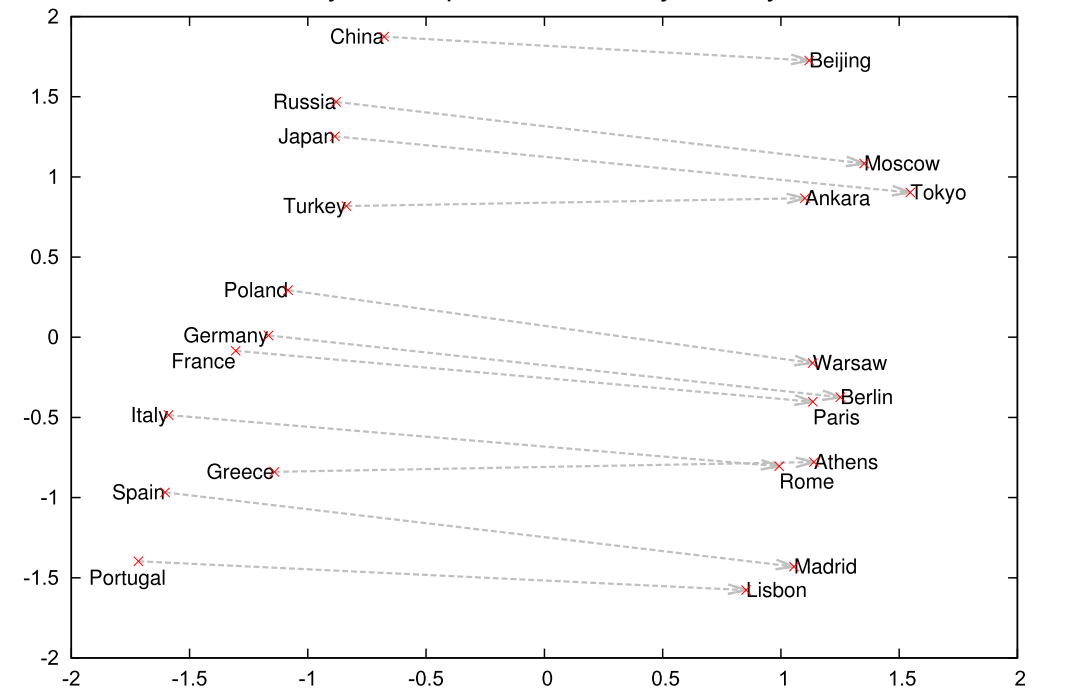
\includegraphics[height=7cm,width=\linewidth]{Figures/fig_word_vec_contries_capitals.png}
 \centering
 \caption{Two dimensional projection of Skip-gram vectors of countries and their capitals. Image extracted from the original paper~\cite{DBLP:conf/nips/MikolovSCCD13}.}
 \label{fig:countries_capitals}
\end{figure*} 
In Figure~\ref{fig:countries_capitals} Skip-gram model is capable of grouping concepts and reflects the implicit relationship, between the words. For example, the distance between countries and capital cities is approximately same or the calculation of vec("Madrid") - vec("Spain") + vec("France") is closer to vec(“Paris”) than to any other word vector~\cite{}. %here there was something  
In addition, the word vectors from the embedding models can be leveraged to construct document vectors. The generated word and/or document vectors then can be utilized in wide range of NLP tasks such as document classification, question answering, sentiment analysis, etc. 

Beside word embedding models, \textit{document embedding} models are proposed to generate the distributed representation of texts, i.e., documents, paragraphs, sentences. The basic idea of these models is that utilizing context word of documents to construct document vectors. \\
In the following, we give an overview of the most prominent word and document embedding models: \\
\begin{itemize}
\item \textbf{PTE~\cite{PTE}.} PTE aims to learn distributed representation of text in a semi-supervised fashion. In other words, PTE leverages both labeled and unlabeled data to learn the representation of documents. Further, unlike other embedding models such as Skip-gram which do not use any labeled data and generalizable for a variety of tasks, PTE designed to be utilized from a particular task.  More precisely, the vector representations can be easily fine tuned for a certain task with a set of labeled dataset. The general workflow of PTE is shown in Figure~\ref{fig:PTE}.
\begin{figure*}[h]
 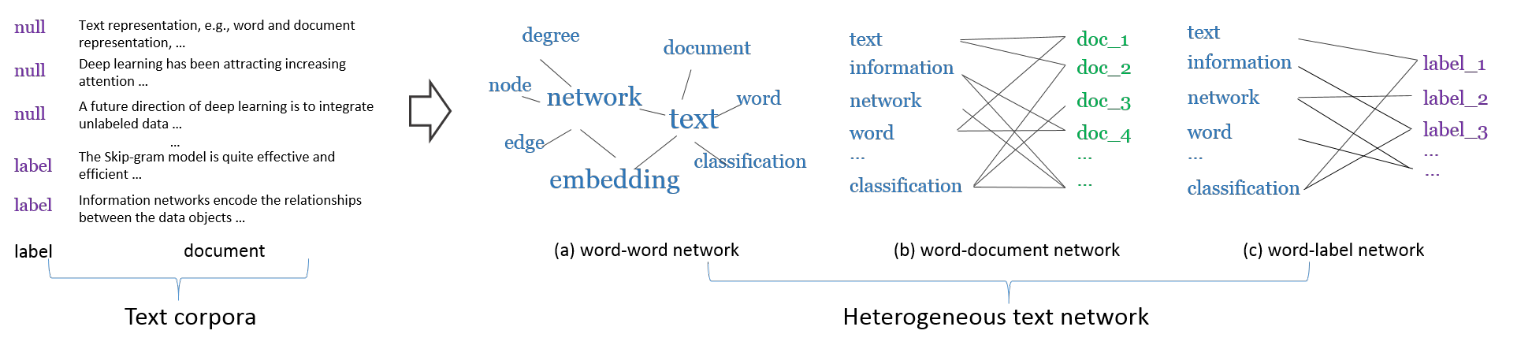
\includegraphics[width=\linewidth]{Figures/fig_PTE.png}
 \caption{Overview of converting text corpora to heterogeneous text network. Image extracted from the original paper~\cite{PTE}.}
 \label{fig:PTE}
\end{figure*} 
Given a large text corpora PTE first encodes the different co-occurrence information of between words-words, words-documents and words-labels. 
Word-word network (see Figure~\ref{fig:PTE}a) captures the co-occurrence of words in the same local context. The weight of the each edge of the network determined by the number of times that two word co-occur in the context windows. Word-document network (see Figure~\ref{fig:PTE}b) encodes the co-occurrence information of words in documents. The weight of an edges between a word and document defined by the number of times the word appears in the document. Word-label network captures the information of category level word co-occurrences. The weight between the word $w_{i}$ and category word $c_{j}$ is $w_{ij}$ which is defined as: $w_{ij} = \sum_{(d:l_{d}=j)} {n_{di}}$ where $l{d}$ is a class label of document $d$ and $n_{di}$ is term frequency of word $v_{i}$. Finally, the combination of word-word, word-document, and word-label networks constitutes the heterogeneous text network. Such network is being exploited by PTE to learn the latent representation of words while preserving the second order proximity (see Section~\ref{subsec:network_embedding_models}).

The overall heterogeneous network consists of three homogeneous networks, i.e., the word-word, word-document and word-label networks. PTE~\cite{PTE}, to embed each of these networks, aims to capture the second order proximity~\cite{tang2015line}.
To model the second-order proximity of a homogeneous network, for each edge $(v_i,v_j)$, the conditional probability $p(v_{j}|v_{i})$ is defined as follows~\cite{tang2015line}: 
\begin{equation}
%p(v_{j}|v_{i})=\frac{exp(-\vec{u}_{j}^{T}\cdot\vec{u}_{i})}{\sum\limits_{k=1}^{|V|} exp(-\vec{u}_{k}^{T}\cdot\vec{u}_{i})}\,,
p(v_{j}|v_{i})=\frac{exp(-\vec{u}_{j}^{T}\cdot\vec{u}_{i})}{\sum\limits_{v_k\in V} exp(-\vec{u}_{k}^{T}\cdot\vec{u}_{i})}\,,
%\raisepunct{,}
%p_{1}(v_{j}|v_{i})=\frac{exp(-\vec{u}_{i}^{T}.\vec{u}_{j})}{\sum_{k=1}^{V}exp(-\vec{u}_{i}^{T}.\vec{u}_{j})}
\end{equation}
where $V$ is the set of vertices connected with $v_i$ in the network, $\vec{u}_{i}$, $\vec{u}_{j}$ and $\vec{u}_{k}$ are the vectors of vertices $v_i$, $v_j$ and $v_k$, respectively. The empirical probability of $p(v_{j}|v_{i})$ can be defined as $\hat{p}(v_j|v_i)=\frac{w_{ij}}{d_i}$, where $d_i$ is the out-degree of $v_i$ and $w_{ij}$ is the weight of the edge $(v_i,v_j)$.

In order to preserve the second-order proximity, the conditional distribution $p(v_{j}|v_{i})$ is made close to $\hat{p}(v_{j}|v_{i})$ based on the KL-divergence over the entire set of vertices in the network, such that the model minimizes the following objective function:
\begin{equation}\label{optimizationHomo}
O=-\sum_{(v_i,v_j) \in E}w_{ij} \textrm{log} \,(p(v_{j}|v_{i}))\,,
\end{equation}

The embedding of the individual word-word, word-document and word-label networks are learned simultaneously by minimizing the following objective function:
% $O={O}_{ee}+{O}_{ec}$ .
 \begin{equation}\label{optimizationHet}
 O_{pte}={O}_{ww}+{O}_{wd}+{O}_{wl}\,,
 \end{equation}

where ${O}_{ww}$, ${O}_{wd}$ and ${O}_{wl}$ are the objective functions defined in Eq.~(\ref{optimizationHomo}) for the homogeneous word-word, word-document and word-label networks, respectively. 
To optimize the objective function in Eq.~(\ref{optimizationHet}), the edges are firstly collected from these three homogeneous networks as three sets, one for word-word edges, one for word-document edges and the other for word-label edges, and then in each training iteration, edges are sampled from each set to update the model. Readers can refer to~\cite{PTE,LINE}, for the detailed optimization process.

Once the word vectors are learned then the  representation of an arbitrary piece of text i.e., words $w_1, w_2, w_3,..., w_n$ present in text $d$ is simply inferred as the average of the word representations as follows:

\begin{equation}
\vec d= \frac{1}{n}\sum_{i=1}^{n}\vec u_{i}.
\end{equation}

\item \textbf{Skip-gram~\cite{DBLP:journals/corr/abs-1301-3781}.} Skip-gram model learns the low dimensional representation of words while capturing syntactic and semantic word relationships from a given large corpus. The word vectors are computed leveraging 2-layer simple feed forward neural networks. Training Skip-gram is very efficient, i.e., depending on the size of the corpus and the parameters it can only take couple of hours. Moreover, the model can be easily adapted to domain specific applications, e.g., patent classification by training it with a relevant large text corpus.
The Figure~\ref{fig:skip_gram} depicts the overview of Skip-gram model. 
\begin{figure*}[h]
\centering
 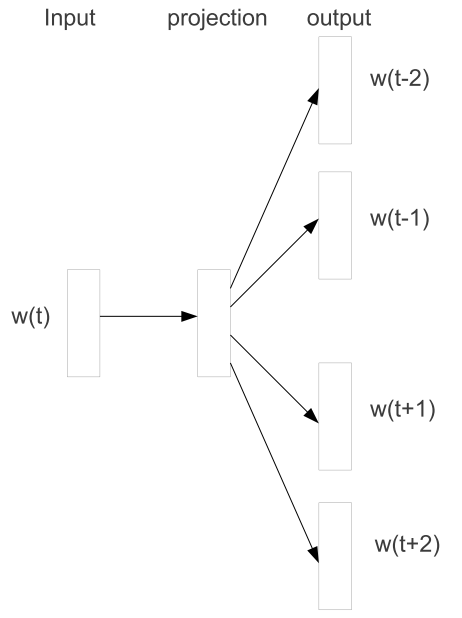
\includegraphics[height=4cm,width=4cm]{Figures/fig_skip_gram.png}
 \caption{Overview of Skip-gram model architecture. Image extracted from the original paper~\cite{DBLP:journals/corr/abs-1301-3781}.}
 \label{fig:skip_gram}
\end{figure*} \\
The basic idea of the model is to given a word  $w(t)$ from a sentence, the model tries to predict the  probability for every word in the vocabulary of being the \textit{nearby word}, i.e., window of surrounding context words. According to Figure~\ref{fig:skip_gram}, surrounding context words of $w(t)$ are $w(t-2), w(t-1), w(t+1), w(t+2)$. Note that the size of the window is an input parameter. %Ideally, the actual nearby words should have the higher probability than the other 

The objective of the training Skip-gram model is to compute word vectors that are useful for predicting the surrounding words in a text. Then the objective of Skip-gram model is to maximize average log probability a given sequence of words $w_1, w_2, w_3, ..., w_T$ as follows: 

\begin{equation}
\frac{1}{T}\sum_{t=1}^{T}\sum_{-c \leq j\leq c, j\neq0 } \textrm{log} p(w_{t+1}|w_{t})
\end{equation}
where $c$ is the size of the training context and specified with the window size. The higher the window size more the training samples are. \\
The probability $p(w_{t+1}|w_{t})$ defined by using softmax function: 
\begin{equation}
p(w_{O}|w_{I})=\frac{exp({v^{'}_{w_O}}^{T} {v}_{w_{I}})}{\sum\limits_{w=1}^{W} exp({v^{'}_w}^{T} {v}_{w_{I}})}
\end{equation}
where $v_w$ and $v'_w$ are input and output vector representation of $w$, and $W$ in the number of entire words in the vocabulary. Computing such an equation for each training sample is a very expensive task. Therefore, instead of calculating full softmax, hierarchical softmax which is computationally much more efficient is being used. Unlike softmax which evaluates $|W|$ output nodes to find the probability distribution, hierarchical softmax evaluates only approximately $\textrm{log}_2(W)$ nodes. The output layer is represented as a binary tree in Hierarchical softmax. Each leaf node corresponds to a word $w$, $w \in W$. For each node the tree relatively represent the probability of its child node(s). The hierarchical softmax defined as follows:

\begin{equation}
\displaystyle P(w|w_I) \prod_{j=1}^{L(w)-1} \sigma([n(w,j+1)=ch(n(w,j))]\cdot {v^{'}_{n(w,j)}}^{T} {v}_{w_{I}} )  
\end{equation}
where $n(w,j)$ is $j$-th node on the path from the root to $w$, $L(w)$ is the length of this path and $\sigma(x)=1/(1+exp(-x))$. Given the equation of hierarchical softmax the cost of computing $P(w|w_I)$ is on average not greater than $\textrm{log}W$.

Furthermore, the authors simply Noise Contrastive Estimation (NCE)~\cite{cite} method as alternative to the hierarchical softmax. NCE is based on the idea that a successful should be capable of differentiation data from the noise with the help of logistic regression model. Then for the Skip-gram model  the goal is to given a $P(w_O|w_I)$ distinguish between the target word $w_O$ and the negative samples which are drawn randomly. For each data sample there are $k$ negative samples. Then the objective of Negative sampling defined as follows: 
\begin{equation}
 \textrm{log}\sigma({v^{'}_{w_O}}^{T} {v}_{w_{I}} )+ \sum_{i=1 }\mathbb{E}_{w_i\sim P_n(w)}\left[ \textrm{log}\sigma({- v^{'}_{w_O}}^{T} {v}_{w_{I}} ) \right] 
\end{equation}
where $P_n(w)$ is noise distribution from which the negative samples are drawn. $P_n(w)$ is a parameter which authors show that the uniform distribution performs the best for several tasks.

The Skip-gram models requires large corpora for learning the vector representation of words and the frequency of words has impact on the quality of the vectors. In very large corpora, usually the most frequent are the least informative words (e.g., "the", "a", "an", "up"). To address this problem a simple subsampling approach has been defined as:
\begin{equation}
P(w_i)=1-\sqrt{\frac{t}{f(w_i)} }
\end{equation}
where $f(w_i)$ is the frequency of word $w_i$ and $t$ is a chosen threshold, around $10^{-5}$. 

Overall, the Skip-gram model has been the base of many embedding models such as DeepWalk, node2vec, doc2vec etc. In addition, it is still one of the most standard baselines for many word, document and network embedding models.\\\todo{here you can explain word2vec model in 2 variations, i.e, skip-gram and cbow.}
% two-layer neural networks
%look at the words nearby and pick one at random. The network is going to tell us the probability for every word in our vocabulary of being the “nearby word” that we chose.

% and CBOW
\begin{figure*}[t]
\centering
 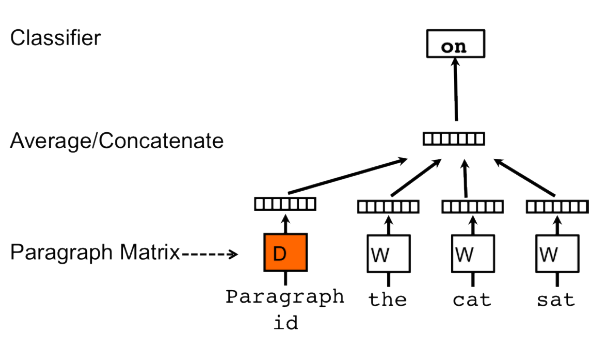
\includegraphics[height=5cm,width=8cm]{Figures/fig_doc2vec.png}
 \caption{Overview of doc2vec model architecture. Image extracted from the original paper~\cite{DBLP:conf/icml/LeM14}.}
 \label{fig:doc2vec}
\end{figure*} 
\item \textbf{Doc2vec~\cite{DBLP:conf/icml/LeM14}.}
Doc2vec model extends Skip-gram model in order to obtain latent representation of texts  i.e., sentences, paragraphs, documents. Unlike Skip-gram which learns only the vector representation of words from large corpora, doc2vec learns vector representation of words as well as the documents (in which the words present).  Doc2Vec is an unsupervised algorithm which is trained to to be useful for predicting the words in documents to learn the document representations. Therefore, semantically similar documents or documents that share many common words expected to be located close to each other in the common vector space. 
The Figure~\ref{fig:doc2vec} illustrates the overview of doc2vec architecture. The document vector $D$ is concatenated (or averaged) with the word vectors $W$ from the document, then the model predicts the following word in the given context.

The model is inspired by the Skip-gram architecture, which is trained to predict a word given context words. The doc2vec models is also trained to predict next word from given context information. However, in doc2vec the input is not only words but also a document vector which is treated similar to the word vectors. Every word and every document from the given corpora mapped to unique vector. After the training word as well as document vectors can be used in wide range of NLP task such as text classification, question answering, text summarization etc. Since the architecture of doc2vec is very similar to Skip-gram, we do not discuss the technical details here. \\   

%\item \textbf{ELMo.}\\
\item \textbf{BERT~\cite{DBLP:conf/naacl/DevlinCLT19}.} Bidirectional Encoder Representations from Transformers (BERT) is a language representation model which utilizes both jointly right and left context in all layers to pretrain deep bidirectional representations. The pretrained model then can be easily fine tuned to create language representation model for wide range natural language processing tasks. The technical implementation of BERT almost identical to the previous study by .... therefore, here we skip the technical details of the model.
The framework of BERT is shown in Figure~\ref{fig:bert}.
\begin{figure*}[h]
\centering
 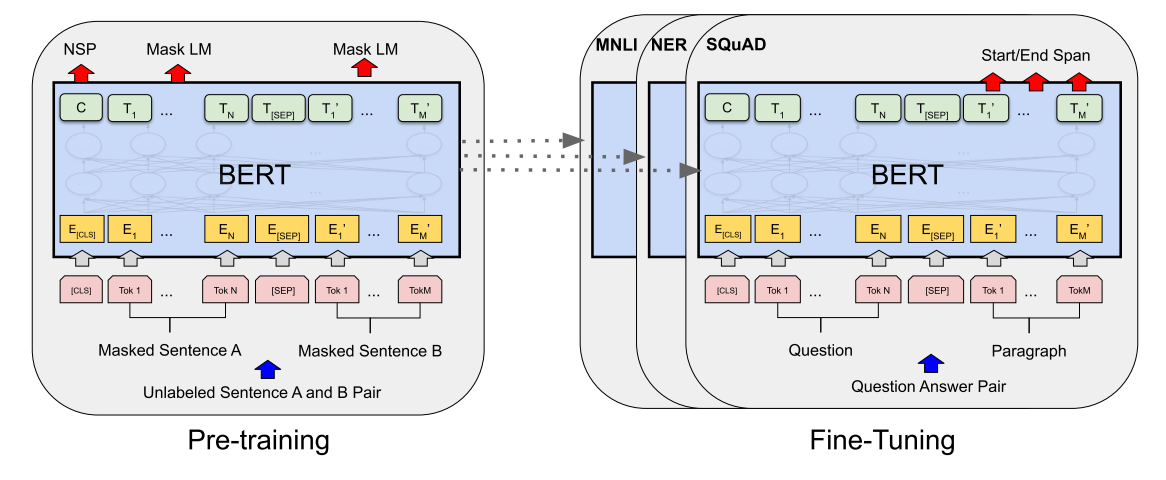
\includegraphics[width=\linewidth]{Figures/fig_BERT.png}
 \caption{Overview of BERT architecture. Image extracted from the original paper~\cite{DBLP:conf/naacl/DevlinCLT19}.}
 \label{fig:bert}
\end{figure*} 

BERT framework consists of two main steps (see Figure~\ref{fig:bert}) namely, pre-training and fine-tuning. Input to BERT is sequence of words which can be a single sentence or a pair of sentences. The first token of every input is always a special token ([CLS]) and the pair of sentences are separated by another special token ([SEP]). The input embedding of each token denoted as $E$ and the final hidden vector for the $i^{th}$ input token as $T_i$. \\
During the pre-training phase which is illustrated left part of Figure~\ref{fig:bert}, model is trained with two unsupervised tasks, namely, masked language modeling and next sentence prediction.
Masked language model task randomly masks some tokens of the input, then predicts those masked tokens. In this task, the final hidden vectors of masked tokens are fed into an output softmax over the vocabulary. Overall, the model tries to predict the masked inputs instead of an entire input.\\
The second task of pre-training is binarized next sentence prediction (NSP). The goal of the task is to train the model to learn the relationship between two sentences. In order to train the model, the dataset generation phrase is straightforward. Given a sentence A and if the sentence B is the actual next sentence that follows A then labelled as IsNext and the randomly selected sentences from the corpus would be labeled as NotNext. As shown in Figure~\ref{fig:bert}, $C$ which is the final hidden vector of the special token ([CLS]) is used for next sentence prediction task.\\
The second component of the frame work is fine-tuning as shown in Figure~\ref{fig:bert} (right). After the pre-training phase, all the parameters of the model can be fine-tuned with labeled data. In other words, depending on the application at hand such as question answering task, inputs and outputs, i.e., question-passage pairs are plugged into BERT in order to fine tune all the parameters. Note that  for each application at hand there are different fine-tuned models. 


\end{itemize}

%PTE
%CBOW, Skip-Gram
%ELMo , GPT , BERT
%doc2vec
%
\subsection{Network Embedding Models}
\label{subsec:network_embedding_models}
Networks are powerful structures for modeling many sophisticated systems such as information networks, social networks, etc. To be able to process the network data for variety of tasks such link prediction, node classification, node clustering etc. effective and efficient representation of the network data is crucial. The traditional explicit network representation methds such as adjency matrixes\todo{check} seem to be quite inefficient in large-scale networks. Motivated by this challenge several network emdedding models have been proposed~\cite{}.
Network embedding models are designed to generate the low dimensional vector representation of nodes based on the assumption that the structure of the network should be reflected in the learned feature representations. The relation of the nodes in the network, i.e., the connection between the nodes preserved also in the vector space as well. In other words, nodes that are considered to be similar based on the structure of the network should be placed closely in the vector space where similarity is measured by the distance between the nodes. 
Figure~\ref{karate} illustrates an example of an embedding model. Given the input karate network (Figure~\ref{}b) the similar nodes (that share the same color) placed close to each other in the embedding space (Figure~\ref{}b). The network embedding model aims to preserve the network structure while learning the dense and continuous representations of nodes in a low dimensional space. 
Traditionally, a network is represented as graph, hence following first we give the formal general definition of a Graph and then network embedding task.
\begin{definition}{(Graph):\\}
\textit{A $G(V, E)$ contains a set of vertices $V={}$ and set and a set of edges $E={}$ where E ⊆ (V × V).}
\end{definition}

\begin{definition}{(Network embedding):\\}
\textit{A network embedding function $f : V \rightarrow $ which maps each vertix $v \in V$ to  $d$ dimentional vector in Rd }
\end{definition}

There are two main goals that network embedding models aim to achieve in order to represent the nodes in a low dimensional space~\cite{survey}: (1) The original network can be reconstructed from the learned vector space, in other words, nodes that connected in the original network should be distance between them should be small. (2) The learned embedding space should be applicable to original network inference task such as identifying important nodes.

Moreover, to embed the nodes of a network into common vector space, different network embedding models adopt different approaches, i.e., matrix factorization, random walk, deep neural networks, etc. In this section we discuss the most commonly used approaches:  
\begin{itemize}
\item \textbf{Matrix Factorization.}\\
To represent a network topology matrices~\cite{survey} where each row and colom corresponds to a node are commonly used. Each entry in this matrix indicates the relation between the corresponding nodes. Network embedding models aim to find the low dimentional representation of nodes of the given network. Matrix factorization methids are common ways to achieve this purpose. Matrix factorization can be Given a matrix M  
%sepNE formula 1
\item \textbf{Random Walk.}\\
Random walks have been used in variety of applications such as .. as a similarity measure~\cite{deewalk}. In the context of network embeddings, random walk models are being exploited to generate random paths over a given network. By doing so, neighbourhood information of vertices can be extracted from the network. Network embedding models which exploit random walk techniques mainly relies on the neighbourhood information of vertices in order to generate vector representation of vertices. This idea highly relates to a neural language model by regarding a vertex as a word and a random walk is a sentence then the node neighborhood can be identified by co-occurence rate as in Skip-Gram model~\cite{survey}.   

\end{itemize}
Furthermore, deep neural networks are also commonly exploited by the several network embedding models~\cite{}\todo{find embedding models as an example}. Neural networks have been discussed in Section~\ref{secnn}.   


In the following we give the example of the most prominent network ebedding models applications:
\begin{itemize}
%cite each of them
\item \textbf{DeepWalk.}
DeepWalk network embedding model aims to learn distributed representation of the vertices in a given network by considering the neighborhood relations of vertices. To this end, the model attempts to conduct two main tasks; first, the model generates random walks on a given network and secondly, the representation of each vertex which is generated by the random walks (from the first step) is updated based on a neural language model. More precisely, DeepWalk relates the distribution of each vertex appearing in random walks to the distribution of words that appear in natural language~\cite{DBLP:journals/tkde/CuiWPZ19}. Motivated by this assumption, DeepWalk adapts a language model so called Skip-Gram to update the representation of each vertex generated by the random walks.
\begin{figure*}[h]
 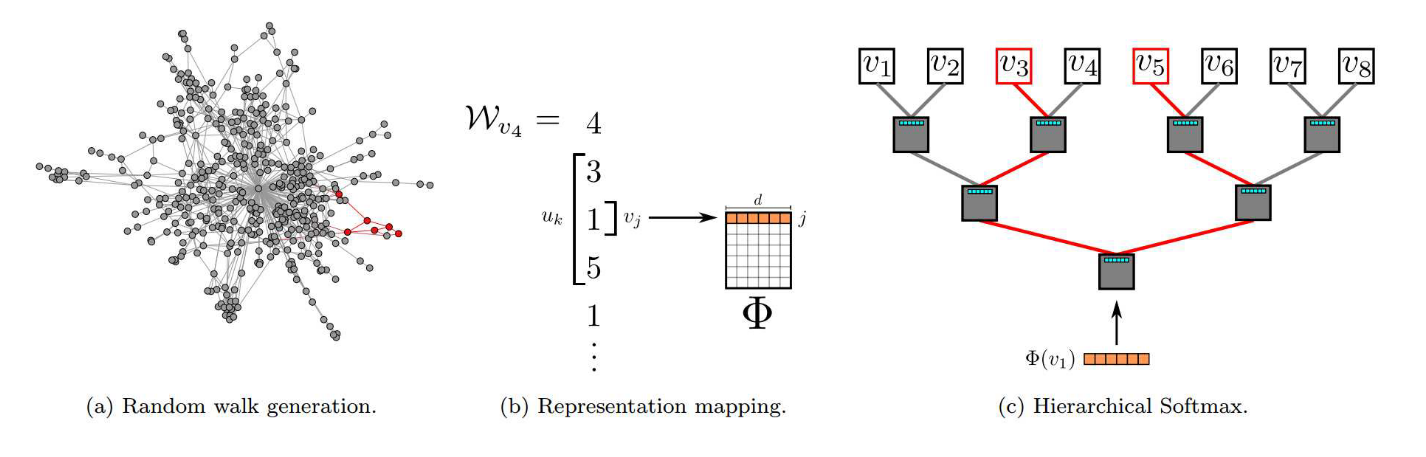
\includegraphics[width=\linewidth]{Figures/fig_deepwalk.png}
 \caption{Overview of DeepWalk. Image extracted from the original paper~\cite{}.}
 \label{fig:deepWalk}
\end{figure*} \\
Figure~\ref{fig:deepWalk} depicts the overview of the DeepWalk model. Given a graph the random walk generator (Figure~\ref{fig:deepWalk}a) randomly samples uniformly a vertex $v$ as a root of the random walk $W$. Then the walk uniformly samples the neighbour of the last visited vertex iteratively until the maximum length of the walk $t$ is reached. The maximum length of the walks ($t$) is an input parameter. Likewise, the number of walks at each vertex $\gamma$ is also an input parameter.\\ 
Skip gram model iterates over all collocation of vertices that appear within the given window size. In Section we have already \todo{Skip gram section, also check SkipGram vs Hsoftmax} introduced the Skip gram model, therefore, in this section we skip the technical details of it. As shown in Figure~\ref{fig:deepWalk}b each vertex $v$ is mapped to its current representation vector $\Phi(v)$. Finally, Hierarchical Softmax is used to learn the distributed representation of the vertices. \\
 
\item \textbf{LINE.}
Large-scale Information Network Embedding (LINE) learns latent representation of vertices of an arbitrary, i.e., undirected, directed, and/or weighted type of an information network. The model is capable of scaling to very large information networks. Moreover, LINE aims to optimize an objective function which preserves the local structure, i.e., \textit{first order proximity} and global structure, i.e., \textit{second order proximity} of a given network. 
\begin{figure*}[h]
\centering
 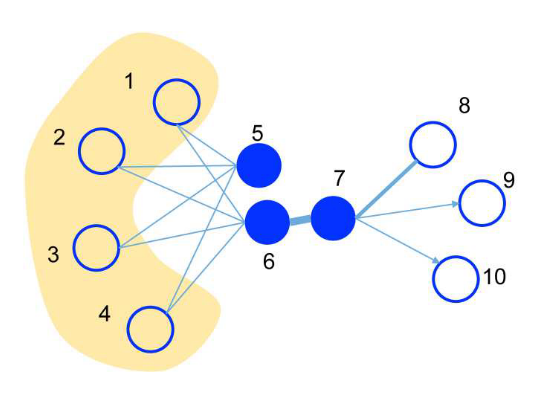
\includegraphics[height=5cm]{Figures/fig_LINE.png}
 \caption{An example of an information network. Image extracted from the original paper~\cite{LINE}.}
 \label{fig:LINE}
\end{figure*} \\
Figure~\ref{fig:LINE} illustrates an example of a simple information network. The thickness of the edges between vertices determines the strongness of the connections. 
First order proximity defined as the observed local pairwise proximity between two nodes~\cite{DBLP:journals/tkde/CuiWPZ19}. For example, in Figure~\ref{fig:LINE} the observed edge between vertex 6 and 7 is stronger, i.e., thicker. According the first order proximity vertex 6 and 7 should be placed closely in the vector space. On the other hand, the first order proximity between the vertex 5 and 6 is zero as there is no edge between them.
To model the first order proximity between vertices $v_i$ and $v_j$ the following joint probability defined as:
\begin{equation} \label{eq:jointProb}
p_{1}(v_{i},v_{j})=\frac{1}{1+exp(-\vec{u}_{i}^{T}\cdot\vec{u}_{j})}
\end{equation}
where $\vec{u}_{i}$ ($\vec{u}_{j}$) is the vector representation of node $v_i$ ($v_j$), respectively. In addition, its empirical probability can be defined as $\hat{p_1}(v_i,v_j)=\frac{w_{ij}}{W}$, where $W=\sum_{(i,j) \in E}w_{ij}$, $E$ is the set of edges between nodes in the network, and $w_{ij}$ is the weight of the edge $(i,j)$.
In order to preserve the first-order proximity, the model aims to minimize the KL-divergence between the two distributions $p_{1}(v_{i},v_{j})$ and $\hat{p_1}(v_i,v_j)$. By omitting some constants, the final goal is to minimize the following objective function:
\begin{equation}
O_{1}=-\sum_{(i,j) \in E}w_{ij} \textrm{log}p_{1}(v_{i},v_{j})
\end{equation}
Note that the first order proximity only applicable for the undirected graphs.

Second order proximity is determined between the two vertices through the shared neighborhood structures of the vertices. In other words, two nodes considered to be similar if they share the same neighbors according to the notation of second order proximity. For example, the vertex 5 and 6 in Figure~\ref{fig:LINE} should be placed closely as they share similar neighbors. 
To model the second-order proximity, for each edge $(i,j)$, the conditional probability is defined as follows: 
\begin{equation}
p_{2}(v_{j}|v_{i})=\frac{exp(-\vec{u}_{j}^{T}\cdot\vec{u}_{i})}{\sum\limits_{k=1}^{|V|} exp(-\vec{u}_{k}^{T}\cdot\vec{u}_{i})}
%p_{1}(v_{j}|v_{i})=\frac{exp(-\vec{u}_{i}^{T}.\vec{u}_{j})}{\sum_{k=1}^{V}exp(-\vec{u}_{i}^{T}.\vec{u}_{j})}
\end{equation}
where $V$ is the set of nodes connected with $v_i$ in the network. The empirical probability of $p_{2}(v_{j}|v_{i})$ can be defined as $\hat{p_2}(v_{j}|v_{i})=\frac{w_{ij}}{d_i}$, where $d_i$ is the out-degree of $v_i$. In order to preserve the second-order proximity, the conditional distribution $p_{2}(v_{j}|v_{i})$ is made close to $\hat{p_2}(v_{j}|v_{i})$ based on the KL-divergence over the entire set of nodes in the network, such that the model minimizes the following objective function:
\begin{equation}
O_{2}=-\sum_{(i,j) \in E}w_{ij} \textrm{log} p_{2}(v_{j}|v_{i})
\end{equation}

In order to keep both first-order and second-order proximities for each node, two LINE models are trained. Firstly, a LINE model is trained by preserving the first-order proximity, and then another LINE model is trained by preserving the second-order proximity. Finally, concatenating the embeddings of both models yields an embedding for each node. \\

\item \textbf{Node2vec.}
Scalable Feature Learning for Networks (node2vec) model is based on the idea of learning the latent representation of the vertices in a given network by maximizing the likelihood of preserving network neighborhoods of vertices. Node2vec extends a prior work, i.e., DeepWalk, which is based on rigid notions of network neighborhoods. Unlike DeepWalk, node2vec designs a biased random walk procedure which explores diverse neighborhoods.  In other words, node2vec leverages \nth{2} order random walk approach to generate neighbourhoods for vertices\todo{nodes or vertices}. The key contribution of the model is biased random walk strategy which is capable of exploring diverse neighbours of vertices.\\  
Given a network $G = (V, E)$ where $V$ is all the vertices and $E$ is all the edges between the vertices in the network. Let $f : V \to \mathbb{R}^d$ be the function that maps the each vertex to its corresponding distributed $d$ dimensional vector representation. For each source node (the start node of a random walk) $u\in V$ , $N_s(u) \subset V$ is defined as network neighborhood of $u$ generated by biased random walk strategy $S$.\\
$S$ generates biased random walks in order to sample the neighborhood nodes that smoothly interpolate between breadth-first sampling (BFS) and depth-first sampling (DFS). 
Then, given a source node $u$ and the length $l$ of the walk, $c_i$ the $i_{th}$ node in the walk generated by the following distribution:


\begin{equation}
    P(c_i = x| c_{i-1}=v )= \begin{cases}
    \frac{\pi_{vx} }{Z}, & \text{if $(v,x)\in E$}.\\
    0, & \text{otherwise}.
  \end{cases}
\end{equation}

where $c_0 =u$, $\pi_{vx}$ is the transition probability between nodes $v$ and $x$, and $Z$ is the normalization constant. \\
Assuming a random walk traversed edge $(t, v)$ and now resides at node $v$. For the next step, the walk evaluates the transition probabilities on edges $(v,x)$ leading from $v$. Then the transition probability $\pi_{vx}=\alpha_{pq}(t,x)\cdot w_{vx}$ can be set as follows:
\begin{equation}
    \alpha_{pq}(t,x)= \begin{cases}
    \frac{1}{p}, & \text{if $d_{tx}$=0}.\\
    1, & \text{if $d_{tx}$=1}.\\
    \frac{1}{q}, & \text{if $d_{tx}$=2}.\\
  \end{cases}
\end{equation}
where $d_{tx}$ denotes the shortest path distance between nodes $t$ and $x$. The parameter $p$ controls the likelihood of immediately revisiting a node in the walk whereas $q$ allows the search to differentiate between inward and outward nodes.%“inward” and “outward” nodes.

Finally, the model tries to optimize the following objective function as follows:
\begin{equation}\label{eq:node2vec_objective}
\max_{f} \sum_{u \in V } \textrm{log} Pr(N_S(u)|f_{u})
\end{equation}

which maximizes the log-probability of observing a network neighborhood $N_S(u)$ for a node $u$ conditioned on its feature representation, given by $f$.\\
In order to optimize the above objective function two assumptions are made as:
\begin{itemize}
\item The likelihood of observing a neighborhood node is independent of observing any other neighborhood node as:
\begin{equation}
 Pr(N_S(u)|f(u))= \prod_{n_i \in N_S(u)}Pr(n_i|f(u))
\end{equation}
\item A source node and neighborhood node have a symmetric effect over each other in feature space and this assumption modeled as follows:

\begin{equation}
P_{r}(n_{i}|f(u))=\frac{exp(f(n_i)\cdot f(u))}{\sum\limits_{v \in V} exp(f(v)\cdot f(u))}
%p_{1}(v_{j}|v_{i})=\frac{exp(-\vec{u}_{i}^{T}.\vec{u}_{j})}{\sum_{k=1}^{V}exp(-\vec{u}_{i}^{T}.\vec{u}_{j})}
\end{equation}

\end{itemize}
Finally with the two above assumptions the Equation~\ref{eq:node2vec_objective} simplifies as follows:
\begin{equation}\label{eq:node2vec_objective_final}
\max_{f} \sum_{u \in V }[ -\textrm{log}Z_u + \sum_{n_i \in N_S (u) }f(n_i) \cdot f(u)]
\end{equation}
where $Z_u$ is a per\_node partition function which is $Z_u= \sum\limits_{v \in V} exp(f(v)\cdot f(u))$. The partition function $Z_u$ is expensive to calculate especially for the large networks, therefore, similar to Skip-gram model negative sampling method is adapted to approximate $Z_u$ function and stochastic gradient ascent is used to optimize the Equation~\ref{eq:node2vec_objective_final}.\\

%As it can be seen from the objective function~\ref{Equation 1} of the model is an extension of 
%Skip gram model. However, the neighbourhood sampling method $S$  is the key contribution of the model which generates biased random walks in order to sample the neighborhood nodes that smoothly interpolate between breadth-first sampling (BFS) and depth-first sampling (DFS). 

\item \textbf{SepNE.}
Given a network SepNE model learns the latent representation of vertices in subsets and in separeta processes. By doing so the model avoids the effort to embed the nodes that are irrelevant to the application at hand. Therefore, the model is capable of scaling to very large networks.\\
\begin{figure*}[h]
\centering
 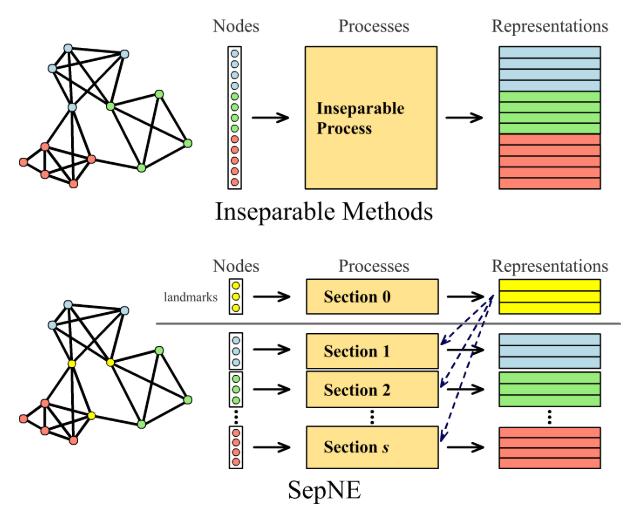
\includegraphics[height=5cm]{Figures/fig_SepNE.png}
 \caption{An example of Inseparable and separable network embedding processes. Image extracted from the original paper.}
 \label{fig:SepNE}
\end{figure*} \\
Figure~\cite{SepNE} depicts simple framework of SepNE and other models that do not separate the learning process. Traditional embedding models such as DeepWalk, LINE, node2Vec embed entire networks with inseparable processes. Unlike aforementioned models SepNE first, partitions the entire network into small subsets of nodes as shown in Figure~\ref{fig:SepNE}. A special set so called \textit{landmark set} which contains the highly interactive nodes in the network is constructed. The goal of the landmark set is to help for establishing references for different sets. First the landmark nodes are embedded, then the rest of the subsets are also embedded.\\
The model is formalized based on \textit{separated matrix factorization} (SMF). Let us firs briefly explain matrix factorization (MF) . Given a matrix $M$ which is of size $(nxn)$, matrix factorization aims to reduce $M$ into its constituent parts $W$ and $C$ that both $W$ and $C$ satisfy given constraints in Equation~\ref{mf} for reconstructing $M$. On the other, separated matrix factorization takes a network $G=(V,E)$ its proximity matrix $M$ and the partition setup $f : V $ .. as inputs. The goal of SMF is then to drive representations $(W_1, ..., W_s)$ and $(C_1, ..., C_s)$ for the partitioned sets that optimally reconstruct $M$ as: \\
\[M=\begin{pmatrix}
M_{11} &\cdots &M_{1s} \\
\vdots & \vdots & \ddots & \vdots\\
M_{s1} &\cdots &M_{ss}
\end{pmatrix}\]
where $M_{ij}$ indicates the proximities between $V_i$ and $V_j$.  In the training phase, in order order to achieve independence between subsets, each embedding section of every set utilizes only the proximities related to itself, e.g, embeddin section $V_i$ can only utilize $M_{i1}, M_{i2}, M_{i3},..., M_{is}$. \\
The SMF model that preserves only local information i.e., proximities within every set and ignores the intractions between the sets modeled as follows:
\begin{equation}\label{eq:node2vec_objective_final}
\min_{W_i, C_i} \Vert M_{ii} - W_{i}^T C_i\Vert , i=1,..., s.
\end{equation}

Moreover, landmark set (denoted as $V_0$) is also used as an additional information to derive the representation of the subsets. Landmark nodes established to indicate the proximities between subsets. The embedding method of the model for landmarks can be formulated as :
\begin{equation}
\min_{\Phi, \Psi} \Vert M_{00} - \Phi^T \Psi \Vert ,
\end{equation}
Then the representation of rest of the subsets are derived accordingly as:
\begin{equation}\label{eq:sepne_landmark_subets}
\min_{W_i, C_i} \left\Vert 
\begin{pmatrix}
M_{00}  &M_{0i} \\
M_{i0} &M_{ii}
\end{pmatrix} - 
\begin{pmatrix}
\Phi^T \Psi & \Phi^T C_{i} \\
W_{i}^T \Psi & W_{i}^T C_{i}
\end{pmatrix} \right\Vert , i=1,..., s.
\end{equation}
Equation~\ref{eq:sepne_landmark_subets} can be decomposed into local and landmark loss as: 
%formula 4 and 5

\begin{equation}
\mathcal{L}_{i}^{lc}(W,C)=\frac{1}{2}\Vert M_{ii} - W_{i}^T C_i\Vert_{F}^2 
\end{equation}

\begin{equation}
\mathcal{L}_{i}^{lc}(W,C)=\frac{1}{2}\Vert M_{0i} - \Phi^T C\Vert_{F}^2 +\frac{1}{2}\Vert M_{i0} - W^T \Psi\Vert_{F}^2 
\end{equation}

Assume as a first stage  the landmarks $(W_0 = \Phi, C_0 = \Psi)$ are embedded. Let $W_i, C_i \in \mathbb{R}^{(d\times|V_i|)}$ represented as linear combination as:

\begin{align*}
& W_i= \Phi A_i \\
& C_i= \Psi B_i, i=1,..., s
\end{align*}
where $A_i, B_i \in \mathbb{R}^{(d\times|V_i|)}$
To further combine global information to derive the latent representation of the embeddings a global loss function defined as follows:
\begin{equation}
\mathcal{L}_{i}^{gb}(A,B)=\frac{1}{2}(\Vert M_{i\bar{i}} - A^T M_{0\bar{i}}\Vert_{F}^2 +\Vert M_{\bar{i}i} - M_{\bar{i}0}B\Vert_{F}^2)
\end{equation} 

Then the final loss function which is combined $\lambda-$scaled global loss of SMF becomes:

\begin{align*}
& W_0= \Phi C_0= \Psi . \\
& W_i= \Phi A_i, C_i= \Psi B_i \\
& A_i,B_i=\underset{A,B}{\mathrm{argmin}}\mathcal{L}_{i}(A,B),  i=1,..., s. 
\end{align*}


\todo{Here we can add more emdedding models}

%\item \textbf{NetSMF.}

\end{itemize}
%DeepWalk, LINE, and node2vec



\section{Knowledge Graphs}
\label{cha:foundations_basics_kb}
This section provides a general overview of \textit{Knowledge Graphs}.  The section contains two main subsections. In the first subsection, formal definitions of knowledge graphs and relevant details are given. In the second subsection, the most prominent open knowledge graphs are introduced.  
\subsection{Definitions and Preliminaries}
The "\textit{knowledge graph}" phrase has been used in the literature since at least 1972~\cite{hogan2020knowledge}. However, after the announcement of the Google Knowledge Graph in 2012, the representation of knowledge in a graph-based form has attracted significant attention across industry and academia~\cite{DBLP:journals/semweb/Paulheim17}. Soon after the announcement of the Google Knowledge Graph many other companies from industry, e.g., Facebook, LinkedIn, IBM, Amazon, etc. focused on the development and improvement of their knowledge graphs as well. Besides, there has been a considerable amount of study on knowledge graphs, and many scientific literatures have been published~\cite{hogan2020knowledge,DBLP:journals/semweb/Paulheim17,def_of_KGs_16,farber2015comparative}. The most well-known freely accessible knowledge graphs are DBpedia, Wikidata, Freebase, etc. and the ones not openly available are Google, LinkedIn, Airbnb, etc.

Given that knowledge graphs are drawing more attention especially after the announcement of the Google Knowledge Graph, different definitions have been proposed to describe them~\cite{hogan2020knowledge}. In fact some of the definitions conflict with each other~\cite{def_of_KGs_16}. Here we present some of the most recent and prominent definitions as follows:
% the term has been used widely . After that several gained more attention from Industry  Facebook eg. and academia  work on creation refinemment and so on.
%Moreover the term KG has been used refering ... by google, and currently used to refer to DBpedia... however there is still no common def of it however the following
\theoremstyle{definition}
\begin{definition}{(Knowledge Graph):\\}
\textit{"A knowledge graph is a semi-structured data model characterized by three components: (i) a ground extensional component, that is, a set of relational constructs for schema and data (which can be effectively modeled as graphs or generalizations thereof); (ii) an intensional component, that is, a set of inference rules over the constructs of the ground extensional component; (iii) a derived extensional component that can be produced as the result of the application of the inference rules over the ground extensional component (with the so-called "reasoning" process)."}~\cite{DBLP:conf/icde/BellomariniFGS19}
\end{definition}
\begin{definition}{(Knowledge Graph):\\}
\textit{“A knowledge graph mainly describes real world entities and their interrelations, organized in a graph; defines possible classes and relations of entities in a schema; allows for potentially interrelating arbitrary entities with each other; covers various topical domains."}~\cite{DBLP:journals/semweb/Paulheim17}
\end{definition}
\theoremstyle{definition}
\begin{definition}{(Knowledge Graph):\\}
\textit{“A knowledge graph acquires and integrates information into an ontology and applies a reasoner to derive new knowledge."}~\cite{def_of_KGs_16}
\end{definition}
\theoremstyle{definition}
\begin{figure*}[t]
 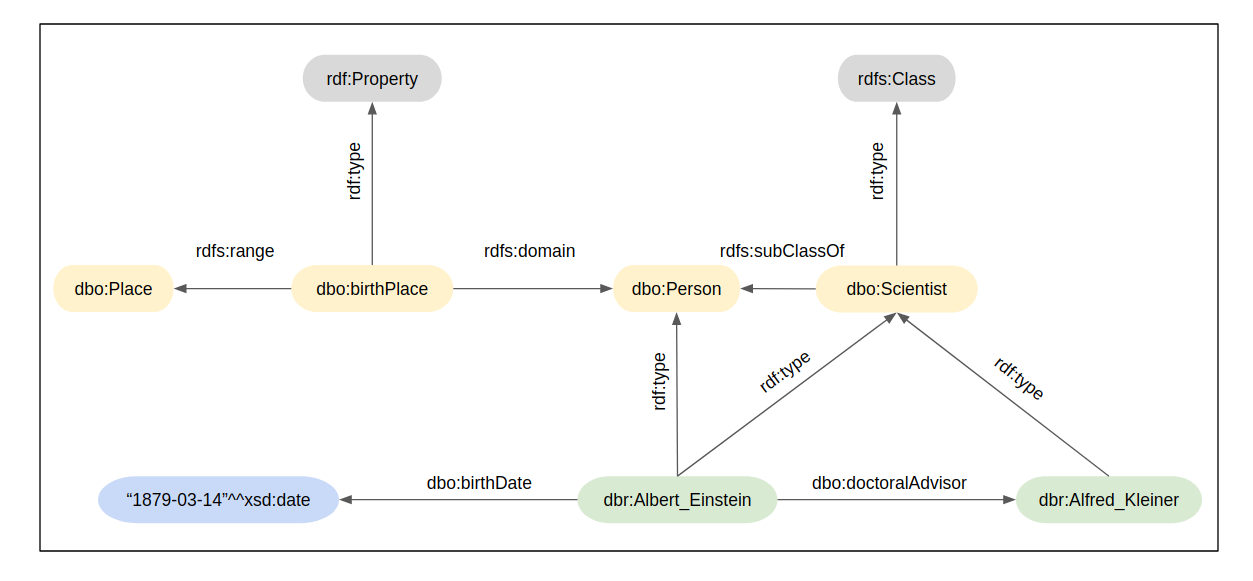
\includegraphics[width=\linewidth]{Figures/sec_KGs_RDF_graph.png}
 \caption{Example of a simple RDF graph}
 \label{fig:rdf_simple_graph}
\end{figure*} 
Knowledge graphs have been utilized in many real world information systems which require to leverage a structured, diverse, large-scale collection of data~\cite{DBLP:journals/semweb/Paulheim17,hogan2020knowledge}, e.g., the Google Knowledge Graph plays a very important role for enhancing the search engine results.  Besides the industry, knowledge graphs have been extensively utilized in various research areas (e.g., artificial intelligence) in academia. Moreover, the idea of leveraging structured knowledge, i.e., machine understandable knowledge by intelligent systems has been a goal of artificial intelligence research for decades~\cite{DBLP:journals/semweb/Paulheim17}. %Knowledge Graphs employ a graph-based form to represent knowledge, which can be domain specific such as facts about chemical interactions or domain independent. 

Furthermore, in \textit{Semantic Web} community the term knowledge graph is also used to refer to Semantic Web Knowledge Bases such as DBpedia, Wikidata, YAGO, etc.~\cite{DBLP:journals/semweb/Paulheim17} To facilitate the discussion, first we give the description of Semantic Web which was proposed by Tim Berners-Lee et al. as ``\textit{A new form of web content that is meaningful to computers}'', in 2001. Since then the fundamentals of the Semantic Web have been based on the idea of representing knowledge in a structured and machine understandable way. Today, knowledge bases are one of the most essential components of the Semantic Web.
They employ a graph-based form to represent knowledge, which can be domain specific such as facts about chemical interactions or domain independent. The facts in knowledge bases are modeled by directed edge-labeled graphs as shown in Figure~\ref{fig:rdf_simple_graph}. Such graphs consist of set of nodes such as \textsf{dbr:Albert\_Einstein, dbo:Scientist} and directed-labeled edges between those nodes such as \textsf{rdf:type, rdfs:subClassOf}. 
\begin{minipage}{\textwidth}
\begin{lstlisting} [caption={RDF document in turtle serialization},label=listing_rdf_serialization]

@prefix rdf: <http://www.w3.org/1999/02/22-rdf-syntax-ns#> .
@prefix rdfs: <http://www.w3.org/2000/01/rdf-schema#> .
@prefix xsd: <http://www.w3.org/2001/XMLSchema#> .
@prefix dbo: <http://dbpedia.org/ontology/> .
@prefix dbr: <http://dbpedia.org/resource/> .

dbo:birthPlace	rdfs:range	dbo:Place .
dbo:birthPlace	rdfs:domain	dbo:Person .
dbo:birthPlace	rdf:type	rdf:Property .

dbo:Scientist	rdf:type	rdfs:Class .
dbo:Scientist	rdf:subClassOf	dbo:Person .

dbr:Albert_Einstein	dbo:birthDate	"1879-03-14"^^xsd:date .
dbr:Albert_Einstein	rdf:type	dbo:Person .
dbr:Albert_Einstein	rdf:type	dbo:Scientist .
dbr:Albert_Einstein	dbo:doctoralAdvisor	dbr:Alfred_Kleiner .
\end{lstlisting}
\end{minipage}\\\\


Semantic Web knowledge bases follow standardized data modeling formats which facilitate the knowledge exchange. These standards include but not limited to \textit{Resource Description Framework} (RDF),  \textit{Resource Description Framework Schema} (RDFS) which is an extension of the RDF and \textit{Web Ontology Language} (OWL). The specifications of the data modelling formats are published by World Wide Web Consortium\footnote{https://www.w3.org/standards/} (W3C) that is the main international standards organization for the World Wide Web.%The Semantic Web knowledge bases follow  a standardized data model so called \textit{Resource Description Framework} (RDF) which is a formal language for describing structured knowledge. The  specifications of RDF  

The RDF standards allow to define different types of nodes in a knowledge base namely, \textit{resources} (entities on the Web) which could be anything like people, location, documents, etc., \textit{literals} that allow representing data type values such as dates, integers, etc. and \textit{blank nodes}. %which are not assigned to any identifier. 
The RDF resources are identified by unique \textit{Internationalized Resource Identifiers} (IRIs)~\cite{DBLP:journals/rfc/rfc3987} that allow identification of entities on the Web. However, blank nodes are not assigned to any identifier and thus they do not carry any additional information within a knowledge base. Instead, blank nodes can only indicate an existence of a thing. The representation of knowledge in knowledge bases is based on the idea of making statements about the resources in the form of RDF triples (\texttt{subject,  predicate, object}), where the subject could be an entity or a blank node, whereas the object could be an entity or a blank node or a literal. Note that literals can only be in an object position. Some of the RDF triple examples from Figure~\ref{fig:rdf_simple_graph} are (dbr:Albert\_Einstein rdf:type dbo:Person) and (dbr:Alfred\_Kleiner rdf:type dbo:Scientist). Note that RDF's name space is \\http://www.w3.org/1999/02/22-rdf-syntax-ns\# and abbreviated by "rdf:". There exist several serialization syntaxes to convert RDF graphs into machine readable forms such as N-triples\footnote{https://www.w3.org/TR/n-triples/}, Turtle\footnote{https://www.w3.org/TR/turtle/}, etc. Listing~\ref{listing_rdf_serialization} is the turtle serialization of the RDF graph, which is depicted in Figure~\ref{fig:rdf_simple_graph}.  Listing~\ref{listing_rdf_serialization} shows that the RDF vocabulary has been used to define resources (e.g., \textsf{dbr:Albert\_Einstein rdf:type dbo:Scientist}) and predicates (e.g., \textsf{dbo:birthPlace rdf:type dbo:Property}).

%Further, the knowledge is represented by the ontologies and 
%Figure~\ref{fig:rdf_simple_graph} illustrates that RDF can only define, i.e., assign type information to resources. 

\par Another particular RDF vocabulary is RDFS~\cite{DBLP:books/crc/Hitzler2010} which enables the specification of schema knowledge. For example, the definition of domain and range of properties (e.g., (\textsf{dbo:birthPlace rdfs:domain dbo:Person}), (\textsf{dbo:birthPlace rdfs:range dbo:Place})) and hierarchical relationships, i.e, sub classes (e.g., \textsf{dbo:Scientist rdfs:subClassOf dbo:Person}), sub properties and more besides~\cite{DBLP:books/crc/Hitzler2010}. Due to capability of specifying such schema knowledge, RDFS can also be referred as an \textit{ontology language}. Let us first discuss the term \textit{ontology}. According to \cite{gruber1993translation} ontology can be defined as follows:
\begin{definition}{(Ontology):\\}
\textit{"An ontology is an explicit, formal specification of a shared conceptualization. The term is borrowed from philosophy, where an Ontology is a systematic account of existence. For AI systems, what ‘exists’ is that which can be represented."}
\end{definition}
In this definition, \textit{conceptualization} implies that existing of an abstract model of a certain domain which contains identified relevant concepts and their relations. \textit{Explicit} denotes that meaning of all concepts must be defined and explicit. \textit{Shared} stands for consensus about the ontology and \textit{formal} refers to machine understandability.  

%Further it also defines the domain and range of properties. subclasses, subproperties, domains, and ranges amongst the classes and properties used in an RDF graph. 

%Note that each RDFS document is also an RDF document.
Figure~\ref{fig:rdf_simple_graph} illustrates that the simple ontologies can be modeled by RDF(S), however, for modeling more complex representation of knowledge the Web Ontology Language (OWL) is being used. OWL is based on formal logic and supports much greater expressiveness than RDF(S). Further, it allows logical reasoning on the knowledge and thus enables to deduce implicit knowledge which is not explicitly modeled. More details about OWL can be found  in~\cite{DBLP:books/crc/Hitzler2010}.
% \begin{figure*}[t]
%  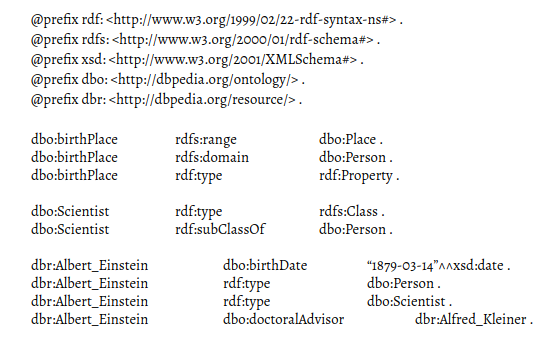
\includegraphics[width=\linewidth]{Figures/sec_KGs_RDF_turtle_serialization.png}
%  \caption{RDF document in turtle serialization}
%  \label{fig:architecture}
% \end{figure*}
\subsection{Open Knowledge Graphs} \todo{check "on the other hand"}
Open knowledge graphs are openly available and freely usable. There are different ways of constructing open knowledge graphs, i.e, they can be curated by a small group of people or crowd sourced by a large group of people or created by utilizing automatic or semi-automatic methods~\cite{DBLP:journals/semweb/Paulheim17}. In the following we give the example of knowledge bases which have been built by different methods:
\begin{itemize}
\item \textbf{Cyc and OpenCyc~\cite{DBLP:journals/cacm/Lenat95}.} Cyc is one of the oldest curated knowledge bases of common sense which is developed and maintained by the CyCorp company starting in 1984. The artificial intelligent project Cyc, represents millions of common sense facts. For example:
\begin{itemize}
\item"You have to be awake to eat.", 
\item"You cannot remember events that have not happened yet.".
\end{itemize}
Cyc aims to be served as a structured data source especially to the artificial intelligence based applications such as information retrieval, speech recognition, etc.~\cite{DBLP:journals/cacm/Lenat95}
%The domain of CYc is all of human consensus reality, such as thecommon sense  
Since Cyc is proprietary, a small version of it so called OpenCyc has been made publicly available. Further, there used to be an existing Semantic Web endpoint to OpenCyc%\todo{tell that you are reporting the numbers from a published paper}
, which also contains links to other Linked Open Data\footnote{https://lod-cloud.net/} datasets such as DBpedia. The 2012 version of OpenCyc contains approximately 120,000 instances and 2.5 million facts defined for those instances; its schema consist of approximately 45,000 type hierarchy, and 19,000 possible relations~\cite{DBLP:journals/semweb/Paulheim17}. The CyCorp company, the developer of OpenCyc, has stopped online support for its knowledge base since March 2017.\\

\item \textbf{WordNet~\cite{fellbaum98wordnet}.} WordNet is a large lexical knowledge base for English language created in the Cognitive Science Laboratory of Princeton University staring in 1985. WordNet includes the lexical categories of different types of words, i.e., nouns, verbs, adjectives and adverbs. The words that are from the same lexical category grouped into unordered sets of cognitive synonyms, called \textit{synsets}. Synsets are interlinked by the means of semantic links such as hyperonymy, meronymy. This knowledge graph can be navigated easily with the browser. WordNet is publicly available and can be downloaded freely. The 3.0 version of WordNet contains in total 117,659 synsets for 155,287 unique strings,including 82,115 synsets for 117,798 nouns, 13,767 synsets for 11,529 verbs, 18,156 synsets for 21,479 adjectives, 3,621 synsets for 4,481 adverbs, as well as 206,941 word-sense pairs,including 146,312 for nouns, 25,047 for verbs, 30,002 for adjectives, 5,580 for adverbs.\\

\item \textbf{Freebase~\cite{DBLP:conf/sigmod/BollackerEPST08}.} Freebase is a public knowledge base which is created through crowd sourcing by the announcement of American software company Metaweb in March 2007. In contrast to other curated knowledge bases, e.g., Cyc, which required more than 900 person years to create~\cite{DBLP:journals/semweb/Paulheim17}, Freebase provided an interface to the public editors.  Thereby, the editors could directly contribute to the knowledge base by editing structured data with schema templates. Besides the contribution of the editors, Freebase integrated knowledge  from Wikipedia~\cite{farber2015comparative}. In 2010, Freebase acquired by Google and on August 31, 2016, it was completely shut down. The last version of Free-base contains roughly 50 million entities and 3 billion facts. The Freebase schema comprises roughly 27,000 entity types and 38,000 relations~\cite{DBLP:journals/semweb/Paulheim17}.\\

\item \textbf{Wikidata~\cite{DBLP:journals/cacm/VrandecicK14}.} Wikidata is a collaboratively edited knowledge base with community effort and it is operated by the Wikimedia foundation. Wikidata has been extensively exploited as a main data source in wide range of information systems, especially in the Semantic Web community. Unlike aforementioned KBs Wikidata does not only contain facts but also source of the facts so that the validity of facts can be approved. Moreover, after the shut down of Freebase, its data moved to Wikidata. To date, Wikidata contains roughly 83,343,004 instances\footnote{https://www.wikidata.org/wiki/Wikidata:Main_Page} and 1,036,340,466 million statements\footnote{http://tools.wmflabs.org/wikidata-todo/stats.php}. Its schema defines roughly 7,450 relations\footnote{https://www.wikidata.org/w/index.php?title=Special:ListProperties}.\\

\item \textbf{DBpedia~\cite{DBLP:conf/semweb/AuerBKLCI07}.} DBpedia is the most popular KG in LOD cloud which was initiated by the researchers from the Free University of Berlin and the University of Leipzig, in collaboration with OpenLink Software~\cite{farber2015comparative}. Unlike aforementioned KBs, DBpedia has been created by automatically extracting structured and multilingual knowledge from Wikipedia, i.e., Wikipeida infoboxes. The types of infoboxes in Wikipedia are mapped to the DBpedia ontology, further the attributes of these info boxes are corresponds to the properties in DBpedia ontology~\cite{DBLP:journals/semweb/Paulheim17}. Similar to Wikidata, DBpedia has been extensively utilized in various research fileds of Semantic Web. The most recent version of the main DBpedia (i.e., DBpedia 2016-10, extracted from the English Wikipedia based on dumps from October 2016) contains 6.6M entities\footnote{https://wiki.dbpedia.org/develop/datasets/dbpedia-version-2016-10}, 13 billion facts (RDF triples), and the schema comprises 760 classes, 1,105 object properties, 1,622 datatype properties.\\

\item \textbf{YAGO~\cite{suchanek2007yago}.} Like DBpedia, YAGO is also extracted from Wikipedia and developed at the Max Planck Institute for Computer Science in Saarbrücken since 2007~\cite{farber2015comparative}. In contrast to DBpedia, YAGO comprises information not only from Wikipedia (e.g., categories, redirects, infoboxes) but also WordNet (e.g., synsets, hyponymy), GeoNames~\cite{farber2015comparative,fabian2007yago}. Further, DBpedia creates different interlinked KBs for each Wikipedia language edition (e.g., English, German, etc.), however, YAGO aims to build fusion of knowledge which extracted from various Wikipedia language editions. The latest release of YAGO, i.e., YAGO3, contains approximately 4.5 million entities and 24 million facts about such  entities  in  10  languages.   The  schema  comprises  488,496  classes  and  77 manually defined relations~\cite{DBLP:conf/cidr/MahdisoltaniBS15}.\\
 
\item \textbf{NELL~\cite{DBLP:conf/wsdm/CarlsonBWHM10}.} Never Ending Language Learning\footnote{http://rtw.ml.cmu.edu/rtw/} (NELL) is a project developed by a research team at Carnegie Mellon University since January 2010. Unlike DBpedia and YAGO which utilizes semi-structured content (e.g, Wikipedia Infoboxes)  as a base, NELL designed to exploit unstructured data to extract meaningful knowledge. In other words, the project attempts to conduct two main tasks everyday.
First, it attempts to extract facts from text found in in hundreds of millions of web pages (e.g., servedWith(tea, biscuits)).
Second, it attempts to improve its fact extracting capability, so that next time it can extract more facts from the web, more accurately. Each extracted fact has a weight which reflect the confidence of it. The system is still running today and has been extending its knowledge base by since the project has developed. So far, NELL has accumulated over 50 million candidate beliefs by reading the web and 2,810,379 of these beliefs are in high confidence. On NELL website, only the beliefs that has the high confidence are displayed. 
\end{itemize}\vspace{0.5cm}
\noindent Most of the open knowledge bases contain links to other RDF data sources. By doing so, users can navigate between
different data sources by following RDF links. Hence, the Semantic Web aims to make meaningful links between publicly available RDF data sources (e.g, DBpedia, Wikidata, etc.) to enable persons and machines to explore \textit{Linked Open Data}~\cite{} freely. In the following let us  briefly discuss the phrase \textit{Linked Open Data}.\\

\subsection{Linked Open Data}
%\noindent \textbf{Linked Open Data (LOD).}
Linked Open Data (LOD) refers to publicly available RDF data which is identified via URI and accessible via HTTP on the Web. Further, those RDF datasets are linked to other datasets via URI. Accordingly, the Linked Open Data project aims to identify datasets that are available under open licenses, re-publish
these in RDF on the Web and interlink them with each other~\cite{DBLP:conf/www/BizerHIB08}. \\
The principles of Linked Data were first outlined by Berners-Lee in 2006:
\begin{itemize}
\item Use URIs as names for things.
\item Use HTTP URIs so that people can look up those names.
\item When someone looks up a URI, provide useful information, using the standards (e.g. RDF).
\item Include links to other URIs, so that they can discover more
things.
\end{itemize}
The four rules provide broad guidance on which publishing RDF data can be based. LOD is accessed using traditional HTML
browsers and users can easily explore and navigate between different data source.

The network of publicly available RDF datasets that are in concordance with linked data principles has grown globally. As of April 2017, the number of the publicly available RDF datasets is 9960 which contain roughly more than 149 billion facts and roughly more than 800 million links.\todo{check the numbers} The visualization of interlinked RDF datasets which is refered as \textit{Linked Open Data Cloud\footnote{https://lod-cloud.net/}} has been  created by~\cite{LOD_cloud}.  Figure ~\ref{fig:lod_cloud} illustrates the evolution of the LOD cloud from its beginning in 2007 until 2019.  

Each node in the networks represents one dataset. As of March 2019, the huge network contains 1,239 datasets with 16,147 links. DBpedia has been one of the most popular datasets in these networks across the years. 
%Semantic web is about making meaningful links between heterogeneous data sources to enable persons and machines to explore a "web of data" 
\newpage
\begin{figure}[t]
%\centering
\captionsetup{justification=centering, margin={0cm,0.5cm}}
\begin{minipage}{.5\textwidth}
  \centering
  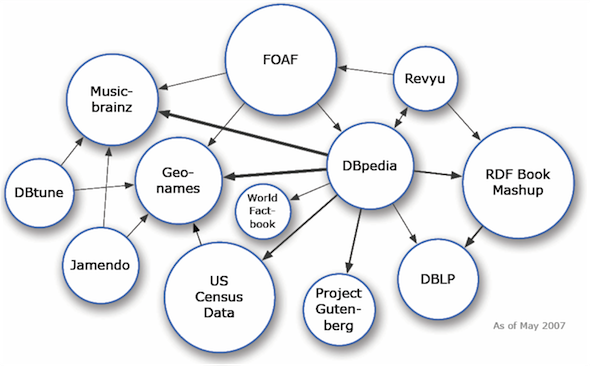
\includegraphics[width=\linewidth]{Figures/LOD/lod-cloud_2007.png}
  \caption*{March 2007 (12 datasets)}
  \label{fig:test1}
\end{minipage}%
\hspace{0.5cm}
\begin{minipage}{.5\textwidth}
  %\centering
  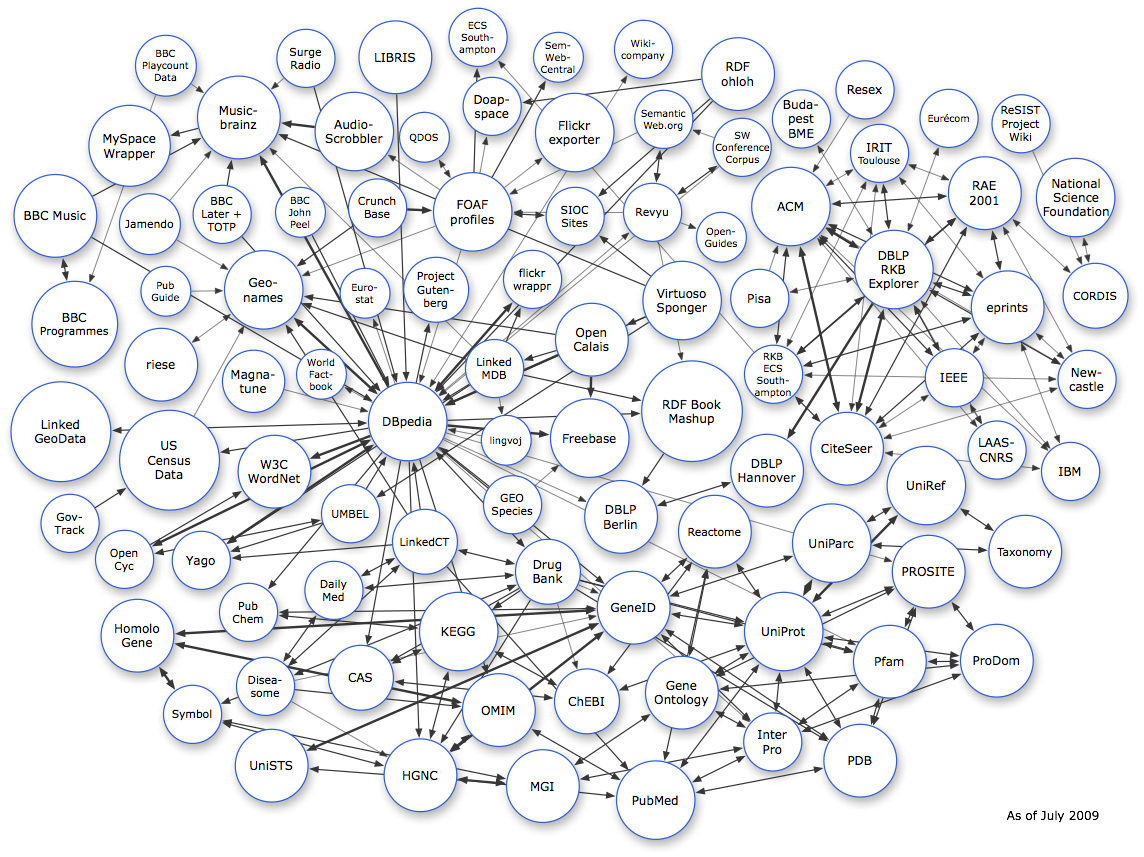
\includegraphics[width=\linewidth]{Figures/LOD/lod-cloud_2009.png}
  \caption*{July 2009 (95 datasets)}
  \label{fig:test2}
\end{minipage}
\end{figure}
\vspace{5cm}

\vspace{10cm}
\vspace{5cm}
\begin{figure}
\centering
\captionsetup{justification=centering, margin={0cm,0.5cm}}
\begin{minipage}{.5\textwidth}
  \centering
  \includegraphics[width=\linewidth]{Figures/LOD/lod-cloud_2014.png}
  \caption*{March 2007 (12 datasets)}
  \label{fig:test1}
\end{minipage}%
\begin{minipage}{.5\textwidth}
  \centering
  \includegraphics[width=\linewidth]{Figures/LOD/lod-cloud_2017.png}
  \caption*{July 2009 (95 datasets)}
  \label{fig:test2}
\end{minipage}
\end{figure}


%\input{Figures/fig_deneme}
\clearpage

\begin{figure}[t!]
\centering
 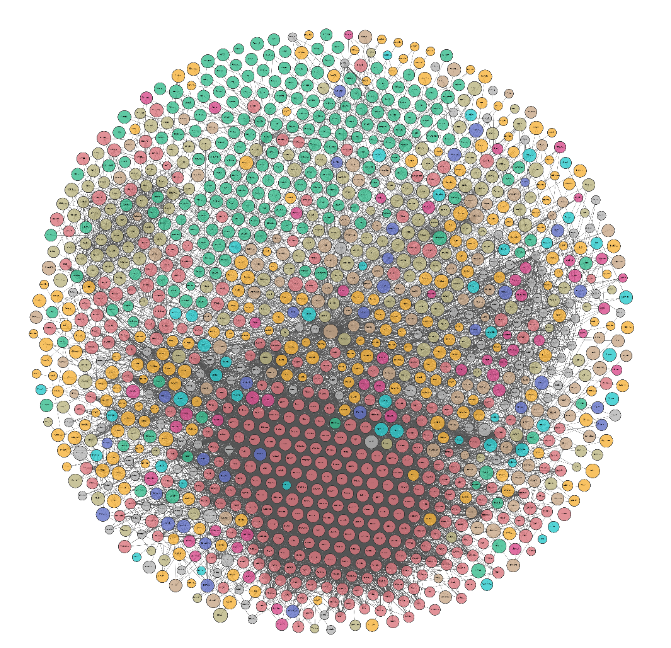
\includegraphics[height=9cm,width=9cm]{Figures/LOD/fig_LOD_2019_clean.png}
 \caption{March 2019 (1,239 datasets)}
 \label{fig:lod_cloud}
\end{figure}


%\clearpage

\section{Semantic Similarity}  \label{cha:semantic_similarity}
%HANDBOOK OF NATURAL LANGUAGE PROCESSING
\section{Summary}  
\label{cha:foundations_basics_summary}



\chapter{Text Categorization}
\label{cha:foundations_text_cat}

%classification

%Basic text classification schema explain each step
%Characteristic of Text
%\subsection{Text Categorization}
%Short, long text categorization...
\section*{}
The World Wide Web also known as Web has become one of the largest global collection of information %interconncete knowledge 
with over 1.5 billion websites\footnote{https://www.internetlivestats.com/total-number-of-websites}. The Web is a global network environment where documents and other Web sources are identified by Uniform Resource Locators (URLs)~\cite{berners1998uri}. The documents are interlinked by hyper links~\cite{jacobs2004architecture} and accessible over the Internet. This global document repository encompasses almost every topic of human interest. The usefulness of Web document access can be seen from the fact that Google processes over 40,000 search queries every second on average, which translates to over 3.5 billion searches per day and 1.2 trillion searches per year worldwide\footnote{https://www.internetlivestats.com/google-search-statistics/}. 

Furthermore, today, billions  of  users$^1$ access and even contribute to this massive information exchange platform. Due to the large number of contributions as well as the digitization of all areas the content of the Web is drastically multiplying~\cite{STCImprovedby}. %Thus, there arouses a necessity of automatic analyzing and processing techniques of such data in order to satisfy a particular need of information~\cite{STTopicMemory}.
As a result, the fields of Natural  Language  Processing (NLP)~\cite{Jurafsky:2009:SLP:1214993} evolves in parallel, which concern the automatic analyzing and processing of natural language documents in order to satisfy a particular need of information. In other words, NLP is a field of computer science, artificial intelligence, and computational linguistics whose techniques are specifically designed to extract meaningful information from natural language documents. Some examples of NLP applications are Spelling and Grammar Checking, Auto  completion, Text Categorization, Text Summarization, Information Retrieval, etc.   Among those applications, text classification is the fundamental one which has been proven to be useful in various applications, such as sentiment analysis, news feed filtering and categorization, etc.~\cite{STTopicMemory}.

%Importance necessity of classification Application
Text categorization (a.k.a text classification) aims to assign one or more predefined classes or categories to natural language documents based on the attributes of the each text document. The textual data can be anything ranging from a phrase, sentences, paragraphs or an entire document. %Due to recent advancement of NLP many researchers are now concerned with developing new applications by exploiting text classification methods Some examples of text classification... 
However, with the rapid growth of online platforms such as Facebook, Twitter, online forums, etc. the Web users are now generating more and more \textit{short text} data. A large body of daily generated content of the Web, such as short text messages,micro blog posts, search queries etc. have become an important form for individuals to share information~\cite{STTopicMemory}. The main characteristic of short text is that the length of the text is very limited which is no longer than 200 characters~\cite{song2014short}. Further, unlike other documents short texts are usually rather ambiguous and sparse. Due to the limited length of the text which is only several to a dozen words~\cite{song2014short} the ambiguity cannot be resolved by depending on the context. Further, since the context is rather limited feature extraction is rather difficult. Such characteristics pose several major challenges to short text categorization tasks. While conventional text classification methods such as Support Vector Machines (SVMs) have demonstrated their success in classifying long and well structured text, as e.g., news articles, in case of short text they seem to have a substandard performance~\cite{STTopicMemory}.


\par Recently, several deep learning approaches have been proposed for short text classification, which demonstrated remarkable performance in this task~\cite{sentiment/aaai/MaPC18,DBLP:conf/emnlp/ChenSBY17}. The two main advantages of these models for the classification task are that minimum effort is required for feature engineering and their classification performance is better in comparison to traditional text classification approaches~\cite{WeaklySupervised}. However, the requirement of large amounts of labeled data remains the main bottleneck for neural network based approaches~\cite{WeaklySupervised}. Acquiring labeled data for the classification task is costly and time-consuming. Especially, if the data to be labeled is of a specific domain then only a limited number of domain experts is able to label them correctly, which makes it a labor intensive task.

In this thesis, we are concerned with
 %For instance, Google processes over 40,000 search queries every second on average which translates to over 3.5 billion searches per day. Maybe also news feed info
\begin{comment}
\section{Text Categorization}

\label{cha:foundations_basics_text_cat}
The problem of \textit{categorization} has been extensively studied in various domains i.e., data mining, machine learning, database, and information retrieval communities with wide range of applications such as document categorization, spam filtering, medical diagnosis~\cite{book_survey_text_class_algorithms}. The main goal of a categorization task is to assign or more class labels to data instance for which the class is unknown. The general categorization task assumes each class label is a predefined categorical value, e.g., \textit{Sports}, \textit{Science}, \textit{Politics}, etc. The problem of text categorization is closely related to such type of a task. In other words, text categorization aims to assign one or more predefined classes or categories to natural language documents based on the attributes of the each text document. It is one of the most fundamental tasks in Natural Language Processing with wide applications such as sentiment analysis, ... %Text categorization finds its applications in variouse domains such as ...
Text classification
has a wide variety of application scenarios, for instance: \newline% explain here the applications
%TODO enumaration here and the KBs
%Short Text Classification: A Survey yo can have a look at it

\textbf{Information retrieval.}
Information retrieval systems and search engines have extensively made use of text categorization techniques~\cite{survey}. The IR task can be formulated as a given user query the task is to retrieve all the relevant documents to the query while retrieving as less relavent documents as possible. It is a crucial task in variaty of domains as it helps to find a quickly finding relavent information within massive natural language text documents which are most of the time highly unstructured. 


\textbf{Document organization.}
A variety of text categorization techniques can be exploited to for document organization in many domains. These include large collection of patent documents, Web content, digital libraries, academic articles. In addition, many companies nowadays required to organize and analyse business information like legal documents, emails, web pages, etc. 

\textbf{Sentiment analysis.}
One of the most common text categorization problems is sentiment analysis. It aims to extract subjective information such as positive or negative or neutral from text documents. For example, it can help business to understand the social sentiment of their brand and adopt the product accordingly.  

\textbf{Spam filtering.}
It is often desirable to determine the spam emails i.e., unwanted, and/or virus-infested emails in order to avoid it from getting into email inboxes. Most of the business email networks use spam filtering systems to protect the system from the many possible risks. The goal of the spam filtering systems is to decide whether a given email spam or not. To this end, binary text categorizations techniques have been extensively utilized.

There exist three main types of text categorization methods types of systems, namely, \textit{manual}, \textit{Rule-based}, \textit{Machine Learning based}. Although often manually labeled documents by human highly accurate, it is the most expensive one among the aforementioned methods. Especially, if the text to be labeled is of a specific domain only several domain experts can categorize such data.pretty slow and expensive. On the other hand, Rule-based systems leverage user defined linguistic rules to perform the categorization task.manually build and maintain
a rule-based system, These rules are designed to utilize the semantic content of the documents to assign relevant categories. Each rule consist of a pattern and the corresponding category~\cite{DBLP:conf/ijcnlp/ChakravarthyJRGB08}. In contrast to aforementioned systems, the machine learning based systems rely on the past observations to make a prediction. In other words, such systems can learn the associations between the content of the documents and the labels by utilizing available training data (pre-labeled). Altough machine learning based systems seem to be the most common, they require large amount of labeled data. Further, not only the size of the data is an issue but also the characteristic of the data is also important to build an successful machine learning based system.  


%semi-supervised and weakly supervised Supervised is too expensive % explain each method in 1 or 2 sentences
In this thesis we focus on where the labeled data is not available

\textcolor{red}{Figure text classification fi from Short Text Classification: A Survey}

An overview of tasks involved in text categorization is shown in Fig In the following sections %explain each step in 1-3 sentence

%classification

%Basic text classification schema explain each step
%Characteristic of Text
%\subsection{Text Categorization}
%Short, long text categorization...
\end{comment}

\section{Short Text Categorization}
%Short Text Classification: A Survey
%Short Text Understanding Through Lexical-Semantic Analysis
%Combining Knowledge with Deep Convolutional Neural Networks for Short Text Classification
%Example is necessary
The main characteristic of short text is the length of text is very limited which is no longer than 200 characters than~\cite{song2014short}. In other words, unlike normal documents short text consist of from a dozen words to a few sentences~\cite{song2014short}. Due to grow of Web e-commerce and online communica produced such as Web search snippets, forum and chat messages
For example mobile text
tweet length
Due to the availability  successfully categorizing them becomes increasingly important in wide range applications such as ...

Besides its limited length, short texts have other uniqe characteristic 
Sparseness:\\
Immediacy:\\
Non-standardability:\\
Noises and imbalanced distribution:\\
Ambiguity:\\
In the following given example 

%explain short text categorization task
On the other hand, short text categorization similar to arbitrary text categorization (see Sec ) aims to...
Following we give the formal definition of short text categorization task 

Due to the aforementioned main characteristic of short text conventional text categorization models which rely on \textit{weighted word} (see Sec ) cannot perform well. Therefore, designing successful short text categorization system requires additional effort. Unlike arbitrary text categorization systems, short text categorization systems adopt more sophisticated text representation methods. In other words, should be able to capture more semantic and syntactic information from the text. In the related work section we review the state of the art short text categorization approaches which adopt various methods for short text representation. 
\subsection{Related Work}
\section{Text Preprocessing}
%Text Classification Algorithms: A Survey
%HANDBOOK OF NATURAL LANGUAGE PROCESSING
%Text Analytics with Python
%any NLP system,
Most of the time, text data in its raw form is not well structured and contains unnecessary words which do not add any value to the categorization performance. In fact unnecessary words can have adverse effects on system performance. Therefore, for the successful text categorization system the first step is preprocessing which is crucial for many applications. Following we briefly explain the most common text preprocessing techniques:

Text Tokenization: Given a sequence of text text tokenization methods breaks the text into smaller parts called tokens. Often, there are two types of  tokenition systems aims to split the text into sentences or words. Following we give the example of sentence and word tokenization\\

\textbf{Noise removal:} Depending on the type, documents could contain unnecessary special characters like hashtags. Such characters might have negative impact on the categorization performance. Therefore, many NLP applications remove punctuation
and special characters from texts.\\

\textbf{Case conversions:}\\
Text documents might contain inconsistent capitilazation of words. This is can be critical a problem especially for the text categorization systems. For example refer to the same thing. Therefore, it would be inappropriate to regard them as two different words in text analysis. In such case converting all the words to lower case can help to achive consistency in terms of capitalization form of the words. On the other hand this procesess can be problematic for interpretation of some words like (e.g., “US” (United States of America) to “us” (pronoun))~\cite{text_class_survey_2019}. Moreover for different languages such as German it might be even better to retain the capitalization form of the words. Overall, based on the characteristic of a corpus e.g., language the case conversition can be applied.  

\textbf{Removing stop-words:} Depending on the length, text documents include many stop words which do not do not contain important significance. Therefore, many NLP applications remove the stop words before start processing the text data. Stop words are the like common words of a language such as ... which do not add any information to the document that can help to perform better text categorization. Further, another benefit of removing stop words is it helps to reduce the size of the dataset which is critical when dealing with the large scale corpus.

\textbf{Stemming and Lemmatizing:} Text documents could contain different form of same words such as .. Stemming and lemmatizing techniques aim to reduce morphological variation of words. While stemming tries to reduces the inflected words into their base form lemmatizing tries to bring words down to word's lemma form, i.e., dictionary form. Although stemming and lemmatization seem to be closely related there is a main difference. In contrast to lemmatization which aims to correctly identifiying meaning of a word based on its context, stemmer operates on asingle word without considering its context. Further in comparison to lemmatizations stemmers are much easier to implement and they are faster. 

For stemming we give the following example:\\

On the other hand for lemmatization we give the following example:\\

%\subsection{State of the Art}
\section{Feature Extraction and Selection}
%Machine Learning for Text sec 5.2
%Text Classification Algorithms: A Survey
%Weighted Words (BoW, TFIDF)
%Word Embedding at least mention and explain other section


%Lexical Representations,%Syntactic Representations,%Semantic Representations\\
\section{Text Categorization Algorithms}
%Machine Learning for Text
\textbf{Decision Trees and Random Forest:}\\
A Decision tree decomposition of data hychacally in which the division is achieved by numerous decision i.e., conditions on the attributes~\cite{book}. The main goal is to split the data into attribute regions which each represents a class label. Random forests are known to be highly robust and accurate implementation of decision trees. \\
\textbf{Decision Tree Construction:}\\
Decision trees partition the data space tree-like in a top down fashion. Each leaf corresponds to a class label and each predicate of the tree represents a split condition which is similar to feature selection creteria in categorization. Often, in text categorization each split criteria corresponds to frequency of one or more words present in given texts or a presence of absence of a word. The split criteria can use single wheares the one uses multiple attributes called \textit{multivariate split}.
Given a text document starting from root splits are recursively applied and in order to identify the branch to followed in a top down fashion until the relavent leaf node is reached. 

This way of creating a tree could cause \textit{over fitting}. Because even with the randomly labeled training data this way of creating tree will provide 100\% accuracy on the training set. This type of a tree will cause inaccurate predictions on the test set because one cannot expect to learn anything from such training data. As a result the performance of a tree will poor even the characteristic of the test data highly suitable for a cateforizazion task. This problem is tackled by \textit{pruning} of the lower level of the tree therefore, the leafes of the tree may contain multiple class labels. reades detail cite
\textbf{Splitting a Node:}
As an example in the folowing conditional entropy is used as feature selection criteria in which  only the presence or absence of a term in a document is used as the split criterion

Note that The split criteria can use any of the ...

For the given example, the split is tested for each term tj, and the one providing the lowest conditional entropy is selected. The

Once the tree is built, the categorization of a test sample is straightforward. In other words, for each test sample starting from root based ont he split criteria which branch to follow is determined. This proceses repeated in a top-down fashion until eht leaf node is reached.

\textbf{Multivariate Splits:}
In the case Multivariate Splits each split createria has multiple appributes and the distributed(?) representation of docments are used to implement multivariate Splits. Sample \textit{r} (user defined parameter) directions such that Y1 ...Yr
in the d-dimensional vector space and
project all the documents in L along each of these r directions. .... later 

\textbf{Random Forests:}


\textbf{Naive Bayes Classifiers}\\
The naive Bayes classifier is a probabilistic model which is based on a bayes theorem. To facilate the discussin we give the definiation of Bayes theorem as follows:


Naïve Bayes algorithm has been studied extensively  and it is still the one of the standard baseline for text categorization models. The model is a probabilistic generative model which assumes that the given text corpus is generated from a mixture of different classes. The generative process is defines as follows~\cite{aggarwal2018machine}:

1.\\
2.

The outcome of this generative process assumed to be training and test data. Generally, training data is utilized to approximate the parameters of the probabilistic model. Subsequently, the model then is used to estimate the probability of generation of test document from each class. Finally, the each test sample would be labeled with the class which has the highest probability. for naive bayes classification two classed of models, namely, Multivariate Bernoulli Model, Multinomial Model: are being used commonly.

\textbf{The Bernoulli Model}
The presence or absence of each term in the document is being used to model Bernoulli model. The vector representation of documents are sparse binary vectors where the frequency of each term is ignored. Bernoulli probabiities are


The naive bayes model assumes that presence or absence of the various terms are conditionally independent with respect to the given class. This is the main reason why the term \textit{naive} is used to refer this model. Because in real world setting often this assumption is not correct. 
In the training phase the model estimates the maximum likelihood values of the the parameters p(r)
j and r using only the training data. On the other hand, in the testing phase those parameters are utilized to predict the label of a given test document. 

\textbf{Multinomial Model:}\\
\textbf{Nearest Neighbor Classifiers:}\\
The main idea of the model is given a test instance identify the k-nearst neighbours of this point. Then compute number of neighbours that belong to each class. Finally, the class with the largest number of points is returned as a relavent to the given test sample. A straightforward implementation of the nearest-neighbor method requires no training phase yet it requires requires O(n) similarity computation in order to find the k nearest neighbours for each given test instance. However, this complexity problem can be addresed by  utilizing a data structure called an inverted index~\cite{}.

k is a parameter, depending on the training set it is value can be determined. In other words, different values of k can be tried on training sent and the one at which the highest accuracy is achieved on the training data is used. Further, in order the find the optimal value of k the validation set is exploited in a leave-one-out manner.
 
A special case of k nnn algorithm is when the value of k is set to 1. Such a model is lack of robustness i.e., can overfit depending on the training data at hand. However, if the size of the training data sufficiently large then then it can achieve an error anywhere close the Bayes error rate. There are also other ways of avoiding the error that may cause by k set to 1 e.g., weighted nearest neighbors, or adaptive nearest- neighbor classification.  random forests and kernel support vector machines, can be shown to be adaptive nearest-neighbor classifier. In the next sections we explain them. 

\textbf{Weighted Nearest Neighbors:}\\
k-nn performs the cartegorization by relying on the similarity between the instences. In addtion, it can be viewed as a similarity weighted classifier which helps the generlization of it to models like random forests and kernel support vector machines.
%formula:

the similarity value can be considered as weight. Different similarity measures can be utilized e.g., cosine similarity. In the case of cossine simila  seting  K(Z,Xi) to the dot product Z · Xi. Gaussian kernel similarity is alternative similarity measure as:
%formula 5.25

where equals to bandwith. The value of σ can be deermined by using a leave-one-out validation approach.
\\

\\
\textbf{Rule-Based Classifiers:}\\
Rule based classifiers define set of \textit{"if then"} rules where left and right hand sides of it refered as \textit{antecedent}, consequent, respectively. An example form of a rule as follows:\\
\\

The left hand side of the rule, i.e, antecedent contains set of conditions as  

where t is a term and X is a document and each condition refered as conjunct. In such senario a classificatoion performed based on the presence or absence of a words oin documents. If a certain word presents in the document then the rule is triggered or fired, i.e., the condition is satified by the given instance. Once the rule is fired then the class label is generated. Moreover, a rule can be in a form of Qi c where ...

Rule based classifiers similar to other machine learning based classifiers like have training and testing phase. In the training phase based on the training set the set of rules are generated and in the test phase the rules are discovered that are triggered by the given each test instance. In the subsquent sections we briefly introduce some rule generain algorithms.\\

\textbf{Sequential Covering Algorithms:}
The Sequential Covering Algorithms generates rules for each class individually, i.e., at one time based on  Learn-One-Rule procedure. In other words, by treating the class of interest as the positive class and the rest of the classes are the negative the rules are generated iteratively for the positive class. This procedure continues iteratively untill the predetermined error thereshold rate reached. Once the rules are generarted for the positive all the training samples that are covered by the positive class removed from the training set. This procedure continues until the rules are generated for each class.

\textbf{Learn-One-Rule:}\\
In this section we explain the lor procedure by for class c. The basic idea in lor considering only presence of terms as a criteria. Because considering 
absence of terms in documents can cause over-fitting. 
Further, each term which is assoited with the class c then added to the antecedent one by one. The approach start with empty rule. There are several criterion that can be taken into account for including a term to the rule such as accuracy, FOIL’s information gain, likelihood ratio, entropy, etc.
For the sake of simplicity, we will concisely denote a rule such as ...

1. One of the simplest criterions is accuracy based. In other words, given the positive class the terms are added to the antecedent that increases the accuracy. In order to avoid overfitting the accuracy of adding a term to the antecedent defined as follows:
%formula 5.37

2. First Order Inductive Learner FOIL’s information gain is can be an alternative criterion of adding a term to the antecedent
%formula 5.38

The main idea of this measure is to select the rules with the high coverage. 

Note that terms can be included in the rules until the 100\% accuracy achieved on the training set. However, this is absolutely causes an overfitting. Therefore, another approach has to be taken. similar to decison trees antecedent pruning is necessary.\\
%Rule Pruning

\textbf{Generating Rules from Decision Trees:}\\
As explained in sec , each attribute of a decision tree corresponds to a condition. Hence, each predicate in a decision tree can be considered as a rule. Then, for each path in a decision tree the conditions can be conjuncted until the leaf node is reached to generate the rules for the corresponding class. However, since decision trees can contain absence of attributes as a condition, therefore rules can also contain such condition. Finally, the rules are processed and pruned to improved the accuracy with the separate validation set. \\
\textbf{Associative Classifiers:}\\
The basic idea of Associative Classifiers rely on exploiting the association rule mining techniques.
The simple rule is of the form:

where S set of terms and the c is a class label. The set of terms in S, in the antecedent corresponds to the presence of all the terms in a document, only then the rule can be tireggered, i.e., the class label c can be returned. 
\textbf{Prediction:}
The prediction pahase is straightforward. For each test instance a class labeles are identified based on the fired rules. However, the clange occurs when the generated class labels are confilict with eachother. then the simpleset approch is using the use the sum of the confidences of all the fired rules for a particular class.

\textbf{Linear Classification and Regression} (SVM, Logistic Reg,)\\
\textbf{Support Vector Machines:}\\
The basic idea behind svms is to data points belong to 2 classes based on a margin. SVMs first creates two hyperplanes so called \textit{margin hyperplanes} symmetrically on each side of the decision boundary in a way that most points lie on either side of the hyperplanes. Figure shows. 
The decision surface W · X = 0 lies in the middle of the two hyperplanes and it is same distance, i.e., \textit{margin} where W · X =1 and W ·X = −1 . Note that the points that are lying between the margins are penalized and this region reflects the uncertainty points called bounded support vectors. Moreover, two hyperplanes could also touch one or more training data points as shown in Figure and such data points referred to as free support vectors.
The common variation of SVM objective function as follows:
%formula Dual optimization SVM

where...
C is chosen empirically, i.e.,  value that maximizes the accuracy. The points that violate the margin penalized by C and the represent the amount by slack variable. Therefore the main goal of the training function is to minimize  e each ξi. 


\\
\textbf{Logistic Reg:}\\
Logistic regression is a probabilistic model which predicts probabilities of classes instead of classes.
The objective function of lr is defined as follows:
%formula 6,29
And the prediction od a test instance can be performed in two different was as follows:
%Deterministic
%Probabilistic
Often, the probabilistic prediction is and  learned using stochastic gradient descent
stochastic gradient-descent iterations the gradient defined as follows:
%formula 6.30
%formula 6.31
Typically, lr assumes that the dependent variable y is generated from a Bernoulli probability distribution that defined by a function of the feature variables like 

Now the prediction function can be written more generally y
%formula 6.32
Depending on the target variable it is possible to use different type of distribution.
The likelihood of the entire training data set with n pairs of
%formula 6,33

\textbf{Multinomial Logistic Regression and Other Generalizations:}\\
As it has already mentioned before it is possible to generalize the lr model depending on the aplication at hand. Given a k-class problem the dependent variable y is generated as follows:

Then the classes have the probability distribution as:
%formula 6.34
The loss function then is
%formula 6.35
refered ass cross entropy

Finally, the stochastic gradient- descent steps can be used to update the parameter

%\subsection{State of the Art}
\section{Evaluation Methods}
%Dataless, Supervised, weakly supervised, Hierarchical ...
\section{Summary}


\chapter{Knowledge-Based Short Text Categorization} \label{cha:anno_disambiguation}



\section*{}
The World Wide Web also known as Web has become one of the largest global collection of information %interconncete knowledge 
with over 1.5 billion websites\footnote{https://www.internetlivestats.com/total-number-of-websites}. The Web is a global network environment where documents and other Web sources are identified by Uniform Resource Locators (URLs)~\cite{berners1998uri}. The documents are interlinked by hyper links~\cite{jacobs2004architecture} and accessible over the Internet. This global document repository encompasses almost every topic of human interest. The usefulness of Web document access can be seen from the fact that Google processes over 40,000 search queries every second on average, which translates to over 3.5 billion searches per day and 1.2 trillion searches per year worldwide\footnote{https://www.internetlivestats.com/google-search-statistics/}. 

Furthermore, today, billions  of  users$^1$ access and even contribute to this massive information exchange platform. Due to the large number of contributions as well as the digitization of all areas the content of the Web is drastically multiplying~\cite{STCImprovedby}. %Thus, there arouses a necessity of automatic analyzing and processing techniques of such data in order to satisfy a particular need of information~\cite{STTopicMemory}.
As a result, the fields of Natural  Language  Processing (NLP)~\cite{Jurafsky:2009:SLP:1214993} evolves in parallel, which concern the automatic analyzing and processing of natural language documents in order to satisfy a particular need of information. In other words, NLP is a field of computer science, artificial intelligence, and computational linguistics whose techniques are specifically designed to extract meaningful information from natural language documents. Some examples of NLP applications are Spelling and Grammar Checking, Auto  completion, Text Categorization, Text Summarization, Information Retrieval, etc.   Among those applications, text classification is the fundamental one which has been proven to be useful in various applications, such as sentiment analysis, news feed filtering and categorization, etc.~\cite{STTopicMemory}.

%Importance necessity of classification Application
Text categorization (a.k.a text classification) aims to assign one or more predefined classes or categories to natural language documents based on the attributes of the each text document. The textual data can be anything ranging from a phrase, sentences, paragraphs or an entire document. %Due to recent advancement of NLP many researchers are now concerned with developing new applications by exploiting text classification methods Some examples of text classification... 
However, with the rapid growth of online platforms such as Facebook, Twitter, online forums, etc. the Web users are now generating more and more \textit{short text} data. A large body of daily generated content of the Web, such as short text messages,micro blog posts, search queries etc. have become an important form for individuals to share information~\cite{STTopicMemory}. The main characteristic of short text is that the length of the text is very limited which is no longer than 200 characters~\cite{song2014short}. Further, unlike other documents short texts are usually rather ambiguous and sparse. Due to the limited length of the text which is only several to a dozen words~\cite{song2014short} the ambiguity cannot be resolved by depending on the context. Further, since the context is rather limited feature extraction is rather difficult. Such characteristics pose several major challenges to short text categorization tasks. While conventional text classification methods such as Support Vector Machines (SVMs) have demonstrated their success in classifying long and well structured text, as e.g., news articles, in case of short text they seem to have a substandard performance~\cite{STTopicMemory}.


\par Recently, several deep learning approaches have been proposed for short text classification, which demonstrated remarkable performance in this task~\cite{sentiment/aaai/MaPC18,DBLP:conf/emnlp/ChenSBY17}. The two main advantages of these models for the classification task are that minimum effort is required for feature engineering and their classification performance is better in comparison to traditional text classification approaches~\cite{WeaklySupervised}. However, the requirement of large amounts of labeled data remains the main bottleneck for neural network based approaches~\cite{WeaklySupervised}. Acquiring labeled data for the classification task is costly and time-consuming. Especially, if the data to be labeled is of a specific domain then only a limited number of domain experts is able to label them correctly, which makes it a labor intensive task.

In this thesis, we are concerned with
 %For instance, Google processes over 40,000 search queries every second on average which translates to over 3.5 billion searches per day. Maybe also news feed info
\section{Related Approaches} \label{search_entity:related}
%here first the definition of dataless approaches and Embeddings
 
\section{Preliminaries and Overview} \label{search_entity:appoach}


% \subsection{Probabilistic Model} \label{search_entity:generative}

% \subsection{Data Sources} \label{search_entity:sources}

% \subsection{Candidate Selection} \label{search_entity:candidate}

\section{Probabilistic Approach} \label{search_entity:appoach}
\section{Model Parameter Estimation} \label{search_entity:estimation}
\subsection{Popularity Model} 

\subsection{Relatedness Model}

\subsection{Mention Model}

%\subsection{Context Model} 






\section{Entity And Category Embedding} \label{search_entity:entity_cat_embedding}
\subsection{Network Construction} 

\subsection{Embedding Model}

\section{Experiments} \label{anno_salient:evaluation}

\subsection{Experimental Setup}

\subsection{Evaluation of Short Text Categorization}

\subsection{Evaluation of Generated Labeled Data}

\section{Summary and Conclusion} \label{search_entity:conclusions}

\chapter{Weakly Supervised Short Text Categorization} \label{cha:weakly_supervised_short_text_cat}
\section*{}
The World Wide Web also known as Web has become one of the largest global collection of information %interconncete knowledge 
with over 1.5 billion websites\footnote{https://www.internetlivestats.com/total-number-of-websites}. The Web is a global network environment where documents and other Web sources are identified by Uniform Resource Locators (URLs)~\cite{berners1998uri}. The documents are interlinked by hyper links~\cite{jacobs2004architecture} and accessible over the Internet. This global document repository encompasses almost every topic of human interest. The usefulness of Web document access can be seen from the fact that Google processes over 40,000 search queries every second on average, which translates to over 3.5 billion searches per day and 1.2 trillion searches per year worldwide\footnote{https://www.internetlivestats.com/google-search-statistics/}. 

Furthermore, today, billions  of  users$^1$ access and even contribute to this massive information exchange platform. Due to the large number of contributions as well as the digitization of all areas the content of the Web is drastically multiplying~\cite{STCImprovedby}. %Thus, there arouses a necessity of automatic analyzing and processing techniques of such data in order to satisfy a particular need of information~\cite{STTopicMemory}.
As a result, the fields of Natural  Language  Processing (NLP)~\cite{Jurafsky:2009:SLP:1214993} evolves in parallel, which concern the automatic analyzing and processing of natural language documents in order to satisfy a particular need of information. In other words, NLP is a field of computer science, artificial intelligence, and computational linguistics whose techniques are specifically designed to extract meaningful information from natural language documents. Some examples of NLP applications are Spelling and Grammar Checking, Auto  completion, Text Categorization, Text Summarization, Information Retrieval, etc.   Among those applications, text classification is the fundamental one which has been proven to be useful in various applications, such as sentiment analysis, news feed filtering and categorization, etc.~\cite{STTopicMemory}.

%Importance necessity of classification Application
Text categorization (a.k.a text classification) aims to assign one or more predefined classes or categories to natural language documents based on the attributes of the each text document. The textual data can be anything ranging from a phrase, sentences, paragraphs or an entire document. %Due to recent advancement of NLP many researchers are now concerned with developing new applications by exploiting text classification methods Some examples of text classification... 
However, with the rapid growth of online platforms such as Facebook, Twitter, online forums, etc. the Web users are now generating more and more \textit{short text} data. A large body of daily generated content of the Web, such as short text messages,micro blog posts, search queries etc. have become an important form for individuals to share information~\cite{STTopicMemory}. The main characteristic of short text is that the length of the text is very limited which is no longer than 200 characters~\cite{song2014short}. Further, unlike other documents short texts are usually rather ambiguous and sparse. Due to the limited length of the text which is only several to a dozen words~\cite{song2014short} the ambiguity cannot be resolved by depending on the context. Further, since the context is rather limited feature extraction is rather difficult. Such characteristics pose several major challenges to short text categorization tasks. While conventional text classification methods such as Support Vector Machines (SVMs) have demonstrated their success in classifying long and well structured text, as e.g., news articles, in case of short text they seem to have a substandard performance~\cite{STTopicMemory}.


\par Recently, several deep learning approaches have been proposed for short text classification, which demonstrated remarkable performance in this task~\cite{sentiment/aaai/MaPC18,DBLP:conf/emnlp/ChenSBY17}. The two main advantages of these models for the classification task are that minimum effort is required for feature engineering and their classification performance is better in comparison to traditional text classification approaches~\cite{WeaklySupervised}. However, the requirement of large amounts of labeled data remains the main bottleneck for neural network based approaches~\cite{WeaklySupervised}. Acquiring labeled data for the classification task is costly and time-consuming. Especially, if the data to be labeled is of a specific domain then only a limited number of domain experts is able to label them correctly, which makes it a labor intensive task.

In this thesis, we are concerned with
 %For instance, Google processes over 40,000 search queries every second on average which translates to over 3.5 billion searches per day. Maybe also news feed info
\section{Related Approaches} \label{search_entity:related}
%here first the definition of dataless approaches and Embeddings
 
\section{Approach} \label{anno_salient:framework}
\subsection{Problem Formulation and Overview}
\subsection{Labeled Data Generation and Embedding Models}

\subsection{Wide and Deep Model for Short Text Categorization}
\section{Experiments} \label{anno_salient:evaluation}

\subsection{Experimental Setup}

\subsection{Evaluation of Short Text Categorization}

\subsection{Evaluation of Generated Labeled Data}

\section{Summary and Conclusion} \label{search_entity:conclusions}


%\chapter{Label-Aware Text Categorization} \label{cha:patent_class}

\chapter{Conclusion} \label{cha:conclusions_conclusions}


\section{Summary} \label{sec:summary}



\section{Outlook} \label{sec:outlook}


%\input{part_appendix}
%********************************************************
\backmatter
%********************************************************
% Insert Bibliography
%GATHER{diss_rtue.bib}
%\bibliographystyle{myplainnat}

\bibliographystyle{pnnamed}
\bibliography{diss_rtue}
%********************************************************
% Insert the Index (do not forget to perform 'makeindex'!
%\addcontentsline{toc}{chapter}{Index} \printindex
%********************************************************


%\chapter[Appendix: Statutory Declarations]{Statutory Declarations}
%\small
%\cleardoublepage
\section*{}
\addcontentsline{toc}{section}{Curriculum Vitae}
\pagestyle{plain}
\vspace{-1cm}
\setlength{\cvlabelwidth}{40mm} 

\sffamily

\begin{cv}{\centerline{\LARGE Curriculum Vitae}}
  \vspace{0.5cm}
  \begin{cvlist}{Personal Information}
  \item[Address] Lei Zhang \\
    Grötzinger Str. 19\\
    76227 Karlsruhe
  \item[Phone] +49 176 80801335
  \item[E-Mail] l.zhang@kit.edu
  \item[Birthday] September 24th, 1982
  \item[Nationality] Chinese
  \end{cvlist}

  \hrule

%  \begin{cvlist}{Educational Background}
  \begin{cvlist}{Education}
  \item[Aug. 2011 -- Present] \textbf{Ph.D., Karlsruhe Institute of Technology (KIT)}\\
    Institute for Applied Informatics and Formal Description Methods (AIFB) \\
%    Expected Graduation Date: Feb. 2017 \\
    Supervisor: Prof. Dr. Rudi Studer\\
    Topic: ``Semantic Annotation and Search: Bridge the Gap between Text, Knowledge and Language''
%    \\Research Area: \research
  \item[Apr. 2006 -- Mar. 2011] \textbf{Diploma, Computer Science, Karlsruhe Institute of Technology (KIT)}\\
%    Degree: German Diploma (Master equivalent)\\
    Major: (1) Telecommunication and
%    and Web Engineering, 
	(2) Machine Learning \\
%    and Pattern Recognition\\
    Diploma Thesis: ``Query Routing for Efficient and Effective Keyword Search on the Data Web''
%  \item[Sept. 2005 -- Mar. 2006] \textbf{German Course at Studienkolleg for Foreign Students in Karlsruhe, Germany}
%  \item[Sept. 2004 -- July 2005] \textbf{German Course at 
%      Tongji University in Shanghai, China}
  \item[Sept. 2000 -- July 2004] \textbf{Bachelor, Computer Science, 
      Tongji University, China}\\
%    Degree: Bachelor\\ 
%    Major: Software Engineering\\
%    Bachelor Thesis: ``Linux Operating System Performance Analysis"
%  \item[Sept. 1997 -- July 2000] \textbf{High School in Maanshan, Anhui, China}
%  \item[Sept. 1994 -- July 1997] \textbf{Middle School in Maanshan, Anhui, China}
%  \item[Sept. 1988 -- July 1994] \textbf{Primary School in Maanshan, Anhui, China}
  \end{cvlist}

  \hrule

%  \begin{cvlist}{Professional Experience}
  \begin{cvlist}{Employment}
  % \item[since Oct 2009]\textbf{System Administrator at Institute
  %     AIFB, Karlsruhe Institute of Technology (KIT), Karlsruhe }\\
  %   Maintenance and development of the computing infrastructure at the
  %   Knowledge Management group. Allocated budget for acquisition of
  %   hardware and software.
  \item[Aug. 2011 -- present]\textbf{Research Associate, Institute AIFB, Karlsruhe Institute of Technology (KIT)}\\
    Research and development in the context of EU projects. 
%    including 
%    \emph{xLike}
%%    \footnote{\url{http://www.xlike.org/}} 
%    and \emph{xLiMe}.\\
%    \footnote{\url{http://www.xlime.eu/}}.\\
    Teaching of lectures, exercises and seminars/labs.\\
    Supervision of Diploma-, Master-, and Bachelorstudents.
  \item[July 2007 -- June 2010]\textbf{Student Assistant, Institute AIFB, Karlsruhe Institute of Technology (KIT)}\\
    Software development on semantic search applications.
  \end{cvlist}

%  \hrule

  % \begin{cvlist}{IT Skills}
  % \item[Focus Areas] Semantic technologies, software development, databases
  % \item[Programming Languages] Java, Scala, Ruby, Python
  % \item[Data Management] RDF, SPARQL, SQL, Relational databases,
  %   Keyword search systems
  % \end{cvlist}

  \hrule

  \begin{cvlist}{Languages}
  \item[English] fluent
  \item[German] intermediate
  \item[Chinese] native
  \end{cvlist}

  \hrule

  \begin{cvlist}{Awards}
  \item[2016] Best Student Research Paper Award at the 15th International Semantic Web Conference (ISWC 2016)
  \item[2015] 2nd Prize in the Semantic Web Challenge at the 14th International Semantic Web Conference (ISWC 2015)
  \item[2014] Chinese Government Award for Outstanding Self-Financed Students Abroad 
%  (\$6,000)
  \end{cvlist}

  \hrule

  \setlength{\cvlabelwidth}{0mm}
  \begin{cvlist}{Publications}
  \item[] 
    \begin{list}{}{\leftmargin=-1em}
    \item  Lei Zhang, Achim Rettinger, Ji Zhang: A Knowledge Base Approach to Cross-lingual Keyword Query Interpretation. In \emph{Proceedings of the 15th International Semantic Web Conference (ISWC 2016), Kobe, Japan, October 17-21, 2016.}
%    \textbf{(Long Paper)}
    
    \item Lei Zhang, Achim Rettinger, Ji Zhang: A Probabilistic Model for Time-Aware Entity Recommendation. In \emph{Proceedings of the 15th International Semantic Web Conference (ISWC 2016), Kobe, Japan, October 17-21, 2016.}
%    \textbf{(Long Paper)}
    \textbf{(Best Student Research Paper)}
    
    \item Lei Zhang, Achim Rettinger, Patrick Philipp: Context-Aware Entity Disambiguation in Text Using Markov Chains. In \emph{Proceedings of the 2016 IEEE/WIC/ACM International Conferences on Web Intelligence (WI 2016), Omaha, Nebraska, USA, October 13-16, 2016.}
%    \textbf{(Long Paper)}
    
    \item Lei Zhang, Michael Färber, Achim Rettinger: XKnowSearch! Exploiting Knowledge Bases for Entity-based Cross-lingual Information Retrieval. In \emph{Proceedings of the 25th ACM International Conference on Information and Knowledge Management (CIKM 2016), Indianapolis, USA, October 24-28, 2016.}
%    \textbf{(Demo Paper)}
    
    \item Lei Zhang, Michael Färber, Andreas Thalhammer, Aditya Mogadala, Achim Rettinger: Exploiting Knowledge Bases for Multilingual and Cross-lingual Semantic Annotation and Search. \emph{The Semantic Web Challenge co-located with the 14th International Semantic Web Conference (SWC 2015), Bethlehem, Pennsylvania, USA, October 11-15, 2015.}
    \textbf{(2nd Prize Winner)}
    
    \item Lei Zhang, Thanh Tran, Achim Rettinger: A Theoretical Analysis of Cross-lingual Semantic Relatedness in Vector Space Models. In \emph{Proceedings of the 2015 International Conference on The Theory of Information Retrieval (ICTIR 2015), Northampton, Massachusetts, USA, September 27-30, 2015.}
%    \textbf{(Long Paper)}
    
    \item Lei Zhang, Cong Liu, Achim Rettinger: A Topic-Sensitive Model for Salient Entity Linking. In \emph{Proceedings of the 3rd International Workshop on Linked Data for Information Extraction (LD4IE) co-located with the 14th International Semantic Web Conference (ISWC 2015), Bethlehem, Pennsylvania, USA, October 11-15, 2015.}
%    \textbf{(Long Paper)}
    
    \item Lei Zhang, Yunpeng Dong, Achim Rettinger: Towards Entity Correctness, Completeness and Emergence for Entity Recognition. In \emph{Proceedings of the 24th International Conference on World Wide Web Companion (WWW 2015), Florence, Italy, May 18-22, 2015.}
%%    \textbf{(Short Paper)}
    
    \item Lei Zhang, Wentao Chen, Thanh Tran, Achim Rettinger: Time-Aware Entity Search in DBpedia. \emph{The Semantic Web: ESWC 2015 Satellite Events, Portorož, Slovenia, May 31 - June 4, 2015.}
%    \textbf{(Short Paper)}
    
    \item Lei Zhang, Achim Rettinger: X-LiSA: Cross-lingual Semantic Annotation. In \emph{ Proceedings of the VLDB Endowment of the 40th International Conference on Very Large Data Bases (VLDB 2014), Volume 7, Number 13, August 2014.}
%    \textbf{(Demo Paper)}
    
    \item Thanh Tran, Lei Zhang: Keyword Query Routing. \emph{IEEE Transactions on Knowledge and Data Engineering (TKDE), Volume 26, Number 2, February 2014.}
%    \textbf{(Long Paper)}
    
    \item Lei Zhang, Achim Rettinger: Semantic Annotation, Analysis and Comparison: A Multilingual and Cross-lingual Text Analytics Toolkit. In \emph{Proceedings of the 14th Conference of the European Chapter of the Association for Computational Linguistics (EACL 2014), Gothenburg, Sweden, April 26-30, 2014.}
%    \textbf{(Demo Paper)}
    
    \item Xavier Carreras, Lluís Padró, Lei Zhang, Achim Rettinger, Zhixing Li, Esteban García-Cuesta, Zeljko Agic, Bozo Bekavac, Blaz Fortuna, Tadej Stajner: XLike Project Language Analysis Services. In \emph{Proceedings of the 14th Conference of the European Chapter of the Association for Computational Linguistics (EACL 2014), Gothenburg, Sweden, April 26-30, 2014.}
%    \textbf{(Demo Paper)}
    
    \item Michael Färber, Lei Zhang, Achim Rettinger: Kuphi - an Investigation Tool for Searching for and via Semantic Relations. \emph{The Semantic Web: ESWC 2014 Satellite Events, Anissaras, Crete, Greece, May 25-29, 2014.}
%    \textbf{(Demo Paper)}
    
    \item Lei Zhang, Michael Färber, Achim Rettinger: xLiD-Lexica: Cross-lingual Linked Data Lexica. In \emph{Proceedings of the 9th International Conference on Language Resources and Evaluation (LREC 2014), Reykjavik, Iceland, May 26-31, 2014.}
%    \textbf{(Short Paper)}
    
    \item 	Achim Rettinger, Lei Zhang, Dasa Berovic, Danijela Merkler, Matea Srebacic, Marko Tadic: RECSA: Resource for Evaluating Cross-lingual Semantic Annotation. In \emph{Proceedings of the 9th International Conference on Language Resources and Evaluation (LREC 2014), Reykjavik, Iceland, May 26-31, 2014.}
%    \textbf{(Short Paper)}
    
    \item Lei Zhang, Michael Färber, Thanh Tran, Achim Rettinger: Exploiting Semantic Annotations for Entity-based Information Retrieval. In \emph{Proceedings of the ISWC 2014 Posters \& Demonstrations Track a track within the 13th International Semantic Web Conference (ISWC 2014), Riva del Garda, Italy, October 19-23, 2014.}
%    \textbf{(Short Paper)}
    
    \item Lei Zhang, Achim Rettinger, Steffen Thoma: Bridging the Gap between Cross-lingual NLP and DBpedia by Exploiting Wikipedia. In \emph{Proceedings of the NLP{\&}DBpedia workshop co-located with the 13th International Semantic Web Conference (ISWC 2014), Riva del Garda, Italy, October 19-23, 2014.}
    
    \item Lei Zhang, Thanh Tran, Achim Rettinger: Probabilistic Query Rewriting for Efficient and Effective Keyword Search on Graph Data. In \emph{Proceedings of the VLDB Endowment of the 39th International Conference on Very Large Data Bases (VLDB 2013) Volume 6, Number 14, September 2013.}
%    \textbf{(Long Paper)}
    
    \item Lei Zhang, Achim Rettinger, Michael Färber, Marko Tadic: A Comparative Evaluation of Cross-Lingual Text Annotation Techniques. \emph{Information Access Evaluation. Multilinguality, Multimodality, and Visualization - 4th International Conference of the CLEF Initiative (CLEF 2013), Valencia, Spain, September 23-26, 2013.}
%    \textbf{(Long Paper)}
    
    \item Thanh Tran, Lei Zhang, Rudi Studer: Summary Models for Routing Keywords to Linked Data Sources. In \emph{Proceedings of the 9th International Semantic Web Conference (ISWC 2010), Shanghai, China, November 7-11, 2010.}
%    \textbf{(Long Paper)}
 

%    \item Lei Zhang, Achim Rettinger, Ji Zhang: A Knowledge Base Approach to Cross-lingual Keyword Query Interpretation. In \emph{Proceedings of the 15th International Semantic Web Conference (ISWC 2016), Kobe, Japan, October 17-21, 2016 (accepted for publication).}
%    \textbf{(Long Paper)}
%    
%    \item Lei Zhang, Achim Rettinger, Ji Zhang: A Probabilistic Model for Time-Aware Entity Recommendation. In \emph{Proceedings of the 15th International Semantic Web Conference (ISWC 2016), Kobe, Japan, October 17-21, 2016 (accepted for publication).}
%    \textbf{(Long Paper)}
%    
%    \item Lei Zhang, Achim Rettinger, Patrick Philipp: Context-Aware Entity Disambiguation in Text Using Markov Chains. In \emph{Proceedings of the 2016 IEEE/WIC/ACM International Conferences on Web Intelligence (WI 2016), Omaha, Nebraska, USA, October 13-16, 2016 (accepted for publication).}
%    \textbf{(Long Paper)}
%    
%    \item Lei Zhang, Michael Färber, Achim Rettinger: XKnowSearch! Exploiting Knowledge Bases for Entity-based Cross-lingual Information Retrieval. In \emph{Proceedings of the 25th ACM International Conference on Information and Knowledge Management (CIKM 2016), Indianapolis, USA, October 24-28, 2016 (accepted for publication).}
%    \textbf{(Demo Paper)}
%    
%    \item Lei Zhang, Michael Färber, Andreas Thalhammer, Aditya Mogadala, Achim Rettinger: Exploiting Knowledge Bases for Multilingual and Cross-lingual Semantic Annotation and Search. In \emph{Proceedings of the Semantic Web Challenge at the 14th International Semantic Web Conference (ISWC 2015), Bethlehem, Pennsylvania, USA, October 11-15, 2015.} 
%    \textbf{(2nd Prize Winner)}
%    
%    \item Lei Zhang, Thanh Tran, Achim Rettinger: A Theoretical Analysis of Cross-lingual Semantic Relatedness in Vector Space Models. In \emph{Proceedings of the 2015 International Conference on The Theory of Information Retrieval (ICTIR 2015), Northampton, Massachusetts, USA, September 27-30, 2015.}
%    \textbf{(Long Paper)}
%    
%    \item Lei Zhang, Cong Liu, Achim Rettinger: A Topic-Sensitive Model for Salient Entity Linking. In \emph{Proceedings of the 3rd International Workshop on Linked Data for Information Extraction (LD4IE) co-located with the 14th International Semantic Web Conference (ISWC 2015), Bethlehem, Pennsylvania, USA, October 11-15, 2015.}
%    \textbf{(Long Paper)}
%    
%    \item Lei Zhang, Wentao Chen, Thanh Tran, Achim Rettinger: Time-Aware Entity Search in DBpedia. \emph{The Semantic Web: ESWC 2015 Satellite Events, Portorož, Slovenia, May 31 - June 4, 2015.}
%    \textbf{(Short Paper)}
%    
%    \item Lei Zhang, Yunpeng Dong, Achim Rettinger: Towards Entity Correctness, Completeness and Emergence for Entity Recognition. In \emph{Proceedings of the 24th International Conference on World Wide Web Companion (WWW 2015), Florence, Italy, May 18-22, 2015.}
%    \textbf{(Short Paper)}
%    
%    \item Lei Zhang, Achim Rettinger: X-LiSA: Cross-lingual Semantic Annotation. In \emph{ Proceedings of the VLDB Endowment of the 40th International Conference on Very Large Data Bases (VLDB 2014), Volume 7, Number 13, August 2014.}
%    \textbf{(Demo Paper)}
%    
%    \item Thanh Tran, Lei Zhang: Keyword Query Routing. \emph{IEEE Transactions on Knowledge and Data Engineering (TKDE), Volume 26, Number 2, February 2014.}
%    \textbf{(Long Paper)}
%    
%    \item Lei Zhang, Achim Rettinger: Semantic Annotation, Analysis and Comparison: A Multilingual and Cross-lingual Text Analytics Toolkit. In \emph{Proceedings of the 14th Conference of the European Chapter of the Association for Computational Linguistics (EACL 2014), Gothenburg, Sweden, April 26-30, 2014.}
%    \textbf{(Demo Paper)}
%    
%    \item Xavier Carreras, Lluís Padró, Lei Zhang, Achim Rettinger, Zhixing Li, Esteban García-Cuesta, Zeljko Agic, Bozo Bekavac, Blaz Fortuna, Tadej Stajner: XLike Project Language Analysis Services. In \emph{Proceedings of the 14th Conference of the European Chapter of the Association for Computational Linguistics (EACL 2014), Gothenburg, Sweden, April 26-30, 2014.}
%    \textbf{(Demo Paper)}
%    
%    \item Michael Färber, Lei Zhang, Achim Rettinger: Kuphi - an Investigation Tool for Searching for and via Semantic Relations. \emph{The Semantic Web: ESWC 2014 Satellite Events, Anissaras, Crete, Greece, May 25-29, 2014.}
%    \textbf{(Demo Paper)}
%    
%    \item Lei Zhang, Michael Färber, Achim Rettinger: xLiD-Lexica: Cross-lingual Linked Data Lexica. In \emph{Proceedings of the 9th International Conference on Language Resources and Evaluation (LREC 2014), Reykjavik, Iceland, May 26-31, 2014.}
%    \textbf{(Short Paper)}
%    
%    \item 	Achim Rettinger, Lei Zhang, Dasa Berovic, Danijela Merkler, Matea Srebacic, Marko Tadic: RECSA: Resource for Evaluating Cross-lingual Semantic Annotation. In \emph{Proceedings of the 9th International Conference on Language Resources and Evaluation (LREC 2014), Reykjavik, Iceland, May 26-31, 2014.}
%    \textbf{(Short Paper)}
%    
%    \item Lei Zhang, Michael Färber, Thanh Tran, Achim Rettinger: Exploiting Semantic Annotations for Entity-based Information Retrieval. In \emph{Proceedings of the ISWC 2014 Posters \& Demonstrations Track a track within the 13th International Semantic Web Conference (ISWC 2014), Riva del Garda, Italy, October 19-23, 2014.}
%    \textbf{(Short Paper)}
%    
%    \item Lei Zhang, Thanh Tran, Achim Rettinger: Probabilistic Query Rewriting for Efficient and Effective Keyword Search on Graph Data. In \emph{Proceedings of the VLDB Endowment of the 39th International Conference on Very Large Data Bases (VLDB 2013) Volume 6, Number 14, September 2013.}
%    \textbf{(Long Paper)}
%    
%    \item Lei Zhang, Achim Rettinger, Michael Färber, Marko Tadic: A Comparative Evaluation of Cross-Lingual Text Annotation Techniques. \emph{Information Access Evaluation. Multilinguality, Multimodality, and Visualization - 4th International Conference of the CLEF Initiative (CLEF 2013), Valencia, Spain, September 23-26, 2013.}
%    \textbf{(Long Paper)}
%    
%    \item Thanh Tran, Lei Zhang, Rudi Studer: Summary Models for Routing Keywords to Linked Data Sources. In \emph{Proceedings of the 9th International Semantic Web Conference (ISWC 2010), Shanghai, China, November 7-11, 2010.}
%    \textbf{(Long Paper)}
    
    \end{list}
  \end{cvlist}

  \hrule
  

\setlength{\cvlabelwidth}{47mm} 
  \begin{cvlist}{Activities}
%  \item[Program committee] European Conference on Machine Learning and Principles and Practice of Knowledge Discovery (ECML-PKDD) 2014, 2015\\
%%  European Conference on Machine Learning and Principles and Practice of Knowledge Discovery, 2015 (ECML-PKDD 2015)
%  \item[Journal Reviews] ACM Transactions on Information Systems (TOIS)\\
%  Journal of Web Semantics (JWS)\\
%  \item[Conference Reviews] International Semantic Web Conference (ISWC) 2015, 2016 \\
%  Extended Semantic Web Conference (ESWC) 2013, 2015, 2016 \\
%  International Joint Conference on Artificial Intelligence (IJCAI) 2016 \\
%  AAAI Conference on Artificial Intelligence (AAAI) 2015 \\
%  European Conference on Machine Learning and Principles and Practice of Knowledge Discovery (ECML-PKDD) 2013 \\
%  ACM International Conference on Information and Knowledge Management (CIKM) 2014 \\
%  IEEE/WIC/ACM International Conferences on Web Intelligence (WI) 2013, 2014, 2015\\
%  International Conference on Knowledge Engineering and Knowledge Management (EKAW) 2014 \\
%  International Conference on Knowledge Management and Data-driven Business (i-Know) 2013
  \item[2016] \textbf{Reviewer} of the Journal of ACM Transactions on Information Systems (TOIS)\\ 
  \textbf{Reviewer} of the Journal of Web Semantics (JWS)\\ 
  \textbf{Reviewer} of the International Joint Conference on Artificial Intelligence (IJCAI)\\
  \textbf{Reviewer} of the AAAI Conference on Artificial Intelligence (AAAI) \\
  \textbf{Reviewer} of the International Semantic Web Conference (ISWC) \\ 
  \textbf{Reviewer} of the Extended Semantic Web Conference (ESWC) \\ 
  \textbf{Reviewer} of the International Conference on Knowledge Engineering and Knowledge Management (EKAW) \\
  \textbf{Reviewer} of the IEEE/WIC/ACM International Conferences on Web Intelligence (WI)
  \item[2015]  \textbf{PC Member} of the European Conference on Machine Learning and Principles and Practice of Knowledge Discovery (ECML-PKDD) \\
  \textbf{Reviewer} of the AAAI Conference on Artificial Intelligence (AAAI) \\
  \textbf{Reviewer} of the Extended Semantic Web Conference (ESWC) \\ 
  \textbf{Reviewer} of the International Conference on Knowledge Capture (K-Cap) \\
  \textbf{Reviewer} of the International Conference on Semantic Systems (SEMANTiCS)
\item[2014]  \textbf{PC Member} of the European Conference on Machine Learning and Principles and Practice of Knowledge Discovery (ECML-PKDD) \\
  \textbf{Reviewer} of the AAAI Conference on Artificial Intelligence (AAAI) \\
  \textbf{Reviewer} of the ACM International Conference on Information and Knowledge Management (CIKM) \\
  \textbf{Reviewer} of the Extended Semantic Web Conference (ESWC) \\ 
  \textbf{Reviewer} of the International Conference on Knowledge Engineering and Knowledge Management (EKAW) \\
  \textbf{Reviewer} of the IEEE/WIC/ACM International Conferences on Web Intelligence (WI)
\item[2013]  \textbf{Reviewer} of the IEEE/WIC/ACM International Conferences on Web Intelligence (WI) \\
  \textbf{Reviewer} International Conference on Knowledge Management and Data-driven Business (i-KNOW)
  \end{cvlist}

  \hrule
  
\setlength{\cvlabelwidth}{47mm} 
  \begin{cvlist}{Teaching}
  \item[WS 2016/2017] \textbf{Lecture ``Knowledge Discovery"} \\
  Institute AIFB, Karlsruhe Institute of Technology (KIT)
%  \\  Graduate students
  \item[SS 2016] \textbf{Seminar/Lab ``Knowledge Discovery and Data Mining"} \\
  Institute AIFB, Karlsruhe Institute of Technology (KIT)
%  \\ Undergraduate and graduate students
  \item[WS 2015/2016] \textbf{Lecture ``Knowledge Discovery"} \\
  Institute AIFB, Karlsruhe Institute of Technology (KIT)
%  \\  Graduate students
  \item[SS 2015] \textbf{Seminar/Lab ``Knowledge Discovery and Data Mining"} \\
  Institute AIFB, Karlsruhe Institute of Technology (KIT)
%  \\ Undergraduate and graduate students
  \item[WS 2014/2015] \textbf{Lecture ``Knowledge Discovery"} \\
  Institute AIFB, Karlsruhe Institute of Technology (KIT)
%  \\  Graduate students
  \item[SS 2014] \textbf{Seminar/Lab ``Knowledge Discovery and Data Mining"} \\
  Institute AIFB, Karlsruhe Institute of Technology (KIT)
%  \\ Undergraduate and graduate students
  \item[WS 2013/2014] \textbf{Lecture ``Knowledge Discovery"} \\
  Institute AIFB, Karlsruhe Institute of Technology (KIT)
%  \\  Graduate students
  \item[SS 2013] \textbf{Seminar/Lab ``Knowledge Discovery and Data Mining"} \\
  Institute AIFB, Karlsruhe Institute of Technology (KIT)
%  \\ Undergraduate and graduate students
%  \item[SS 2012] \textbf{Seminar/Lab ``Knowledge Discovery and Data Mining"} \\
%  Institute AIFB, Karlsruhe Institute of Technology (KIT)
%  \\ Undergraduate and graduate students
  \end{cvlist}

%  \hrule
%  
%  \begin{cvlist}{Skills}
%  \item[Programming] Java, C/C++, SQL,  LATEX, MySQL, MongoDB, Lucene
%  \item[Language] English (fluent), German (good), Chinese (native)
%  \end{cvlist}

%  \begin{cvlist}{Languages}
%  \item[English] fluent
%  \item[German] good
%  \item[Chinese] native
%  \end{cvlist}


\end{cv}
%\cleardoublepage
\section*{}
\addcontentsline{toc}{section}{Eidesstattliche Versicherung}
\thispagestyle{plain}
\vspace{-3cm}
\begin{flushright}
  \noindent
  Lei Zhang\\
  Gr\"otzinger Str. 19\\
  76227 Karlsruhe\\
\end{flushright}

\vspace{0.5cm}

\begin{center}
\textbf{\Large{Eidesstattliche Versicherung}}
\vspace{0.5cm}

\noindent
gem\"a\ss~\S 6 Abs. 1 Ziff. 4 der Promotionsordnung des Karlsruher
Instituts f\"ur Technologie f\"ur die Fakult\"at f\"ur
Wirtschaftswissenschaften
\end{center}

\begin{enumerate}
\item Bei der eingereichten Dissertation zu dem Thema ``Semantic Annotation and Search: Bridging the Gap between Text, Knowledge and Language''
  handelt es sich um meine eigenst\"andig erbrachte Leistung.
\item Ich habe nur die angegebenen Quellen und Hilfsmittel benutzt und
  mich keiner unzul\"assigen Hilfe Dritter bedient. Insbesondere habe
  ich w\"ortlich oder sinngem\"a\ss aus anderen Werken \"ubernommene Inhalte
  als solche kenntlich gemacht.
\item Die Arbeit oder Teile davon habe ich bislang nicht an einer
  Hochschule des In- oder Auslands als Bestandteil einer Pr\"ufungs-
  oder Qualifikationsleistung vorgelegt.
\item Die Richtigkeit der vorstehenden Erkl\"arungen best\"atige ich.
\item Die Bedeutung der eidesstattlichen Versicherung und die
  strafrechtlichen Folgen einer unrichtigen oder unvollst\"andigen
  eidesstattlichen Versicherung sind mir bekannt.
\end{enumerate}

\noindent
Ich versichere an Eides statt, dass ich nach bestem Wissen die reine
Wahrheit erkl\"art und nichts verschwiegen habe.

\vspace{1cm}


\noindent Ort und Datum \hspace{5cm} Unterschrift
%\cleardoublepage
\section*{}
\addcontentsline{toc}{section}{Belehrung}
\thispagestyle{plain}
\vspace{-3cm}
\begin{flushright}
  \noindent
  Lei Zhang\\
  Gr\"otzinger Str. 19\\
  76227 Karlsruhe\\
\end{flushright}

\vspace{0.5cm}

\begin{center}
\textbf{\Large{Eidesstattliche Versicherung}}\\
\vspace{0.5cm}
\textbf{\Large{Belehrung}}
\vspace{0.5cm}

\noindent
gem\"a\ss ~\S 6 Abs. 1 Ziff. 5 der Promotionsordnung des Karlsruher
Instituts f\"ur Technologie f\"ur die Fakult\"at f\"ur
Wirtschaftswissenschaften

\end{center}

%\vspace{0.5cm}

\noindent
Die Universit\"aten in Baden-W\"urttemberg verlangen eine Eidesstattliche
Versicherung \"uber die Eigenst\"andigkeit der erbrachten
wissenschaftlichen Leistungen, um sich glaubhaft zu versichern, dass
der Promovend die wissenschaftlichen Leistungen eigenst\"andig erbracht
hat.

\vspace{0.2cm}
\noindent
Weil der Gesetzgeber der Eidesstattlichen Versicherung eine besondere
Bedeutung bei\-misst und sie erhebliche Folgen haben kann, hat der
Gesetzgeber die Abgabe einer falschen eidesstattlichen Versicherung
unter Strafe gestellt. Bei vors\"atzlicher (also wissentlicher) Abgabe
einer falschen Erkl\"arung droht eine Freiheitsstrafe bis zu drei Jahren
oder eine Geldstrafe.

\vspace{0.2cm}
\noindent
Eine fahrl\"assige Abgabe (also Abgabe, obwohl Sie h\"atten erkennen
m\"ussen, dass die Erkl\"arung nicht den Tatsachen entspricht) kann eine
Freiheitsstrafe bis zu einem Jahr oder eine Geldstrafe nach sich
ziehen.

\vspace{0.2cm}
\noindent
Die entsprechenden Strafvorschriften sind in \S 156 StGB (falsche
Versicherung an Eides Statt) und in \S 161 StGB (fahrl\"assiger
Falscheid, fahrl\"assige falsche Versicherung an Eides Statt)
wiedergegeben.

\vspace{0.2cm}
\noindent
\S 156 StGB: Falsche Versicherung an Eides Statt \\
Wer vor einer zur Abnahme einer Versicherung an Eides Statt
zust\"andigen Beh\"orde eine solche Versicherung falsch abgibt oder unter
Berufung auf eine solche Versicherung falsch aussagt, wird mit
Freiheitsstrafe bis zu drei Jahren oder mit Geldstrafe bestraft.

\vspace{0.2cm}
\noindent
\S 161 StGB: Fahrl\"assiger Falscheid, fahrl\"assige falsche Versicherung
an Eides Statt \\
Abs.~1: Wenn eine der in den \S154 bis 156 bezeichneten Handlungen aus
Fahrl\"assigkeit begangen worden ist, so tritt
Freiheitsstrafe bis zu einem Jahr oder Geldstrafe ein. \\
Abs.~2: Straflosigkeit tritt ein, wenn der T\"ater die falsche Angabe
rechtzeitig berichtigt. Die Vorschriften des \S158 Abs. 2 und 3 gelten
entsprechend.

\vspace{1cm}

\noindent Ort und Datum \hspace{5cm} Unterschrift



%\cleardoublepage
\addcontentsline{toc}{section}{Erkl\"arung}
\thispagestyle{plain}
\vspace{-3cm}
\begin{flushright}
  \noindent
  Lei Zhang\\
  Gr\"otzinger Str. 19\\
  76227 Karlsruhe\\
\end{flushright}

\vspace{0.5cm}

\begin{center}
\textbf{\Large{Erkl\"arung}}\\
\vspace{0.5cm}

\noindent
gem\"a\ss~\S 6 Abs. 1 Ziff. 6 der Promotionsordnung des Karlsruher
Instituts f\"ur Technologie f\"ur die Fakult\"at f\"ur
Wirtschaftswissenschaften
\end{center}

% \vspace{0.5cm}

\noindent
Ich erkl\"are hiermit, dass ich bei der Erstellung meiner Dissertation
``Semantic Annotation and Search: Bridging the Gap between Text, Knowledge and Language'' die Satzung des Karlsruher Instituts f\"ur Technologie
zur Sicherung guter wissenschaftlicher Praxis beachtet habe (``Regeln
zur Sicherung guter wissenschaftlicher Praxis im Karlsruher Institut
f\"ur Technologie (KIT)'', verabschiedet am 05.05.2010).  

\vspace{1cm}

\noindent Ort und Datum \hspace{5cm} Unterschrift


\end{document}
